\documentclass[12pt,a4paper]{report}

\usepackage{graphicx}
\usepackage{geometry}
\usepackage{bbold}
\geometry{a4paper,left=2.5cm,right=2.5cm, top=2.5cm, bottom=2.5cm}
\newcommand{\HRule}{\rule{\linewidth}{0.5mm}}

\usepackage[english, german]{babel} 
\usepackage[printonlyused]{acronym}
\usepackage[hidelinks]{hyperref}

\usepackage{amsmath}
\usepackage{amsfonts}
\usepackage{amssymb}

\usepackage{tabularx}
\usepackage{tabulary}
\usepackage{longtable}
\usepackage{caption}
\usepackage{ltcaption} % enables bottom captions for longtable
\captionsetup[longtable]{justification=justified}       
\usepackage[table]{xcolor}
\usepackage{enumitem}
\usepackage{float}
\usepackage{xurl}
\usepackage{placeins}
\usepackage{pifont}
\usepackage{fontawesome5}

\usepackage{setspace}
\setstretch{1.2}

\usepackage{listings}
\lstset{
  basicstyle=\ttfamily\small,
  breaklines=true,
  columns=fullflexible,
}
\usepackage{color}
\usepackage{xcolor}

\definecolor{todobgcolor}{RGB}{235, 229, 167}
\definecolor{todobordercolor}{RGB}{181, 178, 147}
\usepackage[
  color=todobgcolor,
  linecolor=todobordercolor,
  bordercolor=todobordercolor
]{todonotes}


\usepackage{fontspec}

\usepackage{titlesec} 

% headlines definition
\titleformat{\chapter}{\LARGE\sffamily}{\thechapter\quad}{0em}{}
\titleformat{\section}{\Large\sffamily}{\thesection}{1em}{}
\titleformat{\subsection}{\large\sffamily}{\thesubsection}{1em}{}
\titleformat{\subsubsection}{\large\sffamily}{\thesubsubsection}{1em}{}

\titlespacing*{\chapter}{0pt}{0pt}{30pt}

% disable indent after new line
\setlength{\parindent}{0pt}
\setlength{\parskip}{6pt}

\newcommand*\justify{%
  \fontdimen2\font=0.4em% interword space
  \fontdimen3\font=0.2em% interword stretch
  \fontdimen4\font=0.1em% interword shrink
  \fontdimen7\font=0.1em% extra space
  \hyphenchar\font=`\-% allowing hyphenation
}

\renewcommand{\texttt}[1]{%
  \begingroup
  \ttfamily
  \begingroup\lccode`~=`/\lowercase{\endgroup\def~}{/\discretionary{}{}{}}%
  \begingroup\lccode`~=`[\lowercase{\endgroup\def~}{[\discretionary{}{}{}}%
  \begingroup\lccode`~=`.\lowercase{\endgroup\def~}{.\discretionary{}{}{}}%
  \catcode`/=\active\catcode`[=\active\catcode`.=\active
  \justify\scantokens{#1\noexpand}%
  \endgroup
}

\newcommand{\beginappendix}{%
        \setcounter{table}{0}
        \renewcommand{\thetable}{S\arabic{table}}%
        \renewcommand{\tablename}{Supplementary Table}
        \setcounter{figure}{0}
        \renewcommand{\figurename}{Supplementary Figure}
        \renewcommand{\thefigure}{S\arabic{figure}}%
     }

% literature
\RequirePackage[backend=biber,
sorting=none,
style=numeric-comp,
sortcites=true,
maxcitenames=2,
mincitenames=1,
maxbibnames=3,
date=year,
isbn=false,
firstinits=true,
doi=true,
terseinits=false,
autocite=inline,
uniquename=false,
uniquelist=false,
block=none,
hyperref=true,
]{biblatex}
\addbibresource{bibliography/bib.bib}

% Family names in small caps, in citations and in the bibliography alike.
% \mkbibnamefamily is the current biblatex hook; \mkbibnamelast is its
% pre-3.3 name and is redefined too so the setting survives older installs.
\AtBeginDocument{%
  \renewcommand*{\mkbibnamefamily}[1]{\textsc{#1}}%
  \providecommand*{\mkbibnamelast}[1]{\textsc{#1}}%
  \renewcommand*{\mkbibnamelast}[1]{\textsc{#1}}%
}


\title{
    % TODO: Thesis title (English)
    Your Thesis Title Goes Here
}

\begin{document}
\pagenumbering{alph}
\begin{titlepage}

\sffamily

\begin{center}


% Oberer Teil der Titelseite:

\includegraphics[width=0.3\textwidth]{figures/logo2.png}
\hfill

\includegraphics[width=0.4\textwidth]{figures/logo1.png}  
\\[5cm]

{\Large Bioinformatics Program}\\[0.5cm]
{\Large Technical University of Munich}\\[0.5cm]
{\Large Ludwig-Maximilians-Universität München}\\[2cm]
{\Large Bachelor's Thesis in Bioinformatics}\\[1.5cm]

% Title
\HRule \\[0.4cm]
{ \huge \bfseries Using Artificial Object Detection \vspace{0.1cm} for Atherosclerosis Risk Scores}\\[0.4cm]

\HRule \\[1.5cm]

{\Large Max-Malte Hansen}\\[2.5cm]

\vfill
\end{center}
\end{titlepage}


%%LR comprehensive title
\begin{titlepage}
{\sffamily


\begin{center}

\includegraphics[width=0.3\textwidth]{figures/logo2.png}
\hfill

\includegraphics[width=0.4\textwidth]{figures/logo1.png}  
\\[2cm]  


{\Large Bioinformatics Program}\\[0.5cm]
{\Large Technical University of Munich}\\[0.5cm]
{\Large Ludwig-Maximilians-Universität München}\\[0.8cm]
{\Large Bachelor's Thesis in Bioinformatics}\\[1cm]
{\textbf{\LARGE Using Artificial Object Detection for Atherosclerosis Risk Scores}}\\[0.5cm]
{\textbf{\LARGE Ihr Thesistitel hier (Deutsch)}}\\[1.8cm]


\end{center}


\begin{center}
\begingroup
\fontsize{15}{13.3}\selectfont 
  \begin{tabular}{ll}
    Author:& Max-Malte Hansen\\
    Supervisors: &  Dr. Matthias Heinig\\
    &Center for Computational Biology (ICB)\\
    &Helmholtz Munich, 85764 Neuherberg, Germany\\[1.2pt]
    Advisor:        &  M.Sc. Korbinian Träuble\\
    &Center for Computational Biology (ICB)\\
    &Helmholtz Munich, 85764 Neuherberg, Germany\\[1.2pt]
    Submitted:     &  DD.MM.YYYY
  \end{tabular}
\endgroup
\end{center}


}% end title page

\end{titlepage}

\setsansfont{FreeSans}
\renewcommand{\familydefault}{\sfdefault}
\sffamily

\cleardoublepage
\pagenumbering{gobble} % turn off page numbering completely
\chapter*{Statement}
\thispagestyle{empty}

I hereby confirm that this thesis is my own work and that I have documented all sources and material used.

\vspace{2cm}
\noindent
City, Date \hfill Signature


\cleardoublepage
\pagenumbering{roman}  % start Roman page numbering now
\pagestyle{plain}

\chapter*{Abstract}
\addcontentsline{toc}{chapter}{Abstract}

Carotid plaque is a marker of systemic atherosclerosis, but it is not recorded as a variable in
population cohorts: it exists only implicitly, in ultrasound images that no one has read. Any
analysis relating plaque to molecular data must therefore begin by producing the phenotype with a
model, and is bounded by the quality of that production step. This thesis sets out to identify
plasma proteins associated with subclinical carotid atherosclerosis, and examines the measurement
on which such a search depends.

A published detection model was re-run across the UK Biobank carotid ultrasound collection,
yielding detections for 179{,}611 images from 20{,}014 participants and a plaque prevalence of
43.0\,\% against the 45\,\% originally reported. Tested against the Olink proteomic panel in the
2{,}542 participants with both measurements, this phenotype showed no association surviving
correction for multiple testing: 151 of 2{,}923 proteins reached nominal significance where 146
are expected by chance, and the best classifier attained a cross-validated ROC-AUC of 0.541,
below the 0.551 of age and sex alone. Age was significantly associated in the same data,
confirming that the analysis detects association where association exists.

Because a misclassified exposure attenuates estimated associations in proportion to Youden's $J$,
the model was then evaluated outside its development cohort, on a public Argentinian dataset. Its
specificity fell from 89.2\,\% to 62.5\,\% while sensitivity declined only from 89.5\,\% to
83.3\,\%. Instance segmentation models fine-tuned on that dataset raised $J$ from 0.458 to 0.625,
and pooling two of them to 0.667, at operating points selected on validation rather than test
data. A detection control trained on the same images matched this, locating the improvement in
the adaptation rather than in the segmentation formulation.

Selecting the best-matching predicted instance irrespective of its score raises the mean Dice
coefficient from 0.655 to 0.794 and leaves no image without a correct mask: the models outline
plaques they decline to report. This was traced to the training objective, in which the
confidence term was weighted twenty-five times below the terms governing geometry. The limiting
component is therefore the image-level decision, not segmentation quality.


\selectlanguage{german}
\chapter*{Zusammenfassung}
\addcontentsline{toc}{chapter}{Zusammenfassung}

Karotisplaque gilt als Marker der systemischen Atherosklerose, ist in Populationskohorten aber
nicht als Variable erfasst: Er liegt nur implizit vor, in Ultraschallbildern, die niemand
befundet hat. Jede Analyse, die Plaque mit molekularen Daten in Beziehung setzt, muss den
Phänotyp daher zunächst mit einem Modell erzeugen und ist durch die Güte dieses Schrittes
begrenzt. Die vorliegende Arbeit sucht nach Plasmaproteinen, die mit subklinischer
Karotisatherosklerose assoziiert sind, und untersucht die Messung, von der eine solche Suche
abhängt.

Ein publiziertes Detektionsmodell wurde auf den gesamten Karotis-Ultraschallbestand der UK
Biobank angewandt und lieferte Detektionen für 179{.}611 Bilder von 20{.}014 Teilnehmenden bei
einer Plaqueprävalenz von 43,0\,\% gegenüber den ursprünglich berichteten 45\,\%. Gegen das
Olink-Proteompanel geprüft, zeigte dieser Phänotyp in den 2{.}542 Teilnehmenden mit beiden
Messungen keine Assoziation, die die Korrektur für multiples Testen überstand: 151 von 2{.}923
Proteinen erreichten nominelle Signifikanz, wo 146 zufällig zu erwarten sind, und der beste
Klassifikator erzielte eine kreuzvalidierte ROC-AUC von 0,541 gegenüber 0,551 für Alter und
Geschlecht allein. Das Alter war in denselben Daten signifikant assoziiert, was belegt, dass das
Verfahren Assoziationen findet, wo welche vorliegen.

Da ein fehlklassifizierter Prädiktor Assoziationen proportional zum Youden-Index $J$ abschwächt,
wurde das Modell anschließend außerhalb seiner Entwicklungskohorte geprüft, auf einem
öffentlichen argentinischen Datensatz. Seine Spezifität fiel von 89,2\,\% auf 62,5\,\%, während
die Sensitivität lediglich von 89,5\,\% auf 83,3\,\% zurückging. Auf diesem Datensatz
feinjustierte Instanzsegmentierungsmodelle hoben $J$ von 0,458 auf 0,625, das Zusammenführen
zweier Modelle auf 0,667, wobei alle Arbeitspunkte auf den Validierungs- und nicht auf den
Testdaten gewählt wurden. Eine auf denselben Bildern trainierte Detektorkontrolle erreichte
dasselbe Niveau, womit die Verbesserung der Domänenanpassung und nicht der
Segmentierungsformulierung zuzuschreiben ist.

Wählt man die am besten passende vorhergesagte Instanz unabhängig von ihrem Konfidenzwert, steigt
der mittlere Dice-Koeffizient von 0,655 auf 0,794, und kein Bild bleibt ohne korrekte Maske: Die
Modelle umreißen Plaques, die sie nicht melden. Ursache ist die Gewichtung der Zielfunktion, in
der der Konfidenzterm fünfundzwanzigmal niedriger gewichtet war als die geometrischen Terme. Die
begrenzende Komponente ist somit die Entscheidung auf Bildebene, nicht die Segmentierungsgüte.

\selectlanguage{english}

% Depth 3 numbers chapter/section/subsection/subsubsection and leaves
% \paragraph as an unnumbered run-in heading, which is its intended use.
% At depth 5 a \paragraph placed directly under a \section renders as
% e.g. 5.2.0.0.3, because the intermediate counters are zero.
\setcounter{tocdepth}{3}
\setcounter{secnumdepth}{3}
\footnotesize{
\tableofcontents}\normalsize
\markboth{Contents}{Contents}
\newpage

\pagenumbering{arabic}

\chapter{Introduction}
\label{ch:introduction}

\section{Atherosclerosis and Carotid Plaque}
\label{sec:atherosclerosis}

% NOTE: this section was drafted from general background knowledge and then
% sourced. The claims now carry citations, but the prose has not been rewritten
% in the author's own voice -- do that before submission.

Atherosclerosis is a chronic inflammatory disease of the arterial wall,
characterised by the accumulation of lipids, immune cells and fibrous elements
within the intima, which progressively narrows the arterial lumen and may
ultimately lead to thromboembolic events \cite{libby2021}. Cardiovascular disease arising
from it remains the leading cause of death worldwide \cite{naghavi2024gbd}. It develops over
decades and remains clinically silent through most of its course, so that a
substantial disease burden is typically present long before the first symptom
appears \cite{libby2021}.

Lesion development follows a recognised sequence. Early intimal thickening
progresses to intermediate lesions, in which macrophages take up oxidised
lipoproteins and accumulate as lipid-laden foam cells \cite{stary1994definition}. As
lesions advance, apoptotic cell debris and extracellular lipid coalesce into a necrotic core,
which becomes separated from the lumen by a fibrous cap of smooth muscle cells
and collagen. Advanced fibroatheromas are further characterised by intraplaque
neovascularisation and sustained immune infiltration \cite{stary1995definition}.

\begin{figure}[H]
\centering
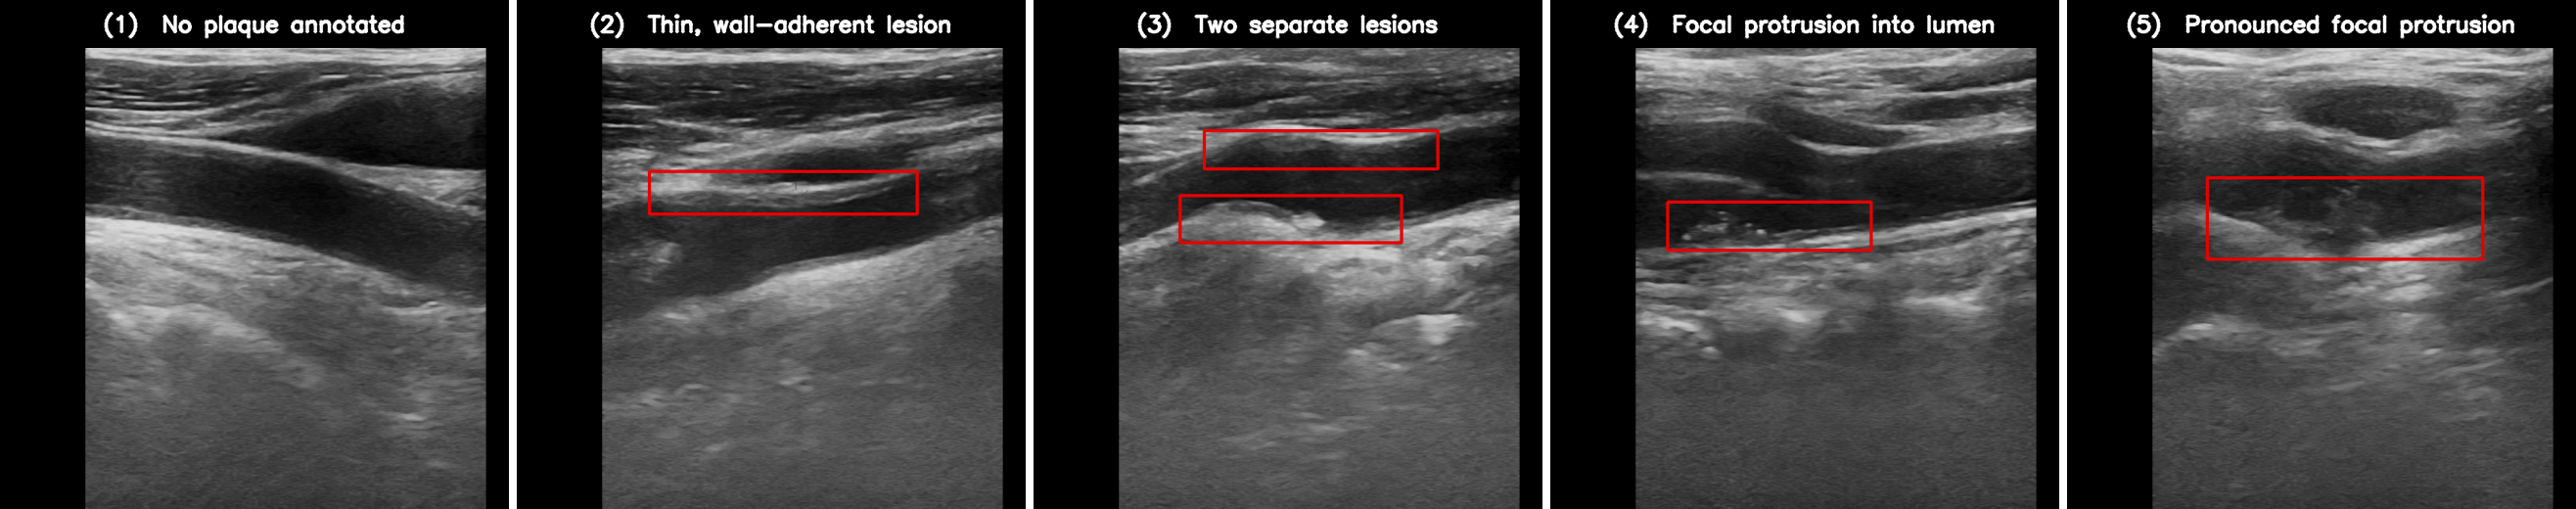
\includegraphics[width=\textwidth]{figures/plaque_progression.png}
\caption[Progression of an atherosclerotic lesion]{Lesion development and its ultrasound
appearance. Carotid artery at five stages of atherosclerotic change --
(1) unaffected vessel wall, (2) initial lipid deposition, (3) early atheroma, (4) fibroatheroma
with a lipid core beneath a fibrous cap, and (5) a complicated lesion with calcification and a
markedly narrowed lumen -- in a B-mode image from Ar-PlaqSegm1
\cite{rulloni2025arplaqsegm1} and an illustration generated with a generative image model
(OpenAI GPT-5.6 Sol, high reasoning effort). The illustration is schematic and carries no
measurement; the prompt used to produce it is archived with the code.}
\label{fig:plaque_progression}
\end{figure}

This sequence is summarised in Figure~\ref{fig:plaque_progression}. Two transitions in it matter
for what follows: the point at which wall thickening becomes a focal protrusion, which is where
the diagnostic criterion applies, and the point at which a lipid-rich core forms, which governs
how the lesion appears in ultrasound.

Clinically, the relevance of a plaque is determined less by the degree of
stenosis it causes than by its propensity to rupture \cite{naghavi2003vulnerable}.
Lesions with a large necrotic core, a thin fibrous cap and intraplaque haemorrhage
are prone to rupture and subsequent thrombus formation, whereas heavily fibrotic or
calcified lesions are comparatively stable; this morphological distinction was
established in coronary arteries \cite{virmani2000lessons} and underlies the
characterisation of carotid lesions as well \cite{libby2021}.

It matters for imaging because the same composition that governs rupture risk also
governs acoustic behaviour: lipid-rich or haemorrhagic tissue appears echolucent
(hypoechoic) in B-mode ultrasound, while fibrous and calcified tissue appears
echogenic (hyperechoic). Figure~\ref{fig:echogenicity} shows both cases. The plaques
that are hardest to delineate against surrounding tissue are therefore, in part, the same ones
that carry the greatest clinical risk. Echolucent plaques are more common in symptomatic than
in asymptomatic patients \cite{plonski2024gsm}, and plaque echogenicity predicts future
vascular events prospectively \cite{tadokoro2014echogenicity}.

The carotid arteries are of particular interest in this context. They are
superficial and therefore accessible to non-invasive ultrasound examination, and
carotid plaque burden is regarded as a marker of systemic atherosclerosis rather
than a purely local finding: subclinical disease is typically present in several
vascular territories at once \cite{fernandezfriera2015pesa}, and carotid involvement
tracks coronary calcification \cite{laclaustra2016femoral}. Carotid plaque presence has been shown to carry
predictive value for future cardiovascular events beyond that of established
risk factors, and to outperform carotid intima-media thickness in this respect. A meta-analysis
of eleven population-based studies covering 54{,}336 participants found plaque the better
predictor of future myocardial infarction, with an area under the curve of 0.64 against 0.61 for
intima-media thickness and a relative diagnostic odds ratio of 1.35 (95\,\% CI 1.10--1.82,
$p = 0.04$) \cite{inaba2012carotid}; a pooled analysis of individual participant data reached the
same conclusion for intima-media thickness as an addition to established risk scores
\cite{denruijter2012cimt}. The margin is real but modest, which is worth keeping in view: the
ten-year infarction rate after a negative finding was 4.0\,\% for plaque against 4.7\,\% for
intima-media thickness. Standardised criteria for assessing carotid
plaque by ultrasound have been set out twice: by the Mannheim consensus, an expert panel
convened at the European Stroke Conferences \cite{touboul2012mannheim}, and in the
recommendations of the American Society of Echocardiography
\cite{johri2020recommendations}.

Assessing plaque burden at the scale of a population cohort, however, is
constrained by the assessment itself. Carotid ultrasound is operator-dependent,
image quality varies with the acquisition protocol and the device used, and
manual plaque annotation requires trained readers and scales poorly: of the
177{,}757 carotid ultrasound images available in the cohort underlying this
thesis, \textcite{omarov2024deep} annotated 680. Automated, image-based
plaque detection is therefore an attractive route to deriving individual-level
plaque phenotypes for large cohorts -- provided such a model transfers reliably
to data other than that on which it was developed, which is the question this
thesis addresses.

\section{Carotid B-Mode Ultrasound}
\label{sec:ultrasound}

B-mode ultrasound forms an image from the echoes of a transmitted pulse. Sound reflects wherever
acoustic impedance changes, and the brightness assigned to a point in the image encodes the
amplitude of the echo returned from that depth \cite{bakhru2013ultrasound}. Boundaries between
tissues of differing density and stiffness therefore appear bright, and homogeneous tissue
appears as a mid-grey texture.

The carotid artery is well suited to this. It lies a few centimetres below the skin, so a
high-frequency probe can be used and resolution is correspondingly fine, and the vessel runs
close to parallel with the skin surface, so a longitudinal section shows a length of wall rather
than a single cross-section. Blood returns almost no echo and the lumen is consequently dark,
while the vessel wall produces the double-line pattern on which the intima-media thickness is
measured: a bright lumen-intima interface, a darker media, and a bright media-adventitia
interface. A plaque appears as material protruding from the wall into that dark lumen, which is
what makes it visible at all.

What it looks like depends on what it is made of. Lipid and intraplaque haemorrhage have acoustic
properties close to those of blood and return little signal, so lipid-rich lesions appear
echolucent and can be difficult to distinguish from the lumen. Fibrous tissue and calcium reflect
strongly and appear echogenic; dense calcification reflects almost the entire pulse and casts an
acoustic shadow, obscuring whatever lies behind it. Figure~\ref{fig:echogenicity} shows the two
extremes of this range in the dataset used here. Because the appearance is graded rather than
categorical, it is often quantified as the grey-scale median of the lesion after normalising the
image against reference structures, which makes values comparable between examinations
\cite{plonski2024gsm}.

Three properties of the modality bear directly on what an automated model can and cannot do with
these images. The first is speckle. The granular texture filling apparently homogeneous tissue is
not structure but interference between echoes from scatterers too small to resolve individually.
It is deterministic for a fixed geometry and changes with any shift of the probe, so it is
reproducible within an image and not between images, and a model may learn from it without the
pattern corresponding to anything anatomical.

The second is that image formation depends on choices made during the examination. Transmit
frequency, depth, focal position, overall gain and depth-dependent gain compensation all alter the
grey levels an identical structure produces, and the angle at which the probe is held alters
whether an interface reflects towards the transducer at all: a wall imaged obliquely returns a
weaker echo than the same wall imaged perpendicularly \cite{bakhru2013ultrasound}. These settings
are chosen by the operator during acquisition and cannot be recovered afterwards from the stored
image.

The third follows from the first two. A B-mode image is not a measurement of tissue in the sense
that a computed tomography number is; it is a record of how a particular vessel appeared to a
particular operator using a particular device at a particular setting. Two examinations of the
same artery may differ visibly without either being wrong. This is the source of the
operator dependence noted above, it is why plaque assessment is reported with agreement
statistics rather than as a measurement error (Section~\ref{sec:plaque-definition}), and it is
the mechanism behind the distribution shift discussed in Section~\ref{sec:domain-shift}.

\begin{figure}[H]
\centering
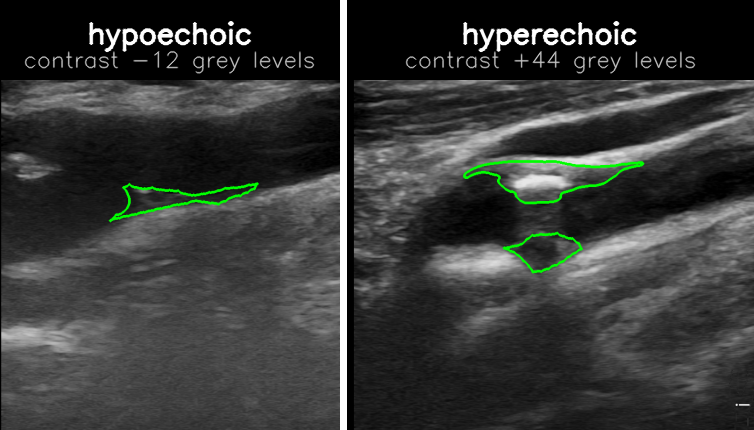
\includegraphics[width=0.82\textwidth]{figures/echogenicity.png}
\caption[Hypoechoic and hyperechoic plaque]{Two annotated images from Ar-PlaqSegm1
\cite{rulloni2025arplaqsegm1} illustrating the range of plaque echogenicity, with the annotation
outlined in green. Left: a hypoechoic lesion, 12 grey levels darker than the tissue immediately
surrounding it. Right: hyperechoic plaque, 44 grey levels brighter. The two examples have almost
the same aspect ratio, 3.9 and 4.3, so the comparison varies echogenicity while holding lesion
shape roughly constant; shape is treated separately in Figure~\ref{fig:focal-vs-diffuse}.
Contrast is the difference in mean intensity between the annotated region and a ring of 25 pixels
around it, excluding any other annotated tissue.}
\label{fig:echogenicity}
\end{figure}

\section{Plaque Definition and Annotation}
\label{sec:plaque-definition}

\begin{figure}[H]
\centering
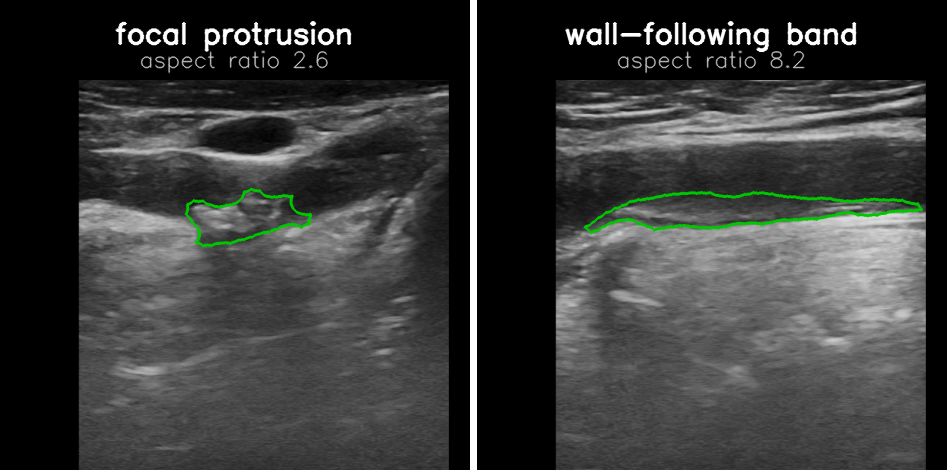
\includegraphics[width=0.82\textwidth]{figures/focal_vs_diffuse.png}
\caption[Focal and elongated annotations]{Two annotated lesions spanning the range of shapes the
plaque criterion has to accommodate, outlined in green. Left: a compact focal protrusion with an
aspect ratio of 2.6. Right: a thin band following the vessel wall over 575 pixels, aspect ratio
8.2. The criterion distinguishes focal protrusion from diffuse wall thickening, and the
boundary between them is where both the annotation and the models are least certain
(Section~\ref{subsec:results-error-analysis}).}
\label{fig:focal-vs-diffuse}
\end{figure}

The criterion this thesis works with is the one set out by the Mannheim consensus, under which a
plaque is ``a focal structure that encroaches into the arterial lumen of at least 0.5\,mm or
50\,\% of the surrounding IMT value or demonstrates a thickness $>1.5$\,mm as measured from the
media-adventitia interface to the intima-lumen interface'' \cite{touboul2012mannheim}. Two of its
three limbs are absolute and one is not, and the difference matters for everything that follows.

The absolute limbs can in principle be evaluated from the lesion alone: a thickness measurement
against a fixed threshold. The relative limb cannot. Whether a given thickening qualifies depends
on the intima-media thickness of the wall on either side of it, so the same structure is a plaque
in a vessel with a thin wall and is not one in a vessel that is uniformly thickened. The
criterion is, in this limb, a comparison rather than a property, and it is the limb that
distinguishes focal disease from diffuse wall thickening. Figure~\ref{fig:focal-vs-diffuse}
contrasts the two extremes of shape that this has to accommodate.

This has a direct consequence for an automated model. A detector or a segmentation network scores
each candidate region on its own appearance; the surrounding wall enters only in so far as it
happens to fall within the receptive field, and the model is never told that the comparison is
what defines the class. Whether it infers the comparison from examples is an empirical question
rather than a design guarantee, and Section~\ref{subsec:results-error-analysis} shows what
happens when it does not: the errors both models share are thickened wall without focal
protrusion, which is precisely the case the relative limb exists to exclude.

Applying the criterion is also not free of judgement when a human does it. Inter-sonographer
agreement for plaque detection under the Mannheim consensus has been reported at
$\kappa = 0.70$ (95\,\% CI 0.60--0.80), which is substantial but not near-perfect, and the
disagreements are systematic rather than random: lesions found in only one of two examinations
were smaller than those found in both, with a mean area of 6.82\,mm$^2$ against 11.65\,mm$^2$ and
a mean thickness of 1.45\,mm against 1.96\,mm \cite{nyman2020reproducibility}. Small plaques near
the threshold are where readers disagree with one another, and Chapter~\ref{ch:results} finds
them to be where the models fail as well.

Two implications for this thesis follow. The annotations a model is trained on are expert
judgements rather than ground truth in the physical sense, so the agreement between two readers
bounds what any model evaluated against a single reader can be expected to achieve. And because
the disagreement concentrates at the small end of the size distribution, an evaluation set with
few small lesions will overstate performance relative to one with many --- which is one reason the
composition of an external dataset, and not only its size, determines what a validation on it
means.
\section{Computational Approaches to Subclinical Atherosclerosis}
\label{sec:automated-detection}

Three kinds of data are routinely used to characterise subclinical atherosclerosis at scale:
images of the vessel, clinical and health-record variables describing the patient, and molecular
measurements from blood. Each has an established computational literature, and the three differ
in what they can resolve.

\subsection{Detection and Segmentation in Carotid Ultrasound}

The bottleneck in assessing carotid plaque across a cohort is image reading rather than image
acquisition. Of the 177{,}757 carotid ultrasound images available in the cohort underlying this
thesis, \textcite{omarov2024deep} annotated 680 -- fewer than 0.4\,\% -- because plaque annotation
requires a trained reader and per-image judgement. Automating that judgement is therefore the
prerequisite for using such images as a source of phenotypes.

Deep learning has made this tractable. Object detection frameworks such as YOLO locate
structures of interest by regressing bounding boxes with an associated confidence score
\cite{redmon2016yolo}, while segmentation architectures such as U-Net delineate them pixel by
pixel \cite{ronneberger2015unet}. In both cases transfer learning allows a model pre-trained on
natural images to be adapted to a specialised domain from a comparatively small annotated set
\cite{shin2016transfer}.
Applied to carotid ultrasound, the approach has been pursued for plaque segmentation
\cite{jain2021hybrid}, for plaque characterisation and classification
\cite{singh2024plaque}, and in a body of work surveyed by \textcite{huang2023review}.

Two features of this literature bear on the present work. The cohorts are typically clinical
rather than population-based: as \textcite{omarov2024deep} note, earlier studies have largely
addressed patients presenting with stroke or individuals with known carotid disease, which limits
how far the resulting models generalise to asymptomatic populations. And the models are
developed and evaluated within a single data source. \textcite{omarov2024deep} is the first
application at population scale, on 19{,}499 UK Biobank participants, and remains evaluated
within that cohort.

\subsection{Risk Estimation from Clinical and Health-Record Data}

An independent tradition estimates cardiovascular risk from patient characteristics rather than
from images. SCORE2 and its counterpart for older adults derive ten-year risk of a first
cardiovascular event from age, sex, smoking status, blood pressure and lipid measurements
\cite{score22021, score2op2021}. The Framingham risk profile \cite{dagostino2008framingham}
and the Pooled Cohort Equations of the American College of Cardiology and the American Heart
Association \cite{goff2014pooled} follow the same principle and are in equally wide clinical
use.

Deep learning has been applied to the same kind of data in a less constrained form. Rather than
combining a fixed set of risk factors, these models read the sequence of coded diagnoses,
medications and measurements in a health record directly \cite{rajkomar2018scalable}, and
transformer architectures developed for language have been adapted to that sequence
\cite{li2020behrt}. The most recent of them, Delphi-2M, was trained on UK Biobank records and
predicts the rates of more than a thousand diseases over the following decades
\cite{shmatko2025delphi}.

What none of these instruments do, however classical or however learnt, is observe the arterial
wall. They estimate risk from its determinants and its consequences, and consequently do not
capture subclinical disease already present in an individual whose recorded profile appears
unremarkable -- which is the gap imaging is expected to fill.

\subsection{Molecular Markers}

A third line of work seeks markers of atherosclerosis in molecules rather than in images, and it
divides by what is measured and at what cost.

At one extreme, proteomic profiling of excised plaque tissue resolves the lesion directly.
\textcite{sinha2026proteomics} analysed 112 carotid endarterectomy specimens and found that the
molecular differences between thin-capped and thick-capped plaques are spatially confined to the
necrotic core and the fibrous cap, enriched for inflammation, lipid handling and matrix
remodelling. Measurements of this kind have the highest fidelity available, because the tissue
itself is analysed, but they require the plaque to have been surgically removed. They are
therefore restricted to patients who proceed to endarterectomy, which excludes the asymptomatic
population in which subclinical atherosclerosis is defined. Notably, the same study derived a
serum protein panel predictive of plaque vulnerability, which indicates that properties of the
lesion can register in circulation.

At the other, plasma proteomic panels are now available for entire cohorts: 2{,}923 proteins have
been measured in some 53{,}000 UK Biobank participants \cite{sun2023plasma}, with comparisons
across measurement platforms established separately \cite{eldjarn2023plasma}. A blood draw
scales in a way that imaging and surgery do not, and it is non-invasive. What it observes,
however, is a systemic state, whose relation to a focal arterial lesion is not fixed by the
measurement itself but has to be established.

Between the two sits the question this thesis begins from: whether circulating proteins reflect a
lesion that has been located by imaging rather than removed by surgery. Answering it requires
both modalities in the same individuals and at a scale at which associations can be detected --
which is possible only if the lesion can be identified automatically.

\subsection{What Is Missing}

Each strand is limited in a different way, and the limitations are complementary rather than
redundant. Imaging observes the disease directly but at a cost that constrains cohort size, and
the models that automate it are rarely shown to transfer between data sources: external
validation remains the exception in medical imaging \cite{kim2019design, varoquaux2022failures}. Risk scores
scale effortlessly but infer rather than observe. Molecular panels scale and observe, but what
they observe is a systemic state whose relation to a focal arterial lesion is unestablished.

Combining them requires a phenotype that is both accurate and available at scale, and it is the
production of that phenotype -- rather than any of the three strands in isolation -- that this
thesis is concerned with.

\section{Domain Shift and External Validation}
\label{sec:domain-shift}

A model that performs well on held-out data from the cohort it was developed on may perform
substantially worse on data from elsewhere. This is not a failure of training but a
consequence of the data distribution changing between development and deployment -- commonly
termed dataset or domain shift \cite{castro2020causality}.

Ultrasound is particularly exposed to it. The image is not a direct measurement of tissue
but the result of an interaction between the tissue, the transducer, the machine's signal
processing, and the operator's choices of angle, depth, gain and focus
\cite{bakhru2013ultrasound}. Device vendor and
model, the acquisition protocol in force at a given centre, and the demographic composition
and disease prevalence of the imaged population all shift the distribution a model sees.
A model can absorb any of these as if they were features of the disease.
\begin{figure}[H]
\centering
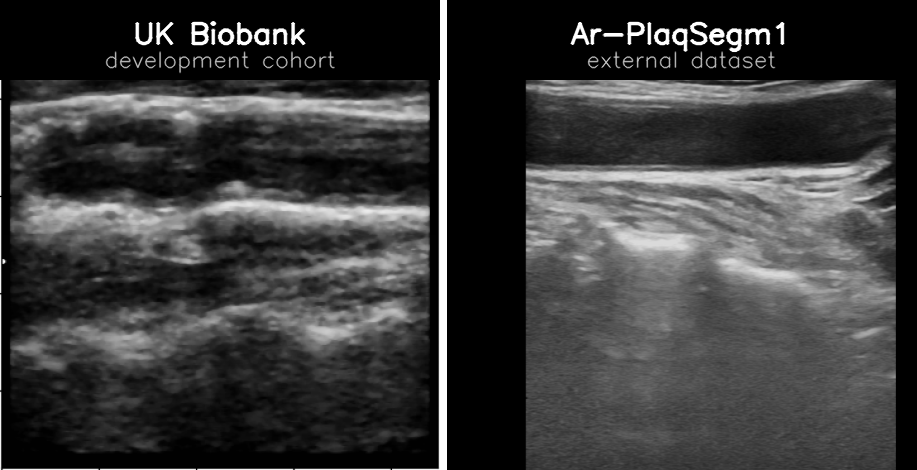
\includegraphics[width=0.86\textwidth]{figures/domain_shift.png}
\caption[Two acquisitions of the same anatomy]{The same anatomical structure recorded in the two
datasets used in this thesis, shown at a common scale. Left: a UK Biobank acquisition, the cohort
on which the base model was developed. Right: an image from Ar-PlaqSegm1
\cite{rulloni2025arplaqsegm1}, the external dataset it is evaluated on in
Chapter~\ref{ch:results}. The two differ in brightness, speckle texture and field of view
although both depict a longitudinal section of the carotid artery. Section~\ref{sec:phase2}
quantifies what such differences cost in model performance.}
\label{fig:domain-shift}
\end{figure}

Figure~\ref{fig:domain-shift} shows what this amounts to in practice for the two datasets used
here.

The effect is documented for ultrasound specifically. A model trained on one scanner loses
accuracy when applied to images from another, and recovers it only once the target device is
accounted for \cite{soylu2025migration}. A lung ultrasound classifier developed at a single
centre retained a sensitivity of 0.92 on multicentre data but fell to a specificity of 0.76,
which fine-tuning on part of that data raised to 0.82 while sensitivity stayed unchanged
\cite{wu2024generalizability} -- a pattern of preserved sensitivity and degraded specificity
that recurs in Chapter~\ref{ch:results}.

Internal validation does not detect this. Cross-validation and a held-out test set drawn
from the same cohort both estimate how a model generalises to unseen \emph{samples} of the
same distribution; neither estimates how it generalises to a different one. Reporting
standards for clinical prediction models and for artificial intelligence in medical imaging
therefore ask explicitly for validation on data external to the development cohort
\cite{collins2015tripod, mongan2020claim}. \textcite{omarov2024deep} report
five-fold cross-validation and a blind test set of 103 images, both drawn from UK Biobank;
performance outside that cohort is, by construction, not addressed by either.

In this thesis the consequence is concrete. The plaque model is not the final result: its
output is the variable that the proteomic and health-record analyses then take as their
exposure. Every participant the model labels incorrectly enters those analyses with the wrong
plaque status. Misclassification of this kind is non-differential -- the model cannot see the
protein measurements, so its errors are unrelated to the outcome -- and non-differential
misclassification biases estimated associations towards the null
\cite{copeland1977bias}. A degraded phenotype therefore weakens precisely the associations
such analyses are looking for, and does so silently, since the analysis itself gives no
indication that the exposure was measured with error. Quantifying the performance gap outside the
development cohort is therefore a prerequisite for interpreting any result derived from the
model, and reducing that gap is the subject of the second part of this thesis.

\section{Aim of This Thesis}
\label{sec:aim}

The aim of this work is to establish whether circulating proteins carry a detectable signature of
subclinical carotid atherosclerosis, and -- where that question meets its limits -- to improve the
means by which the disease is measured in the first place.

Both parts rest on the same prerequisite. Carotid plaque is not recorded as a variable in a
population cohort; it exists only implicitly, in ultrasound images that no one has read. Any
analysis relating plaque to molecular or clinical data must therefore begin by producing the
phenotype, and the quality of everything downstream is bounded by the quality of that production
step. This thesis takes that dependency as its organising principle: it derives the phenotype,
uses it, and then examines the model that produces it.

One constraint shapes the design from the outset. Carotid ultrasound and plasma proteomics were
acquired in different subsets of the cohort: the Olink panel covers 52{,}998 samples and a
plaque phenotype can be derived for 20{,}014 participants, but only 2{,}542 participants belong
to both. Any analysis relating the two directly is confined to that intersection, and the
remaining fifty thousand proteomic profiles cannot contribute, because no imaging exists for
them.

The original objective of this work addressed that constraint rather than accepting it. Health
records, unlike imaging, are available for essentially the whole cohort. If the plaque phenotype
derived from ultrasound could be predicted from health-record variables -- a proxy plaque score,
fitted on the 20{,}014 participants for whom both are available -- then that proxy could be
evaluated for every participant with proteomic data, and the association between atherosclerosis
and the plasma proteome could be tested at twenty times the sample size. The imaging arm would
supply the ground truth; the health records would supply the reach.

Three lines of work follow from this design. The first applies the detection model of
\textcite{omarov2024deep} across the UK Biobank carotid ultrasound collection and relates the
resulting plaque phenotype to the Olink proteomic panel on the intersection of the two, protein
by protein and as a multivariate predictor. The second was to construct the proxy score and
extend the analysis to the full proteomic set; it could not be carried out, as access to the
platform holding the data ended during preparation. The third, which forms the substantive
contribution of this thesis, turns to the detection model itself: how it performs on carotid
ultrasound acquired outside the cohort it was developed on, whether a model formulation matched
to the available annotations improves on it, and what limits the result. The dependency runs in
one direction throughout -- the proxy score would have been fitted against the imaging phenotype,
so its ceiling is set by the quality of that phenotype, which is what the third line of work
addresses.

The specific objectives are:

\begin{enumerate}[nosep]
  \item to reproduce the detection pipeline of \textcite{omarov2024deep} on the full set of
        UK Biobank carotid ultrasound images, and to derive individual-level plaque presence
        and plaque counts from it;
  \item to test whether the resulting plaque phenotype is associated with plasma proteomic
        profiles, both protein by protein and as a multivariate predictor;
  \item to construct a health-record-based proxy for that phenotype, so that the proteomic
        analysis is no longer restricted to the small subset of participants who have both
        imaging and proteomic measurements;
  \item to quantify the performance of that model on an external dataset of B-mode carotid
        ultrasound images, and thereby the magnitude of the distribution shift between its
        development cohort and an independent one;
  \item to fine-tune instance segmentation models on that dataset, which consume the available
        pixel-level annotations directly rather than reducing them to bounding boxes, and to
        evaluate them under a protocol that selects every operating point on validation data
        rather than on the test set; and
  \item to characterise the errors that remain, and to establish which component of the model --
        segmentation quality, instance ranking, or the image-level decision -- constrains its
        performance.
\end{enumerate}

Chapter~\ref{ch:methods} describes the data and the procedures used for each objective,
Chapter~\ref{ch:results} reports the findings, and Chapter~\ref{ch:discussion} places them
against the literature surveyed above.

\chapter{Material and Methods}
\label{ch:methods}

\section{Base Model: UK Biobank-Trained Plaque Detection Model}
\label{sec:base-model}

The starting point for this thesis is a deep learning model for automated detection of
atherosclerotic plaques in carotid ultrasound images, originally developed by
\textcite{omarov2024deep} at the Institute for Stroke and Dementia Research (LMU Munich).

\subsection{Original Training Data and Annotation}
The model was trained on carotid ultrasound images collected during the first imaging visit of
the UK Biobank cohort, following the acquisition protocol and quality-assurance procedure
described by \textcite{coffey2017protocol}. From a pool of 177{,}757 raw images across 19{,}499 participants,
38{,}732 images acquired in the longitudinal axis of the left and right distal common carotid
artery and the bifurcation were retained for analysis, and plaque annotation was performed on a
subset of these. Participants had a mean age of 64.6 years (SD 7.59) at the time of the carotid
ultrasound examination, 50.8\,\% were female, and 1{,}381 (7.1\,\%) had a baseline diagnosis of
atherosclerotic cardiovascular disease. Plaques were manually annotated by trained clinicians in
680 randomly selected images, following standard criteria \cite{touboul2012mannheim} (focal
protrusion into the arterial lumen with a thickness exceeding 50\,\% of the surrounding carotid
intima-media thickness). A plaque was present in 253 of the 680 annotated images.

\subsection{Model Architecture and Training}
\textcite{omarov2024deep} employed a YOLOv8l object detection architecture
\cite{jocher2023ultralytics}, pre-trained on a large corpus of natural images and subsequently
fine-tuned via transfer learning on the annotated carotid ultrasound subset. The annotated data
were split into training, validation, and test sets at a ratio of 0.725/0.125/0.15. To improve
generalizability, roughly half of the training images were augmented using the Albumentations
library \cite{buslaev2020albumentations} (grid distortion, brightness/contrast adjustment,
horizontal flipping, Gaussian noise, and random-sized cropping), in addition to a reduced set of
YOLOv8's built-in augmentations. Loss function weights
(distribution focal loss, box loss, and binary cross-entropy loss) were tuned via grid search,
and training used a batch size of 44 with early stopping. Five-fold cross-validation on the
development set showed consistent performance across folds, indicating limited overfitting.

\subsection{Original Model Performance}
\label{subsec:base-model-performance}
On a held-out test set of 103 images (38 containing at least one plaque), the model achieved
an image-level classification accuracy of 89.3\,\%, sensitivity of 89.5\,\%, specificity of
89.2\,\%, and a positive predictive value of 82.9\,\%, at a confidence threshold of 13\,\%
(Table~\ref{tab:base-model-performance}). The 103 test images contained 53 plaques in total. At
the object-detection level, the model reached a mean average precision at an IoU threshold of
50\,\% (mAP@50) of 68.4\,\%, with a detection precision of 70.3\,\% and a detection recall of
71.7\,\%. Applied to the full cohort, the model identified carotid plaques in 45\,\% of
participants.

The image-level figures (around 89\,\%) and the detection-level ones (around 70\,\%) answer
different questions and are not comparable with one another; Section~\ref{subsec:metrics}
sets out which of the two this thesis reports and why.

\begin{table}[H]
\centering
\caption[Original model performance]{Classification performance of the base model on the
original UK Biobank held-out test set (103 images), as reported by \textcite{omarov2024deep}.}
\label{tab:base-model-performance}
\begin{tabular}{lcccc}
\hline
& Accuracy & Sensitivity & Specificity & PPV \\
\hline
Base model (UK Biobank test set) & 89.3\,\% & 89.5\,\% & 89.2\,\% & 82.9\,\% \\
\hline
\end{tabular}
\end{table}

This baseline performance -- and, in particular, the four false negatives out of 38
plaque-positive test images -- serves as the reference point against which the external
validation and fine-tuning described in Section~\ref{sec:phase2} (Phase 2) of this thesis are
evaluated.

\section{Reproduction of the Detection Pipeline on UK Biobank}
\label{sec:reproduction}

Individual-level results of \textcite{omarov2024deep} cannot be shared directly because of UK
Biobank data-protection and access restrictions. Deriving plaque phenotypes for the analyses in
this thesis therefore required re-running the published pipeline on the UK Biobank Research
Analysis Platform rather than obtaining its outputs. Beyond reproduction, this step was also used
to derive image-level plaque counts (0--3 detections per image), which the original setup does
not provide as a standalone output but which are required downstream.

\subsection{Pipeline Adaptations}
The implementation follows the preprocessing and inference logic of \textcite{omarov2024deep} as
closely as possible. Two adaptations were made to remove manual steps that would not scale to
the full cohort. First, an alternative grey-value filtering approach was used during
preprocessing; the operation is a standard grey-level transform, and the exact step it replaced
was not recorded. Second, the selection of the relevant long-axis
(main-axis) image from each acquisition was automated. Each archive holds several frames, only
some of which show the vessel in the longitudinal plane; that view is the one the plaque
criterion is defined in, because it requires a focal protrusion to be measured against the wall
on either side of it, which a cross-sectional frame does not display.

Main-axis selection exploits a constant signature in the image data. A fixed region of the
device display is rendered identically whenever the long-axis view is active, so the sum of its
pixel values is the same in every such frame and differs in the others. Frames are therefore
matched against a reference value of 980{,}305 rather than ranked by any image property. The
value is an exact-match fingerprint of that display state and carries no meaning beyond
identifying it; it was obtained by reading it off frames known to show the long-axis view.

Matching on an exact sum is deliberate but brittle: it selects the intended frame without a
tolerance parameter, and it fails outright rather than silently returning a wrong frame if the
display state differs at all. Archives in which no frame matched were therefore recorded as
failures and excluded rather than resolved by a fallback rule. Figure~\ref{fig:ukb-pipeline} shows the sequence applied to a single acquisition.

\begin{figure}[H]
\centering
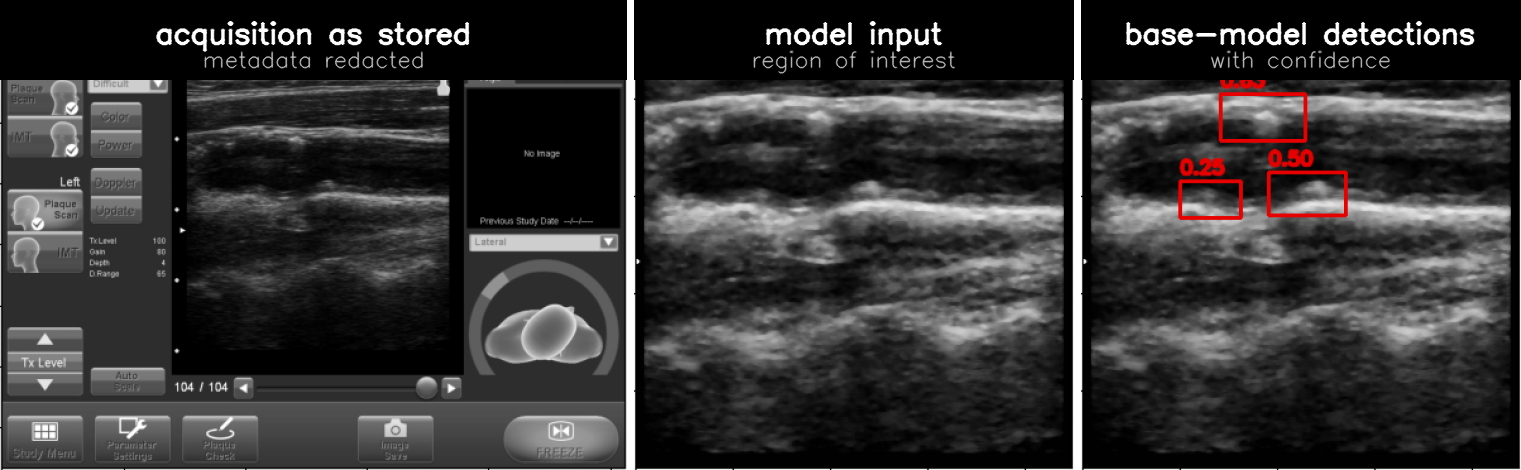
\includegraphics[width=\textwidth]{figures/ukb_pipeline.png}
\caption[The reproduced inference pipeline]{The pipeline applied to one UK Biobank acquisition.
Left: the frame as stored, comprising the full device display; the band carrying participant
identifiers and the acquisition timestamp has been redacted. Centre: the region of interest
extracted and converted to grey-scale, which is what the model receives. Right: the resulting
detections with their confidence scores, at the operating threshold of the published pipeline.}
\label{fig:ukb-pipeline}
\end{figure}

\subsection{Execution Environment}
UK Biobank data may not leave the Research Analysis Platform, so both preprocessing and inference
were executed there rather than locally. The platform provisions cloud compute instances, and
GPU-equipped instances with sufficient memory to hold the extracted image archives were used for
the inference run.
The instance was selected from the platform's mid-range GPU category, described there as
suitable for training smaller models and running machine-learning workflows. The exact
specification was not recorded at the time of the run and the platform's instance catalogue
changes over time, so a reader repeating the work should select by that category rather than by
an instance identifier.

\subsection{Scale of the Reproduction}
\label{subsec:reproduction-scale}
Inference was run over 43{,}636 archives, comprising 179{,}611 images from 20{,}014 participants
(89{,}843 left-side and 89{,}768 right-side images). For comparison, \textcite{omarov2024deep}
report a pool of 177{,}757 images across 19{,}499 participants, indicating that the reproduction
covered essentially the same image set.

Main-axis selection reduced this to 42{,}954 images from 19{,}778 participants, a reduction of
76\,\%, retaining one long-axis image per side for the large majority of participants (one left
image for 17{,}854 and two for 1{,}765 participants; one right image for 17{,}982 and two for
1{,}794). No matching frame was found in 682 archives (433 left, 249 right). The original study
retained 38{,}732 longitudinal-axis images by comparison, so the automated selection used here
keeps approximately 11\,\% more images per cohort. Per-participant plaque status was then derived
from the retained images, yielding the binary phenotype used in Phase 1A. Counts are reported in
Section~\ref{sec:results-reproduction}.

\section{Phase 1A: Proteomics Association Analysis}
\label{sec:phase1}

With individual-level plaque phenotypes available, the first analysis asked whether plasma
proteomic profiles are associated with plaque status, both at the level of individual proteins
and as a multivariate predictor.

\subsection{Proteomics Data and Analysis Cohort}
\label{subsec:phase1a-analysis}
Protein expression data were taken from the UK Biobank Olink proteomics panel
\cite{sun2023plasma}, comprising 2{,}923 proteins measured in 52{,}998 samples.
Samples and proteins were assessed for missingness prior to analysis; a descriptive overview is
given in Section~\ref{sec:results-phase1}. Merging the proteomics data with the model-derived
plaque phenotypes yielded an analysis cohort of 2{,}542 participants, of whom 1{,}066 (41.9\,\%)
were plaque-positive and 1{,}476 (58.1\,\%) plaque-negative. Age and sex were obtained from the
UK Biobank baseline assessment (fields \texttt{p21022} and \texttt{p31}).

One caveat applies to the age variable. Field \texttt{p21022} records age at recruitment, whereas
the plaque phenotype derives from the first imaging visit, which took place several years later,
and the interval between the two varies between participants. \textcite{omarov2024deep} report a
mean age of 64.6 years (SD 7.59) at the time of the ultrasound examination, against a recruitment
age range of 40--70 in the present analysis cohort. The clinical baseline reported in
Section~\ref{subsec:results-phase1a} therefore uses an age variable that is both systematically
shifted and additionally noisy relative to the outcome it is paired with.

Missing protein values were imputed with the per-protein median and all features were standardised
to zero mean and unit variance. It should be noted that imputation and scaling were fitted on the
full analysis cohort rather than within each cross-validation fold. This constitutes a mild form
of information leakage; because both operations are unsupervised and any resulting bias acts in
the direction of optimistic performance estimates, it does not weaken the null result reported
below.

\subsection{Statistical Analysis}
Three complementary approaches were applied.

At the univariate level, each protein was screened individually for association with plaque
status. Two screens were carried out. The first used a non-parametric test with
Benjamini-Hochberg correction and was summarised as a volcano plot. The second used an ANOVA
$F$-test across all 2{,}923 proteins. Age was included as an internal positive control: a screen
that detects no association at all cannot distinguish an absent signal from a failed procedure.

Access to the platform was lost before the outputs of the first screen were written out, and
they cannot be reconstructed. Section~\ref{sec:results-phase1} therefore reports the second screen in
full and the first only in outline, and no volcano plot is shown. The two screens agreed in
outcome, and the quantitative statements made in this thesis rest on the reproducible one.

At the multivariate level, five-fold stratified cross-validation (shuffled, fixed random seed) was
used to estimate the area under the receiver operating characteristic curve (ROC-AUC) for
regularised logistic regression with both L1 and L2 penalties, a random forest, and a gradient-
boosted tree ensemble (XGBoost) \cite{chen2016xgboost}. Univariate feature preselection
(ANOVA F-test, retaining the top 50, 100, 200, 300 or 500 proteins) was evaluated in combination
with these classifiers.

To separate proteomic signal from the contribution of basic demographic variables, an incremental-
value analysis compared three feature sets under the identical cross-validation scheme: age and
sex alone as a clinical baseline, proteins alone, and the combination of both.

Finally, principal component analysis was applied to the standardised protein matrix as an
exploratory check, with the first two components visualised and coloured by plaque status and by
age.

\section{Phase 1B: Electronic Health Records and Cardiovascular Risk Scores}
\label{sec:phase1b}

Phase 1A tested the biomarker hypothesis against the plaque phenotype exactly as the detection
model produces it: a single binary label per participant. Phase 1B was intended to improve that
phenotype before repeating the search, by drawing on information the imaging model does not see.

\subsection{Rationale and Study Design}
The plan was to derive an established cardiovascular risk estimate for the same cohort from the
baseline assessment and the health record, and to use it in two ways.

First, the model-derived plaque labels would be validated against it. Carotid plaque burden and
cardiovascular risk are known to be associated, so a plaque phenotype carrying genuine signal
should track the score; this constitutes a construct-validity check on the output of
\textcite{omarov2024deep} against data entirely independent of the images.

Second, the biomarker search of Phase 1A would be repeated against the risk estimate itself,
testing whether a continuous measure carrying richer clinical information yields proteomic
associations where a binary imaging-derived label did not. It should be noted that SCORE2
estimates overall cardiovascular risk and is therefore conceptually distinct from the presence
or absence of carotid plaque; the two are related but not interchangeable, and a positive
finding would have identified biomarkers of cardiovascular risk rather than of plaque
specifically.

Taken together the two analyses would also have located the null result of Phase 1A. Were the
risk estimate associated with protein expression while the plaque phenotype was not, the
limiting factor would lie in the phenotype; were neither associated, it would lie in the
proteomic data or in the size of the analysis cohort.

\subsection{Risk Score and Data Sources}
SCORE2 was selected as the risk measure \cite{score22021}. It
estimates the ten-year risk of a first fatal or non-fatal cardiovascular event in apparently
healthy individuals aged 40--69 from age, sex, smoking status, systolic blood pressure, total
cholesterol and HDL cholesterol, and is calibrated separately for four European risk regions,
with the United Kingdom falling into the low-risk region. For participants aged 70 and above,
the corresponding SCORE2-OP model would have been applied
\cite{score2op2021}.

It is worth stating precisely which data source supplies which variable, as the two are commonly
conflated. The SCORE2 predictors themselves are drawn from the UK Biobank baseline assessment --
the touchscreen questionnaire, nurse-led physical measurements and the blood biochemistry panel --
rather than from electronic health records. Health-record data are required instead for the
applicability criteria of the score. SCORE2 is derived for and intended to be applied to
individuals aged 40 to 69 without previous cardiovascular disease and without diabetes
\cite{score22021}; chronic kidney disease is not a formal exclusion, but renal function was
unavailable in the derivation cohorts, and the authors note that interpretation may require
clinical judgement in such individuals.

Ascertaining previous cardiovascular disease and diabetes would have used the UK Biobank first
occurrence fields \cite{ukbiobank_firstocc} rather than a hand-assembled code list. These fields
record, for each three-character ICD-10 code, the earliest date on which it was registered in any
of four sources -- hospital inpatient records \cite{ukbiobank_hesin}, primary care records, the
death register and self-reported conditions at an assessment visit -- together with which source
recorded it first. Relative to querying the hospital inpatient tables directly, this captures
conditions that never led to an admission, and it avoids the situation in which two studies
report the same exclusion criterion having applied different code sets to it. The relevant codes
fall in ICD-10 chapter IX for cardiovascular disease and in the diabetes mellitus block of
chapter IV.

\subsection{Electronic Health Records and Language-Model-Derived Phenotypes}
\label{subsec:phase1b-ehr}
A second, complementary direction was planned for the same phase. Rather than deriving a single
scalar risk estimate, the intention was to apply a domain-adapted large language model --
MedGemma, a family of medical vision-language models \cite{sellergren2025medgemma} -- to UK
Biobank electronic health records in order to extract clinically meaningful phenotypes and
disease trajectories. The question was whether phenotypes derived from the longitudinal health
record exhibit stronger associations with plaque status than plasma proteomics alone, and whether
trajectory information adds signal beyond a cross-sectional risk score.

That the longitudinal record carries information of this kind has since been demonstrated on the
same cohort. Delphi-2M, a generative transformer trained on UK Biobank records, predicts the
rates of more than a thousand diseases from a participant's history \cite{shmatko2025delphi}. It
differs from the design planned here in operating on coded diagnosis sequences rather than
reading the record with a language model, but it establishes the premise that design rested on,
and it would be the natural starting point were the analysis resumed.

\subsection{Current Status}
\label{subsec:phase1b-discontinuation}
Neither analysis was carried out. Access to the UK Biobank Research Analysis Platform ended while
the variables required for the risk score were being extracted, and with it access to the
baseline assessment fields, the health-record fields and the proteomic data. Both analyses are
therefore on hold; access had not been restored at the time of writing, and their resumption is
discussed in Section~\ref{sec:conclusion-outlook}.

\section{Phase 2: External Validation and Fine-Tuning}
\label{sec:phase2}

Phases 1A and 1B both take the plaque phenotype as given and ask what it is associated with.
Phase 2 returns to the ultrasound images the phenotype is produced from, and to the detection
model that produces it. It asks how the model of \textcite{omarov2024deep} performs on carotid
ultrasound acquired outside the cohort it was developed on, whether a model formulation matched
to the available annotations improves on it, and what limits the result. The evaluation uses an independent public dataset and a protocol in
which every operating point is chosen on validation data.

\subsection{External Dataset}
\label{subsec:external-dataset}
External validation used Ar-PlaqSegm1, described by its authors as the first Argentine database
of B-mode ultrasound images for atherosclerotic plaque segmentation
\cite{rulloni2025arplaqsegm1}. It provides 541 image pairs, each consisting of an 8-bit
monochrome B-mode image at $800 \times 800$ pixels and a corresponding binary plaque mask. Of
these, 340 contain one or more plaques and 201 contain none.

\subsubsection*{Acquisition and annotation}
Images were acquired at the Centro Privado Blossom DMO in C\'ordoba, Argentina, using two B-mode
ultrasound devices from different manufacturers (Esaote and Vinno). The source material comprises
26 pairs originally in DICOM format at $800 \times 600$ pixels and 515 pairs in PNG format at
$1200 \times 900$ pixels, resampled by the dataset authors to a common $800 \times 800$ grid.
Ground truth was established by two physicians experienced in manual plaque delineation, who
marked plaque boundaries on the original images; the resulting binary masks were validated by
medical specialists. The study protocol was approved by the Institutional Independent Ethics
Committee of the National University of C\'ordoba and the Rusculleda Foundation.

\subsubsection*{Case mix}
Patients were of varying age and sex and were included on the basis of mild, moderate or severe
atherosclerosis with a vascular wall thickness exceeding 1\,mm. Ar-PlaqSegm1 is therefore a
clinically enriched sample rather than a population sample, and its plaque prevalence of
62.8\,\% is correspondingly higher than the 45\,\% \textcite{omarov2024deep} report for the UK
Biobank imaging cohort. This matters for the interpretation of the external validation in
Section~\ref{subsec:results-external-validation}: the distribution shift between the two datasets
is not confined to country, centre and device but includes the composition of the imaged
population. A model developed on an asymptomatic population cohort is evaluated here on a
population in which disease is both more prevalent and, by the inclusion criterion, more advanced.

\subsubsection*{Acquisition heterogeneity}
The dataset was acquired on two devices from different manufacturers, and the images vary
correspondingly in acquisition geometry. Measuring the horizontal extent of the non-empty image
region -- the width of the insonated sector -- separates the 541 images into discrete groups
(Figure~\ref{fig:acquisition-groups}). These groups also differ in appearance: median grey-scale
intensity ranges from 53 to 97 across them, and the variance of the Laplacian, a measure of
high-frequency content, from 44 to 77.

Sector width is a proxy rather than a device label. It conflates the imaging device, the depth
and field-of-view settings chosen by the operator, the probe used, and the resampling applied by
the dataset authors in bringing $800 \times 600$ and $1200 \times 900$ source material onto a
common $800 \times 800$ grid. The dataset as distributed names the two devices but does not
identify which of them produced a given image, so the groups cannot be attributed to one cause or
the other from the record. They are therefore described here as distinguishable acquisition
geometries and nothing more.

\begin{figure}[H]
\centering
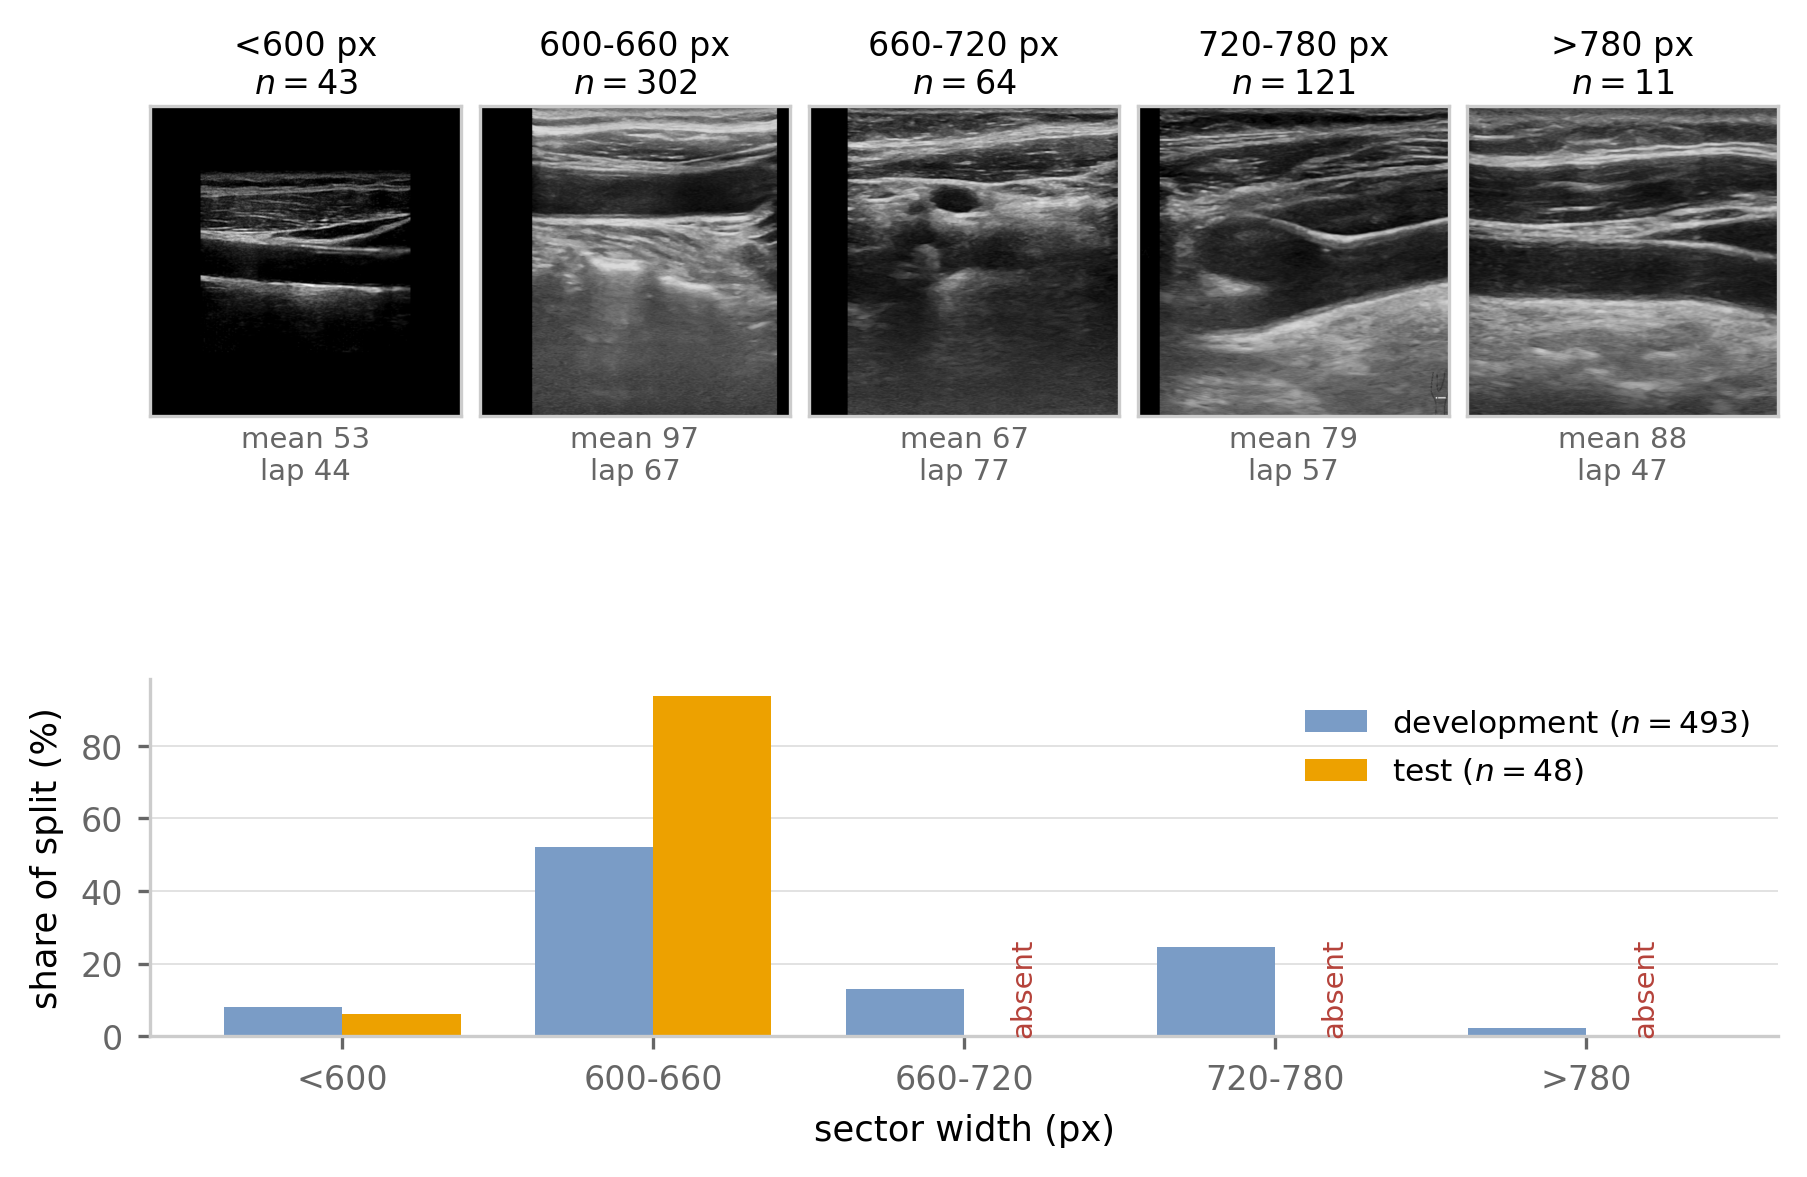
\includegraphics[width=\textwidth]{figures/acquisition_groups.png}
\caption[Acquisition heterogeneity in Ar-PlaqSegm1]{Top: a representative image from each
acquisition-geometry group, with the group's sector width, the number of images it contains, and
the median grey-scale intensity and Laplacian variance of that image. Bottom: the share of each
group in the development and test partitions. Three groups, comprising 196 of the 493 development
images, do not occur in the test partition at all.}
\label{fig:acquisition-groups}
\end{figure}

\subsubsection*{Duplicate images}
\label{subsec:duplicates}
The partition used throughout this thesis is the one distributed with the dataset; no image was
reassigned between training and test. Hashing the raw pixel data of the 541 images shows that
they comprise fewer distinct acquisitions than that number suggests: 26 groups of byte-identical
images occur, and four of these groups span both partitions of the published split, so four test
images are also present in the development partition. This overlap is a property of the dataset
as distributed rather than of any choice made here, and it applies to any evaluation that uses
the published partition without deduplicating it first. It was found by hashing the images before
training rather than inferred from the results. The consequences are quantified in
Section~\ref{sec:results-duplicates} and discussed in Section~\ref{sec:discussion-limitations},
and are deferred to there so as not to interrupt the description of the method.

\subsubsection*{Split}
The division into a development set of 493 pairs and a test set of 48 pairs is the one published
with the dataset and was adopted unchanged; it was not chosen for this thesis. The test set was
used exactly once per model, for the final evaluation reported in
Section~\ref{sec:results-phase2}. Its composition is balanced, with 24 plaque-positive and 24
plaque-negative images, while the development set contains 316 plaque-positive and 177
plaque-negative images. These counts reconcile exactly with the 340 and 201 reported for the
dataset as a whole.

The two partitions are not, however, comparable in composition. The test partition consists to
93.8\,\% of a single acquisition-geometry group, which accounts for only 52.1\,\% of the
development partition, and three of the five groups are absent from it entirely. The consequences
for the interpretation of the test results are discussed in
Section~\ref{sec:discussion-limitations}.
The dataset record does not state how many patients the 541 image pairs derive from, nor whether
the published split separates them at patient level. Image-level disjointness is verifiable and
holds apart from the duplicate groups reported above; patient-level disjointness is assumed, on
the grounds that a split constructed without it would be unusual, but it cannot be confirmed from
the material as distributed. If a patient did contribute images to both partitions, the test
figures of Chapter~\ref{ch:results} would be optimistic by an amount that cannot be estimated
here. The split is the dataset authors' own and was used unchanged, so this is a property of the
resource rather than a choice made in this work; it is recorded as a limitation in
Section~\ref{sec:discussion-limitations}.

Two properties make the dataset suitable for the purpose at hand. It originates from a different
country, imaging service and device generation, so the shift it represents is the one of
practical interest: whether a model developed on one cohort transfers to carotid ultrasound
acquired elsewhere. And its annotations are pixel-level masks rather than bounding boxes, which
permits the segmentation formulation examined in
Section~\ref{subsec:detection-to-segmentation}.

\subsection{External Validation of the Base Model}
\label{subsec:external-validation}
The base model was applied to the held-out test set to quantify the performance gap between its
development cohort and an external one. Its deployment pipeline preprocesses each image before inference: a fixed region-of-interest
crop, followed by median filtering and contrast-limited adaptive histogram equalisation. That
crop was defined for the UK Biobank image geometry and need not be appropriate for images
acquired with different devices and settings, where it may remove anatomy the model needs or
retain background it was never trained on. The model was therefore evaluated twice, once on
preprocessed and once on raw images, and the choice between the two variants was made on the
validation split rather than on the test set, for the reasons given in
Section~\ref{subsec:threshold-protocol}.

Evaluation is at the image level -- whether a plaque is detected anywhere in the image -- which is
the quantity the downstream cohort analyses consume, and which is directly comparable to the
image-level metrics reported for the base model in
Section~\ref{subsec:base-model-performance}.

\subsection{From Detection to Segmentation}
\label{subsec:detection-to-segmentation}
The annotations of the external dataset are pixel-accurate masks, whereas the base model is a
bounding-box detector. Carotid plaques are elongated structures that follow the curvature of the
vessel wall: across the 455 annotated plaque instances in the development set, the median aspect
ratio of the mask-derived bounding box is 4.6. A box drawn around such a structure consists
largely of non-plaque tissue, so the box representation discards most of what the annotation
encodes.

An instance segmentation model consumes the masks directly and, because a bounding box follows
from a predicted polygon at no additional cost, loses nothing that the detection formulation
provides. Fine-tuning was therefore carried out with segmentation models rather than detectors.
One trade-off is accepted: the warm start is a generic COCO-pretrained segmentation checkpoint
rather than the domain-specific model of \textcite{omarov2024deep}, which is detection-only and
cannot initialise a segmentation head. The domain knowledge is re-learned from the 455 annotated
polygons.

Two points follow for how the comparison in Chapter~\ref{ch:results} should be read. The first
is what is being compared. The base model is a detector trained on UK Biobank and applied to
Ar-PlaqSegm1 without adaptation; the fine-tuned models are segmentation models trained on the
Ar-PlaqSegm1 development set. They differ in two respects at once, the task they are trained on
and the data they are trained on, so a difference between them cannot be attributed to either
alone. A detection control, described in Section~\ref{subsec:detection-control}, was trained to
separate the two.

The second is what makes the comparison well defined despite the different outputs. Both
formulations produce instances carrying confidence scores, and the image-level decision --
whether a plaque is present anywhere in the image -- follows identically from both: an image is
positive if any instance exceeds the threshold. That decision is what the downstream cohort
analyses consume and is the quantity compared throughout. Mask quality, reported as the Dice
coefficient, is available only for the segmentation models, since the base model produces no
masks; no figure of that kind is compared across the two formulations.

\subsection{Dataset Construction}
\label{subsec:dataset-construction}
Each connected component of a mask was converted into one polygon instance. Components smaller
than 15 pixels were discarded as thresholding artefacts, and contours were simplified with the
Douglas-Peucker algorithm at a tolerance of 0.2\,\% of the contour arc length, which removes
near-collinear points without altering shape. Polygons with fewer than three remaining vertices
were dropped. The three representations are compared in Figure~\ref{fig:annotation-conversion}.
\begin{figure}[H]
\centering
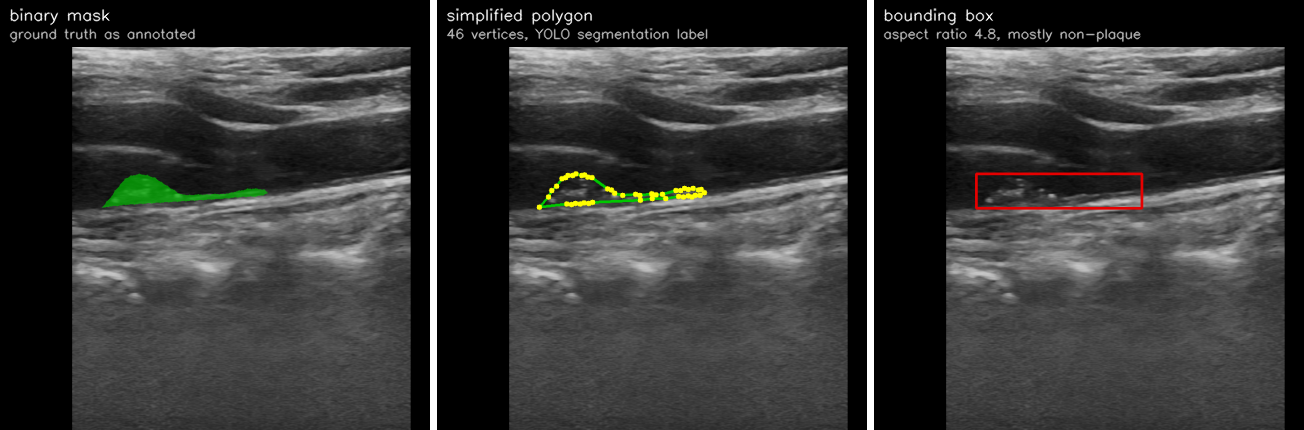
\includegraphics[width=\textwidth]{figures/annotation_conversion.png}
\caption[From mask to polygon to box]{The same annotation in three representations. Left: the
binary mask as provided with the dataset. Centre: the simplified polygon used as the
segmentation label, with its vertices marked. Right: the axis-aligned bounding box a detection
model would use instead. The box is what the detection formulation retains of the annotation.}
\label{fig:annotation-conversion}
\end{figure}
immediate rather than numerical.}
 Images annotated as plaque-free were retained with empty label files so that the
model also learns what not to detect.

The 493 development images were split into 420 training and 73 validation images, stratified by
plaque presence so that both splits retain a positive/negative mix, using a fixed random seed.
This yielded 385 polygon instances for training and 70 for validation.

\subsection{Model Training}
\label{subsec:model-training}
All models are YOLOv8 segmentation networks \cite{jocher2023ultralytics}, which extend the YOLOv8 detector
with a prototype-mask branch following the YOLACT principle \cite{bolya2019yolact}. A
\texttt{Proto} module produces 32 prototype masks at stride 4 from the highest-resolution feature
level, and each detected instance carries 32 coefficients whose linear combination, cropped to the
predicted box, forms its mask. Box regression uses distribution focal loss with 16 bins
\cite{li2020gfl}. Two model sizes were used: \texttt{yolov8m-seg} with 27{,}240{,}227
parameters and \texttt{yolov8s-seg} with 11{,}790{,}483.

Training started from COCO-pretrained checkpoints \cite{lin2014coco}, of which 411 of
417 tensors transfer; the six remaining are the class-dependent output layers, rebuilt for a
single class. Optimisation used AdamW at an initial learning rate of $10^{-3}$ decaying to
1\,\% of that value, with three warm-up epochs.

Augmentation was adapted to the modality. Vertical flipping was disabled because B-mode ultrasound
has a fixed anatomical orientation, with the probe at the top and depth increasing downwards, so a
vertical flip is physically impossible. Hue and saturation jitter were disabled because the images
are effectively greyscale, leaving brightness jitter as the only meaningful photometric variation.
Horizontal flipping (probability 0.5), rotation up to $5^\circ$, translation up to 10\,\%, scaling
up to 30\,\% and mosaic augmentation (probability 0.5) were retained.

From the second run onwards, copy-paste augmentation \cite{ghiasi2021copypaste} was enabled
at probability 0.3. This technique duplicates annotated instances into training images, so that
the model sees a greater number and variety of plaques per image than the annotations alone
provide; in the implementation used here the default mode pastes a horizontally mirrored copy of
an existing instance back into the same image. Because it operates on instance masks rather than
boxes, it is available only to the segmentation formulation and could not have been used for
detection training. It is the one segmentation-specific augmentation expected to help at this
dataset size, where 385 annotated polygons are available for training. Figure~\ref{fig:augmentation} shows one augmented batch.
\begin{figure}[H]
\centering
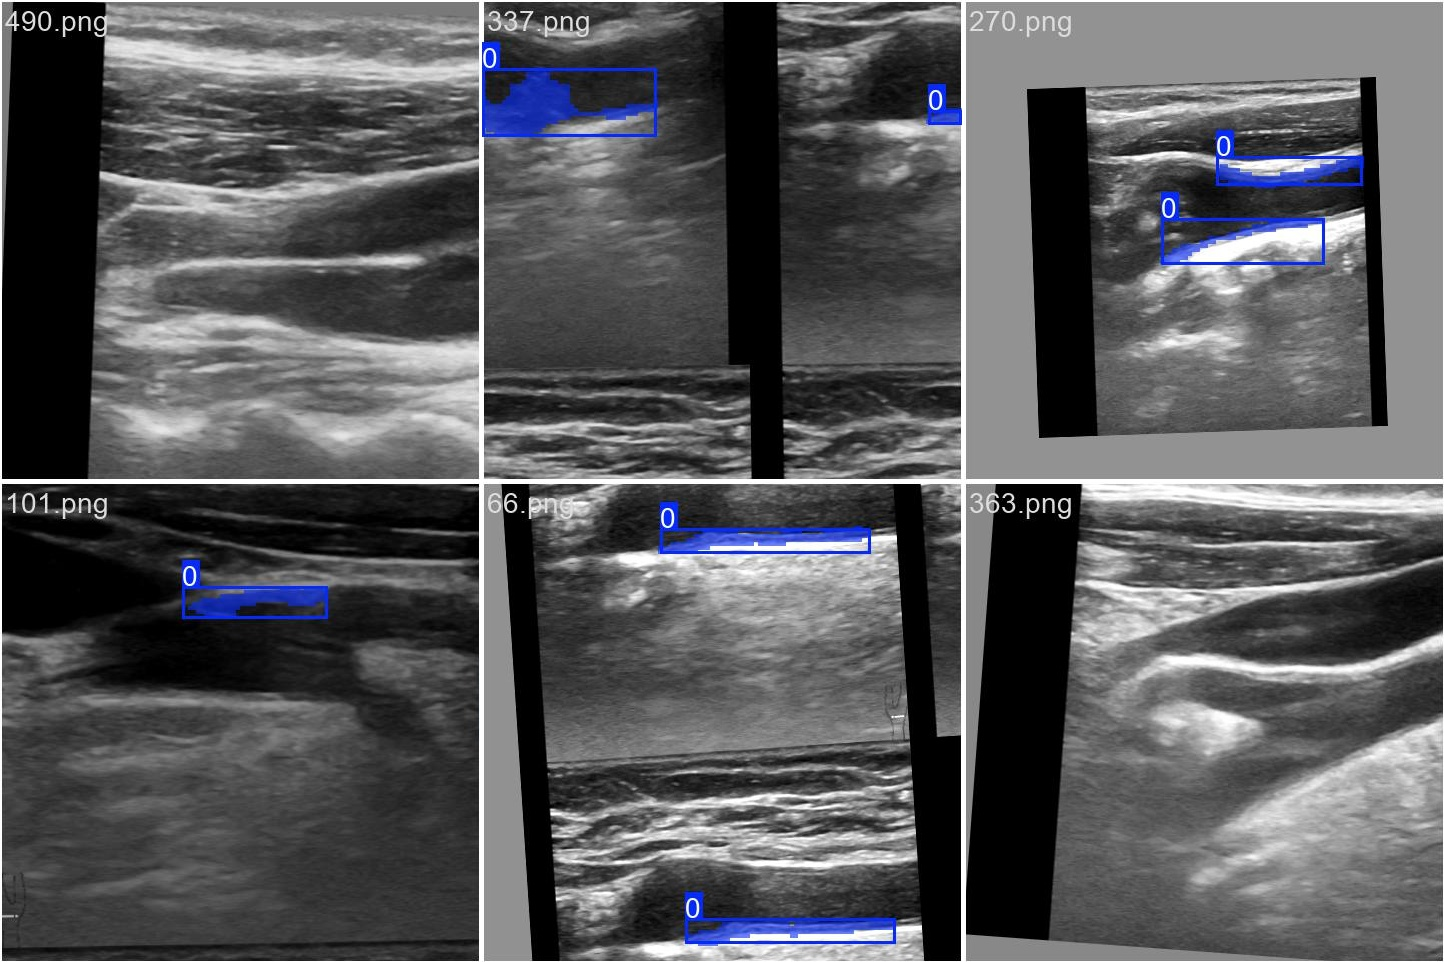
\includegraphics[width=0.85\textwidth]{figures/augmentation_batch.jpg}
\caption[An augmented training batch]{One training batch as presented to the network, written by
the training framework. Mosaic augmentation combines four images into one, and the geometric and
photometric transformations described above are applied on top; annotations are transformed with
the images.}
\label{fig:augmentation}
\end{figure}


Four models were trained (Table~\ref{tab:training-configs}). They differ in capacity, input
resolution and, from the second run onwards, in the classification loss weight. The rationale for
varying that weight is developed in Section~\ref{subsec:calibration-analysis}.

\begin{table}[H]
\centering
\caption[Training configurations]{Configurations of the four fine-tuned segmentation models. The
classification loss gain \texttt{cls} is varied systematically in the last three runs; all other
settings are held constant between them. ``Copy-paste'' denotes the instance-level augmentation
described above, which pastes mirrored copies of annotated plaques into the training images and
requires mask annotations.}
\label{tab:training-configs}
\begin{tabular}{llrrrrl}
\hline
Model & Checkpoint & Image size & Batch & Epochs & \texttt{cls} & Copy-paste \\
\hline
seg\_v1 & \texttt{yolov8m-seg} & 480 & 8  & 120 & 0.3 & no \\
seg\_v2 & \texttt{yolov8s-seg} & 640 & 16 & 226 & 0.3 & yes \\
seg\_v3 & \texttt{yolov8s-seg} & 640 & 16 & 250 & 1.0 & yes \\
seg\_v4 & \texttt{yolov8s-seg} & 640 & 16 & 250 & 0.5 & yes \\
\hline
\end{tabular}
\end{table}

Training used early stopping with a patience of 50 epochs; seg\_v2 stopped at epoch 226 of a
planned 300, while the remaining runs completed their full schedule.

All four runs were trained locally on an Apple M1 Pro with 16 GPU cores using the Metal
Performance Shaders backend. Training a single configuration to completion took approximately
5.2 hours at 250 epochs. This is distinct from the cohort-scale inference of
Section~\ref{sec:reproduction}, which ran on cloud infrastructure.

A note on the loss weighting is necessary because it becomes relevant to the results. In the
Ultralytics implementation the mask loss has no separate gain and is scaled by the box gain, so
the effective weighting of the four loss terms is 7.5 for the box loss, 7.5 for the mask loss, 1.5
for the distribution focal loss, and the value of \texttt{cls} for the classification loss. With a
single class, the classification branch is the confidence score. At the default of
\texttt{cls}~=~0.3 used in the first two runs, the term governing confidence was therefore
weighted twenty-five times lower than the terms governing geometry.

\subsection{Detection Control}
\label{subsec:detection-control}
To separate the change of formulation from the adaptation to the target domain, a bounding-box
detector was fine-tuned on the same material as the segmentation models. It used the same images,
the same split, the same schedule and the same hyperparameters as seg\_v2, with each polygon
annotation reduced to its enclosing box. It differs from seg\_v2 in its head and in the absence
of copy-paste augmentation, which operates on masks and cannot be applied to a box model. If the
segmentation formulation contributes beyond the adaptation, the detector should fall short of the
segmentation models at the image level; if it does not, the improvement over the base model is
attributable to the data rather than to the formulation. The outcome is reported in
Section~\ref{subsec:limitations-control}.

\subsection{Ensembling}
\label{subsec:ensembling}
Predictions from several models were combined by pooling. Each model is run independently at its
own training resolution, and the resulting instances are concatenated together with their
confidence scores; no averaging and no cross-model non-maximum suppression is applied. The usual
confidence threshold is then applied to the pooled set, so that an image counts as positive if any
instance from any model exceeds it, and the predicted mask is the union of the surviving
instances.

Suppression across models was deliberately avoided: for a single class it would discard precisely
those detections that only one model produced, which is the effect the pooling is intended to
exploit. The approach is motivated by the error analysis in
Section~\ref{subsec:results-error-analysis} and should be understood as a union of predictions,
not as a selection of the better one -- no information about the ground truth enters the
combination.

\subsection{Evaluation Metrics}
\label{subsec:metrics}
Three quantities are reported.

At the image level, sensitivity and specificity are computed from whether any instance exceeds the
confidence threshold, and summarised by Youden's~$J$ \cite{youden1950index}, defined as
sensitivity plus specificity minus one. This is the quantity the downstream cohort analyses
consume and the one directly comparable to the base model.

At the pixel level, agreement between the union of predicted masks and the ground-truth mask is
measured by the Dice coefficient \cite{dice1945measures}. Two aggregations are reported: the mean
over plaque-positive images, in which a missed plaque enters as zero rather than being excluded,
and a global coefficient pooling intersections and areas across the whole set, which is less
sensitive to individual small plaques.

At the instance level, mean average precision at an overlap threshold of 50\,\% (mAP@50) is
reported. A predicted instance counts as a true positive if its intersection over union with a
ground-truth instance reaches 0.5, precision and recall are evaluated across the full range of
confidence thresholds, and average precision is the area under the resulting precision-recall
curve; with a single class, the mean over classes is that value itself. The variant used here is
the mask form, in which the overlap is computed between predicted and annotated masks rather than
between boxes.

This quantity is reported for comparability with \textcite{omarov2024deep} and because the
training framework optimises against it, but it is not used to choose between models. It combines
two things this thesis separates -- whether a plaque is found at all, and how precisely it is
outlined -- and its overlap criterion is unforgiving for elongated structures, where a small
boundary error costs a disproportionate share of the intersection. Section~\ref{sec:results-phase2}
shows it diverging substantially from the image-level decision for the same models.

\subsection{Threshold Selection Protocol}
\label{subsec:threshold-protocol}
The confidence threshold is a free parameter, and choosing it on the test set would inflate the
reported performance even though no test image was trained on. All operating points reported in
this thesis are therefore selected on the validation split, by maximising Youden's~$J$ over a grid
in steps of 0.01, and then applied unchanged to the test set. For transparency, the value that
would have been obtained by optimising on the test set is reported alongside, so that the size of
the resulting optimism is visible rather than concealed.

This protocol is not fully independent: the validation split also selected the best checkpoint
during training. A strictly clean protocol would require a third split, which 493 annotated images
do not support. Choosing the threshold on validation is nonetheless substantially less circular
than choosing it on the test set.

\subsection{Error Analysis}
\label{subsec:calibration-analysis}
Two diagnostic analyses were performed beyond the headline metrics.

Confidence scores produced by modern neural networks are known to be poorly calibrated
\cite{guo2017calibration}, and two analyses were run to establish whether that is what limits
the models here.

The first isolates the contribution of confidence ranking. For each plaque-positive test image,
the best-matching predicted instance is identified irrespective of its confidence score, and the
Dice coefficient of that instance is recorded. Comparing this quantity with the Dice obtained at
the operating threshold separates two failure modes that the headline metrics conflate: a model
that does not produce a correct mask at all, and a model that produces one but ranks it below the
threshold. The median confidence carried by these best-matching instances quantifies how severely
the confidence scale is misplaced.

The second tests whether the ranking can be repaired after training. A logistic regression was
fitted on the validation split to re-score each predicted instance from features available at
inference time -- the original confidence on a logarithmic scale, mask area, aspect ratio, fill
ratio, vertical position, local echo contrast against a surrounding ring, intensity variation
within the mask, and the instance's rank and count within its image. Generalisation was estimated
by five-fold cross-validation grouped by image, since instances from the same image are strongly
correlated. The re-scored values then replaced the confidences and the standard evaluation was
repeated. Because the two scores occupy different scales, the comparison was made across matched
quantiles of each score distribution rather than at a shared absolute threshold.

Monotone recalibration methods such as Platt scaling \cite{platt1999probabilistic} or isotonic regression
\cite{zadrozny2002transforming} were not applicable: they rescale confidences while preserving
their order, and Section~\ref{subsec:results-calibration} shows the order to be the defective
property.

\chapter{Results}
\label{ch:results}

\section{Reproduction of the Detection Pipeline on UK Biobank}
\label{sec:results-reproduction}

Applying the reproduced pipeline (Section~\ref{sec:reproduction}) to the full set of UK Biobank
carotid ultrasound acquisitions yielded detections for 179{,}611 images from 20{,}014
participants. At the image level, 76.4\,\% of images contained no detection, 20.6\,\% one,
2.8\,\% two and 0.2\,\% three (Table~\ref{tab:plaque-counts}). Automated main-axis selection
retained 42{,}954 images from 19{,}778 participants; among these, 32{,}163 images carried no
detection, 9{,}318 one, 1{,}373 two and 100 three.

Aggregated to participant level, 8{,}504 of 19{,}778 participants (43.0\,\%) were classified as
plaque-positive. \textcite{omarov2024deep} report carotid plaques in 45\,\% of the cohort. Given
that main-axis selection was reimplemented independently and retains approximately 11\,\% more
images per participant than the original selection, this agreement to within two percentage
points indicates that the pipeline was reproduced faithfully at the level of the derived
phenotype, not merely at the level of the processed image count.

The prevalence is likewise consistent with the 41.9\,\% observed in the smaller proteomics
sub-cohort (Section~\ref{subsec:results-phase1a}), indicating that restriction to participants
with proteomics data did not appreciably shift the phenotype distribution.

\begin{table}[H]
\centering
\caption[Image-level plaque counts]{Distribution of detections per image before and after
automated main-axis selection.}
\label{tab:plaque-counts}
\begin{tabular}{lrrrr}
\hline
Detections per image & 0 & 1 & 2 & 3 \\
\hline
All images ($n=179{,}611$)        & 137{,}210 & 36{,}955 & 5{,}093 & 353 \\
Main-axis images ($n=42{,}954$)   & 32{,}163  & 9{,}318  & 1{,}373 & 100 \\
\hline
\end{tabular}
\end{table}

\section{Phase 1A: Proteomics Association Analysis}
\label{sec:results-phase1}

\subsection{Proteomics Dataset Overview}
The UK Biobank Olink proteomics panel comprised 2{,}923 proteins measured across 52{,}998 samples
(154{,}966{,}152 individual values in total), with an overall missingness of 10.3\,\%
(Table~\ref{tab:proteomics-missingness}). Missingness was unevenly distributed across
samples: while the median per-sample missingness was low (0.6\,\%), a distinct subset of
samples showed substantially higher missingness (up to 97.4\,\%), and 78 samples fell below
20\,\% protein coverage. Missingness across proteins followed a bimodal distribution
(Figure~\ref{fig:proteomics-missingness}), with 12 proteins falling below 80\,\% coverage. The 20
most variable proteins are shown in Figure~\ref{fig:top20-proteins}; none of them falls among
the 200 proteins with the highest missingness.
No sample or protein was excluded on the basis of missingness. The figures above therefore
describe the panel as it entered the analysis, and the missing values were handled by per-protein
median imputation rather than by exclusion (Section~\ref{subsec:phase1a-analysis}); the analysis
cohort of 2{,}542 participants results from merging the panel with the imaging-derived phenotype
and not from any quality-control filter.

\begin{table}[H]
\centering
\caption[Proteomics missingness summary]{Summary statistics of missingness in the UK Biobank
Olink proteomics panel, as it entered the association analysis.}
\label{tab:proteomics-missingness}
\begin{tabular}{lcc}
\hline
& Per sample & Per protein \\
\hline
Count & 52{,}998 & 2{,}923 \\
Mean missingness & 10.3\,\% & 10.3\,\% \\
Median missingness & 0.6\,\% & 15.4\,\% \\
Max missingness & 97.4\,\% & 99.7\,\% \\
\hline
\end{tabular}
\end{table}

\begin{figure}[H]
\centering
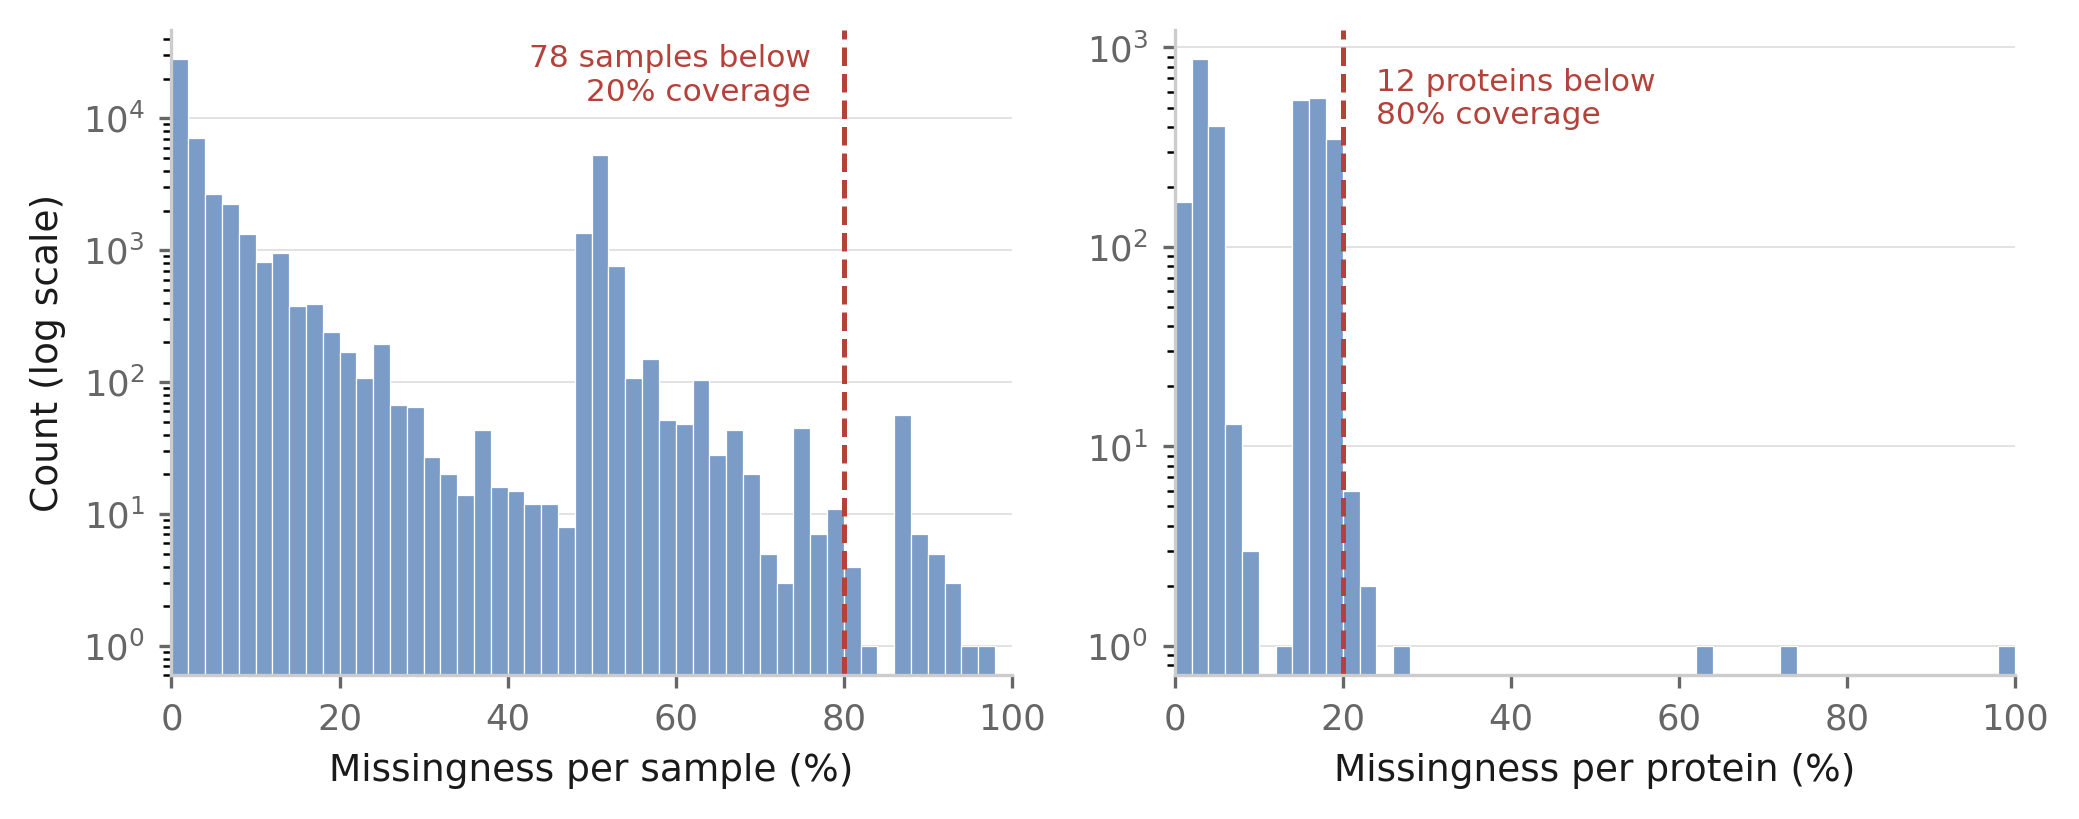
\includegraphics[width=0.95\textwidth]{figures/proteomics_missingness.png}
\caption[Missingness per sample and per protein]{Distribution of missingness per sample
(left) and per protein (right) in the UK Biobank Olink proteomics panel.}
\label{fig:proteomics-missingness}
\end{figure}


\begin{figure}[H]
\centering
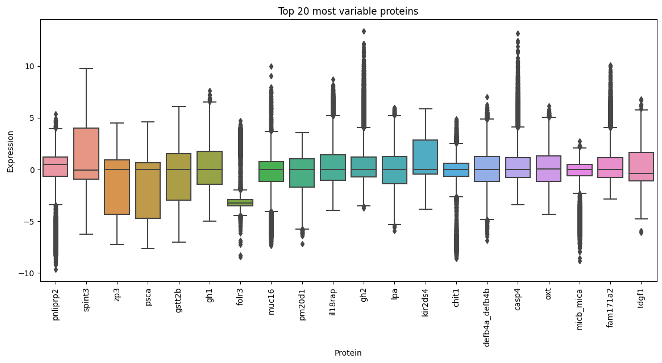
\includegraphics[width=0.85\textwidth]{figures/ukb_top20_proteins.png}
\caption[Most variable proteins]{Expression distributions of the 20 most variable proteins in the
panel. None of these falls among the 200 proteins with the highest missingness, indicating that
their variability is not an artefact of sparse measurement.}
\label{fig:top20-proteins}
\end{figure}

\subsection{Association Between Plaque Status and Proteomics}
\label{subsec:results-phase1a}

Merging the proteomics panel with the model-derived plaque phenotypes yielded 2{,}542
participants, 1{,}066 of them plaque-positive (41.9\,\%).

\paragraph{Univariate screening.}
Screening all 2{,}923 proteins individually produced 151 proteins at $p<0.05$, 37 at $p<0.01$
and 4 at $p<0.001$, with a smallest $p$-value of $5.2\times10^{-5}$ and a median $p$-value of
0.524. Under the null hypothesis, approximately 146, 29 and 3 proteins respectively would be
expected at these thresholds, so the observed counts are indistinguishable from chance. The
smallest $p$-value does not reach the Bonferroni threshold of $0.05/2923 = 1.7\times10^{-5}$,
and no protein remained significant after correction for multiple testing. Age, included in the same screen as an internal positive
control, was associated with plaque status at $p = 9.2 \times 10^{-6}$ and therefore clears the
same Bonferroni threshold that no protein reaches. The screen detects an association where one
exists; it finds none among the proteins. The strongest correlation of any single
feature with plaque status was $r = 0.088$, and that feature was age rather than a protein.

\paragraph{Multivariate classification.}
No classifier extracted usable signal from the proteomic profile
(Table~\ref{tab:phase1a-auc}). The best-performing proteomics model, gradient boosting restricted
to the 100 most informative proteins, reached a cross-validated ROC-AUC of
$0.541 \pm 0.017$; regularised logistic regression on the full panel remained at
$0.513 \pm 0.009$. All values lie close to the 0.5 expected from random classification.

\begin{table}[H]
\centering
\caption[Phase 1A classification performance]{Five-fold cross-validated ROC-AUC for predicting
model-derived plaque status from plasma proteomics ($n=2{,}542$; 2{,}923 proteins). Values are
mean $\pm$ standard deviation across folds.}
\label{tab:phase1a-auc}
\begin{tabular}{lc}
\hline
Model & ROC-AUC \\
\hline
Logistic regression (L1) & $0.508 \pm 0.011$ \\
Logistic regression (L2) & $0.513 \pm 0.009$ \\
Random forest & $0.517 \pm 0.017$ \\
XGBoost & $0.539 \pm 0.016$ \\
XGBoost, top-100 proteins & $0.541 \pm 0.017$ \\
\hline
Age and sex only & $0.551 \pm 0.028$ \\
\hline
\end{tabular}
\end{table}

\paragraph{Incremental value over demographics.}
A clinical baseline using age and sex alone reached $0.551 \pm 0.028$ and thus outperformed every
proteomics-based model. Adding proteins to this baseline did not improve discrimination but
slightly reduced it, to $0.520 \pm 0.013$ for the combination against $0.523 \pm 0.014$ for
proteins alone -- consistent with two informative variables being diluted among a hundred
uninformative ones under regularisation, rather than with any contribution from the proteome.

\paragraph{Exploratory visualisation.}
Principal component analysis of the standardised protein matrix reproduced the same picture
(Figure~\ref{fig:pca-proteomics}). The first two components capture 15.1\,\% and 4.8\,\% of the
variance. Colouring the identical embedding by age reveals a visible gradient, whereas colouring
it by plaque status shows complete overlap of the two groups. The proteomic data therefore carry
structure that these components resolve; plaque status is not part of it. As the first two
components account for only about 20\,\% of the total variance, this observation supports rather
than establishes the absence of signal.

\begin{figure}[H]
\centering
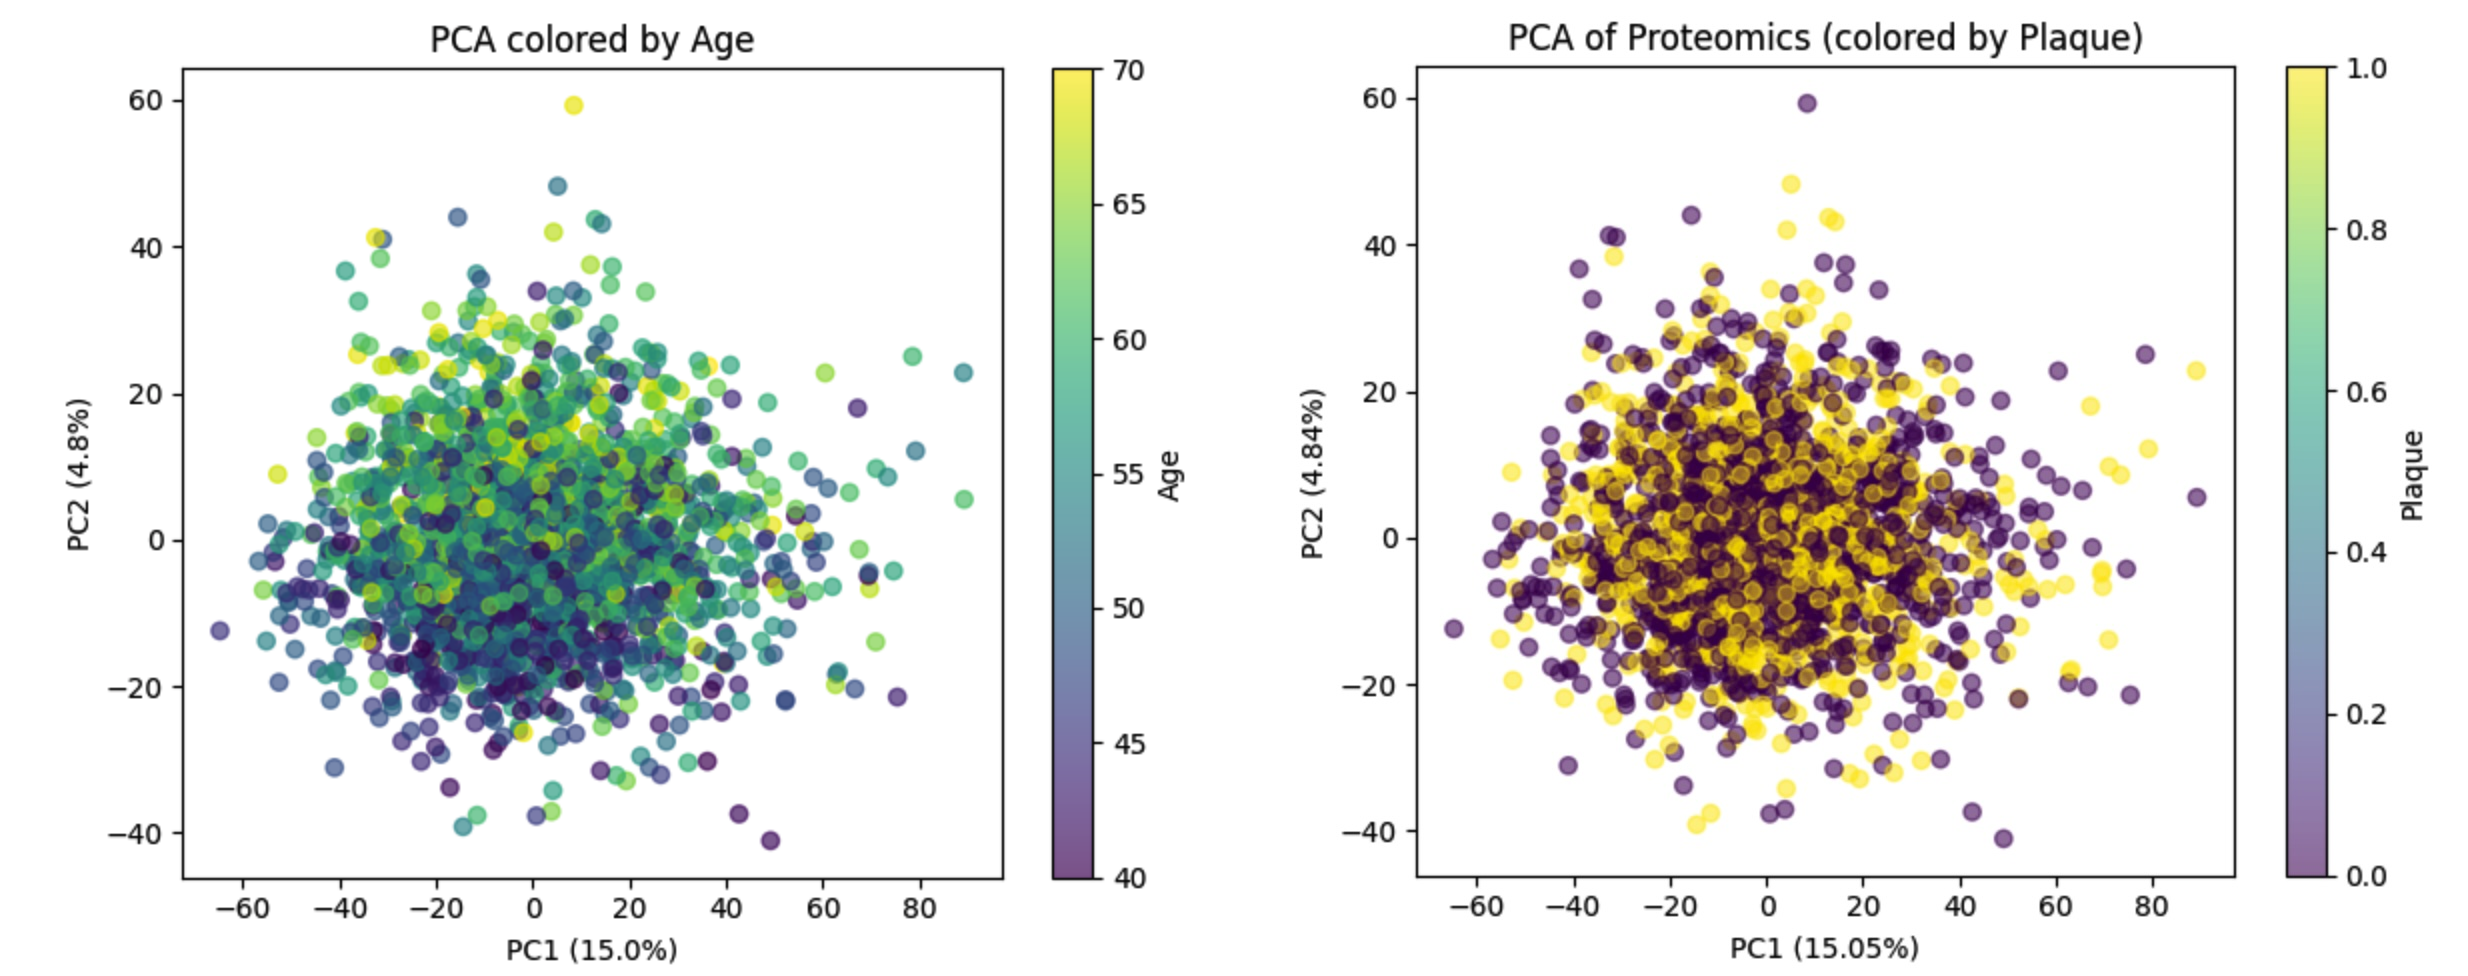
\includegraphics[width=\textwidth]{figures/pca_proteomics.png}
\caption[PCA of the proteomics panel]{Principal component analysis of the standardised protein
matrix ($n=2{,}542$). Left: coloured by age. Right: coloured by model-derived plaque status. The
same embedding separates participants by age but not by plaque status.}
\label{fig:pca-proteomics}
\end{figure}

\section{Phase 2: External Validation and Fine-Tuning}
\label{sec:results-phase2}

All results in this section use the threshold protocol of
Section~\ref{subsec:threshold-protocol}: the operating point is selected on the validation split
and applied unchanged to the 48 held-out test images.

\subsection{External Validation of the Base Model}
\label{subsec:results-external-validation}

Of the two preprocessing variants, the raw images outperformed the region-of-interest crop with
contrast equalisation on the validation split ($J = 0.493$ against $J = 0.323$), and the raw
variant was carried forward. This is consistent with the region of interest having been defined
for the UK Biobank image geometry: applied to the external images it truncates part of the
annotated plaque in 9 of the 24 plaque-positive test images, retaining as little as 64\,\% of the
annotated area in the most severe case.

On the external test set the base model reached a sensitivity of 83.3\,\% and a specificity of
62.5\,\% ($J = 0.458$). Against the 89.5\,\% and 89.2\,\% reported on its own held-out UK Biobank
test set (Section~\ref{subsec:base-model-performance}), sensitivity therefore declines by
6.2 percentage points while specificity declines by 26.7. The model continues to find plaques
that are present, but raises substantially more false alarms on plaque-free images from a source
it was not developed on.

\subsection{Performance of the Fine-Tuned Models}
\label{subsec:results-finetuned}

\begin{figure}[H]
\centering
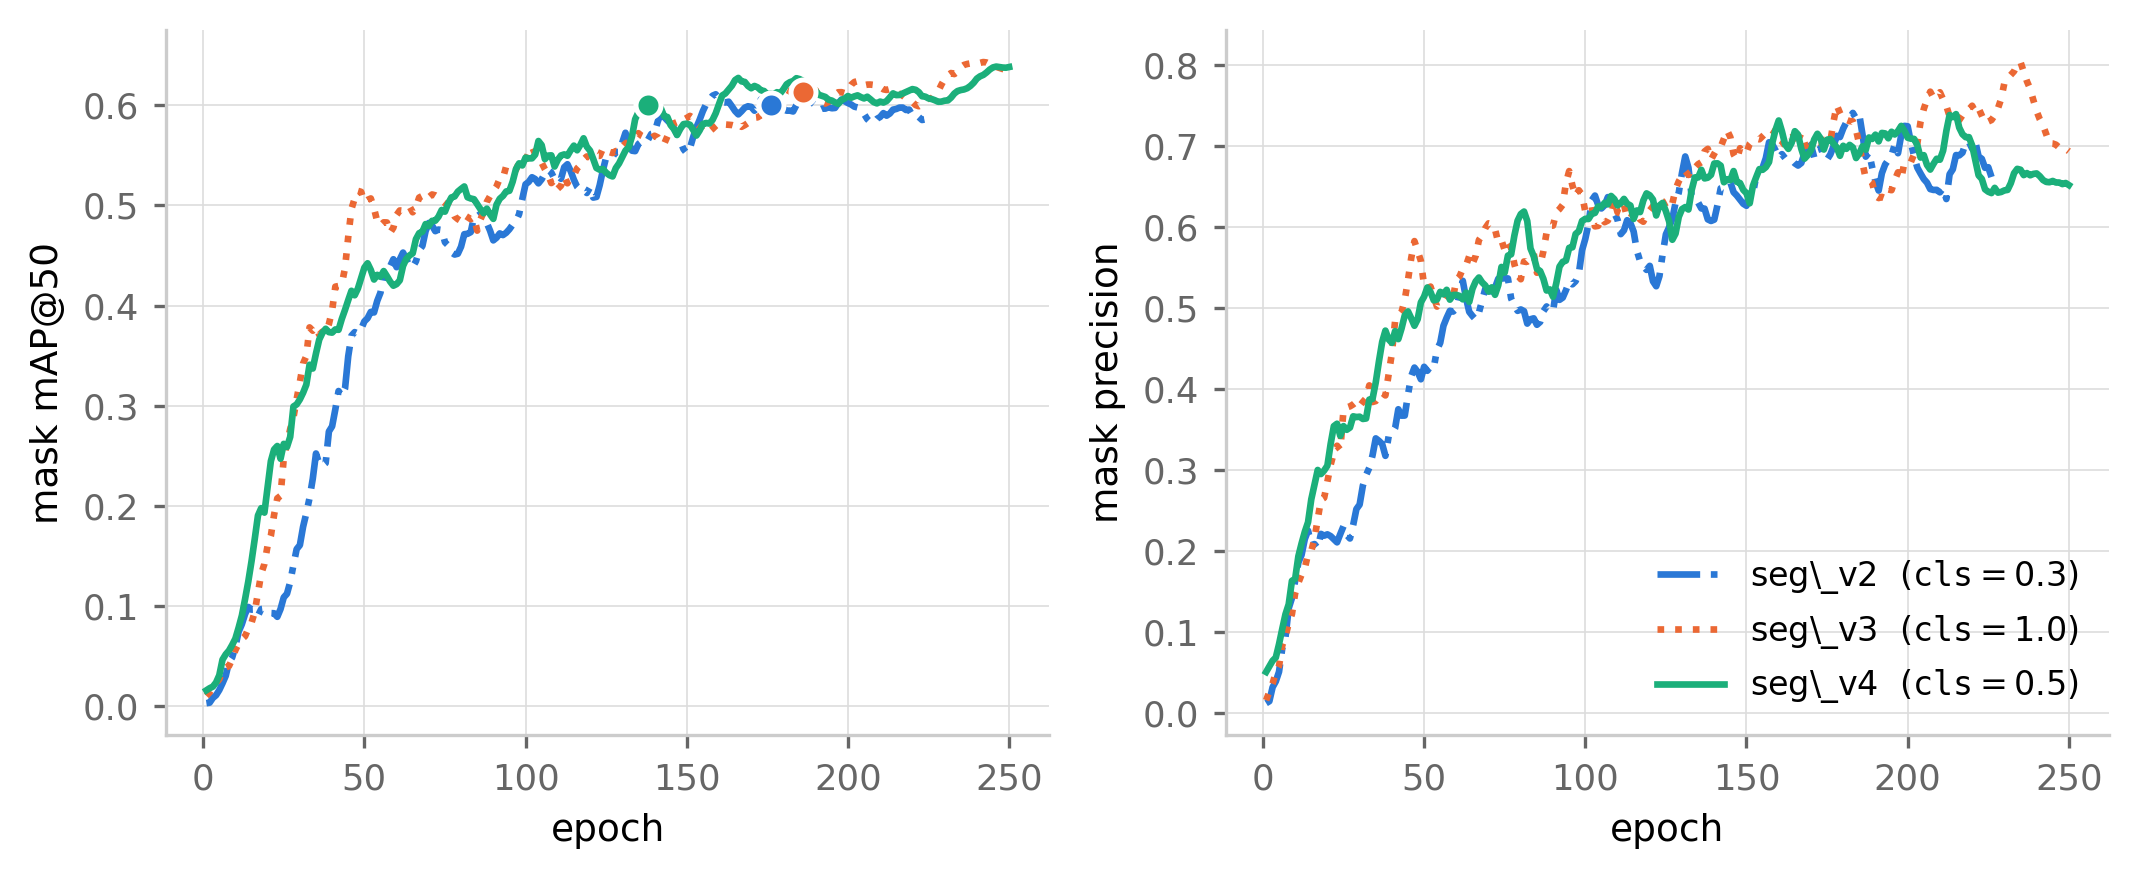
\includegraphics[width=\textwidth]{figures/cls_series.png}
\caption[Effect of the classification loss weight]{Validation mask mAP@50 (left) and mask
precision (right) over training, for the three models that differ only in the classification loss
weight. Curves are smoothed with a nine-epoch centred moving average. The marker on each curve in
the left panel gives the epoch at which that run's best checkpoint was saved, taken from the
unsmoothed values: epoch 138 for seg\_v4, 176 for seg\_v2 and 186 for seg\_v3. The higher weight
accelerates convergence and raises precision without lifting the final mAP.}
\label{fig:cls-series}
\end{figure}

On the validation split the four fine-tuned models reach a best mask mAP@50 of between 0.623 and
0.673, with seg\_v4 the strongest (Table~\ref{tab:seg-val}). On the held-out test set this
ordering does not survive: seg\_v1, seg\_v2 and seg\_v3 all reach $J = 0.625$ and differ only in
how they distribute their errors between sensitivity and specificity, while seg\_v4 -- the best
model on validation -- performs worst ($J = 0.583$).

\begin{table}[H]
\centering
\caption[Validation performance of the fine-tuned models]{Best mask mAP@50 on the validation
split, with the mask precision at the same epoch.}
\label{tab:seg-val}
\begin{tabular}{lrrr}
\hline
Model & mAP@50 (mask) & Epoch & Precision (mask) \\
\hline
seg\_v1 & 0.623 & 107 & 0.665 \\
seg\_v2 & 0.655 & 176 & 0.693 \\
seg\_v3 & 0.648 & 186 & 0.698 \\
seg\_v4 & 0.673 & 138 & 0.766 \\
\hline
\end{tabular}
\end{table}

That three models tie exactly on the test set is a consequence of its size.
Figure~\ref{fig:cls-series} shows how the classification loss weight shapes training.
 With 24
plaque-positive and 24 plaque-negative images, one image corresponds to 4.2 percentage points of
sensitivity or specificity, so differences smaller than roughly one image in each direction are
not measurable. This limitation applies to every comparison between fine-tuned variants below; it
does not apply to the comparison against the base model, where the margin is larger.

\subsection{Ensembling}
\label{subsec:results-ensembling}

Pooling the predictions of several models improves on every individual model
(Table~\ref{tab:phase2-main}, Figure~\ref{fig:roc-testset}). The combination of seg\_v1 and seg\_v2 reaches a sensitivity of
91.7\,\% at a specificity of 75.0\,\% ($J = 0.667$) with a mean Dice of 0.655. The gain is
confined to sensitivity: relative to seg\_v1 the pooled model detects one additional plaque at
unchanged specificity, while relative to seg\_v2 it detects two more at the cost of one
additional false positive. This asymmetry is structural and is examined in
Section~\ref{subsec:results-error-analysis}. Adding further models does not
help: seg\_v1\,+\,seg\_v2\,+\,seg\_v4 attains the same $J$ with higher sensitivity and lower
specificity, and the four-model combination is worse than the two-model one.

\begin{table}[H]
\centering
\caption[Phase 2 performance on the held-out test set]{Image-level performance on the 48 held-out
test images (24 plaque-positive). The threshold $t^*$ is selected on the validation split. The
final column gives the value of $J$ that would have been obtained by optimising the threshold on
the test set itself, as a measure of the optimism avoided.}
\label{tab:phase2-main}
\begin{tabular}{lrrrrrr}
\hline
Model & $t^*$ & Sens. & Spec. & $J$ & Dice & $J$ (test-optimised) \\
\hline
Base model (Omarov et al.) & 0.02 & 0.833 & 0.625 & 0.458 & -- & 0.500 \\
\hline
seg\_v1 & 0.19 & 0.875 & 0.750 & 0.625 & 0.594 & 0.708 \\
seg\_v2 & 0.18 & 0.833 & 0.792 & 0.625 & 0.576 & 0.750 \\
seg\_v3 & 0.03 & 0.792 & 0.833 & 0.625 & 0.554 & 0.750 \\
seg\_v4 & 0.22 & 0.708 & 0.875 & 0.583 & 0.502 & 0.708 \\
\hline
seg\_v1 + seg\_v2 & 0.25 & 0.917 & 0.750 & \textbf{0.667} & \textbf{0.655} & 0.792 \\
seg\_v1 + seg\_v4 & 0.25 & 0.917 & 0.708 & 0.625 & 0.619 & 0.667 \\
seg\_v2 + seg\_v4 & 0.25 & 0.833 & 0.833 & 0.667 & 0.547 & 0.708 \\
seg\_v1 + seg\_v2 + seg\_v4 & 0.25 & 0.958 & 0.708 & 0.667 & 0.655 & 0.792 \\
all four & 0.25 & 0.958 & 0.667 & 0.625 & 0.648 & 0.792 \\
\hline
\end{tabular}
\end{table}

Relative to the base model, the best configuration improves Youden's~$J$ from 0.458 to 0.667,
raising sensitivity from 83.3\,\% to 91.7\,\% and specificity from 62.5\,\% to 75.0\,\%. Roughly
half of the specificity lost to the change of data source is thereby recovered.

How much of this improvement is attributable to the segmentation formulation rather than to
adaptation to the target domain is examined by a control experiment reported in
Section~\ref{subsec:limitations-control}: a detector trained on the same data reaches the same
image-level performance as the segmentation models.

\begin{figure}[H]
\centering
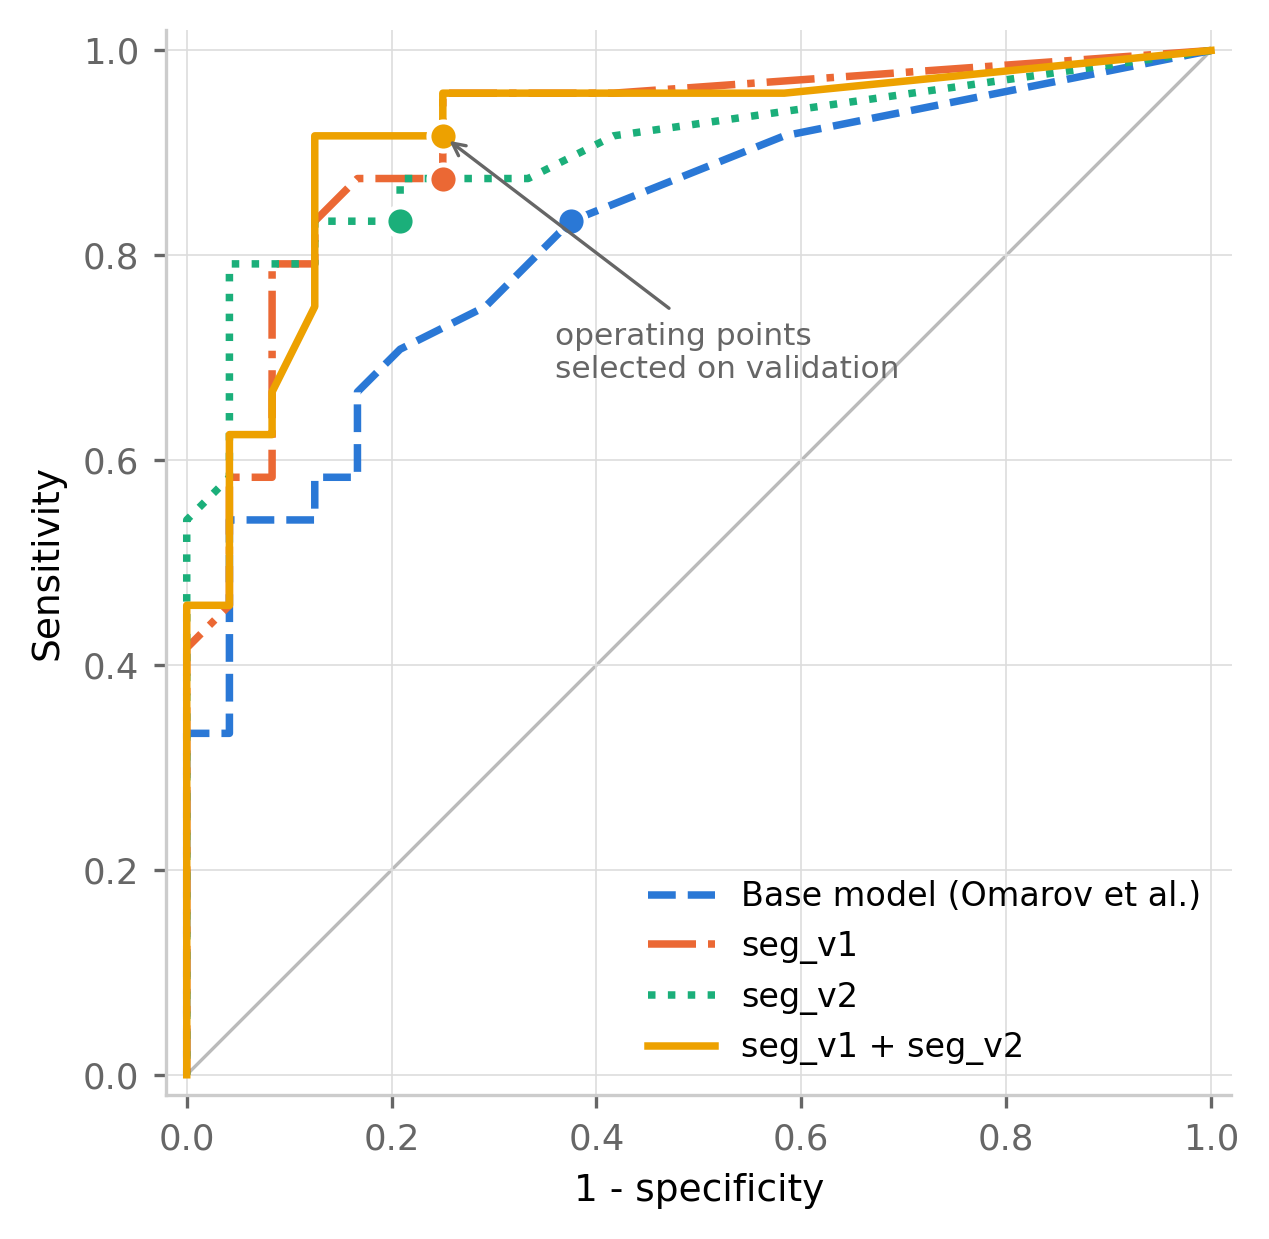
\includegraphics[width=0.62\textwidth]{figures/roc_testset.png}
\caption[Operating characteristics on the held-out test set]{Image-level operating
characteristics on the 48 held-out test images, obtained by sweeping the confidence threshold.
Markers give the operating point selected on the validation split. The base model lies below all
fine-tuned variants; pooling seg\_v1 and seg\_v2 dominates either model alone over most of the
range.}
\label{fig:roc-testset}
\end{figure}

The final column quantifies what the threshold protocol costs in reported performance. Optimising
the threshold on the test set would have raised the headline figure for seg\_v1\,+\,seg\_v2 from
0.667 to 0.792. The difference of 0.125 is of the same order as the entire improvement over the
base model, which is why the protocol matters.

\subsection{Error Analysis}
\label{subsec:results-error-analysis}

On plaque-positive images the errors of seg\_v1 and seg\_v2 are largely complementary
(Figure~\ref{fig:model-agreement}). Of the 24 plaque-positive test images, 19 are detected by
both models, two by seg\_v1 only, one by seg\_v2 only, and two by neither. Pooling therefore
recovers three images that no single model would have contributed, which is the mechanism behind
the sensitivity gain reported above.

On plaque-free images the picture is the opposite. Of the six false positives, five are shared by
both models and only one is unique. Because pooling takes the union of detections, shared false
positives cannot be removed by it, and the specificity of the pooled model is bounded by that of
its weaker constituent. This is why the improvement is confined to sensitivity, and it sets a
ceiling that no combination of these models can pass.

\begin{figure}[H]
\centering
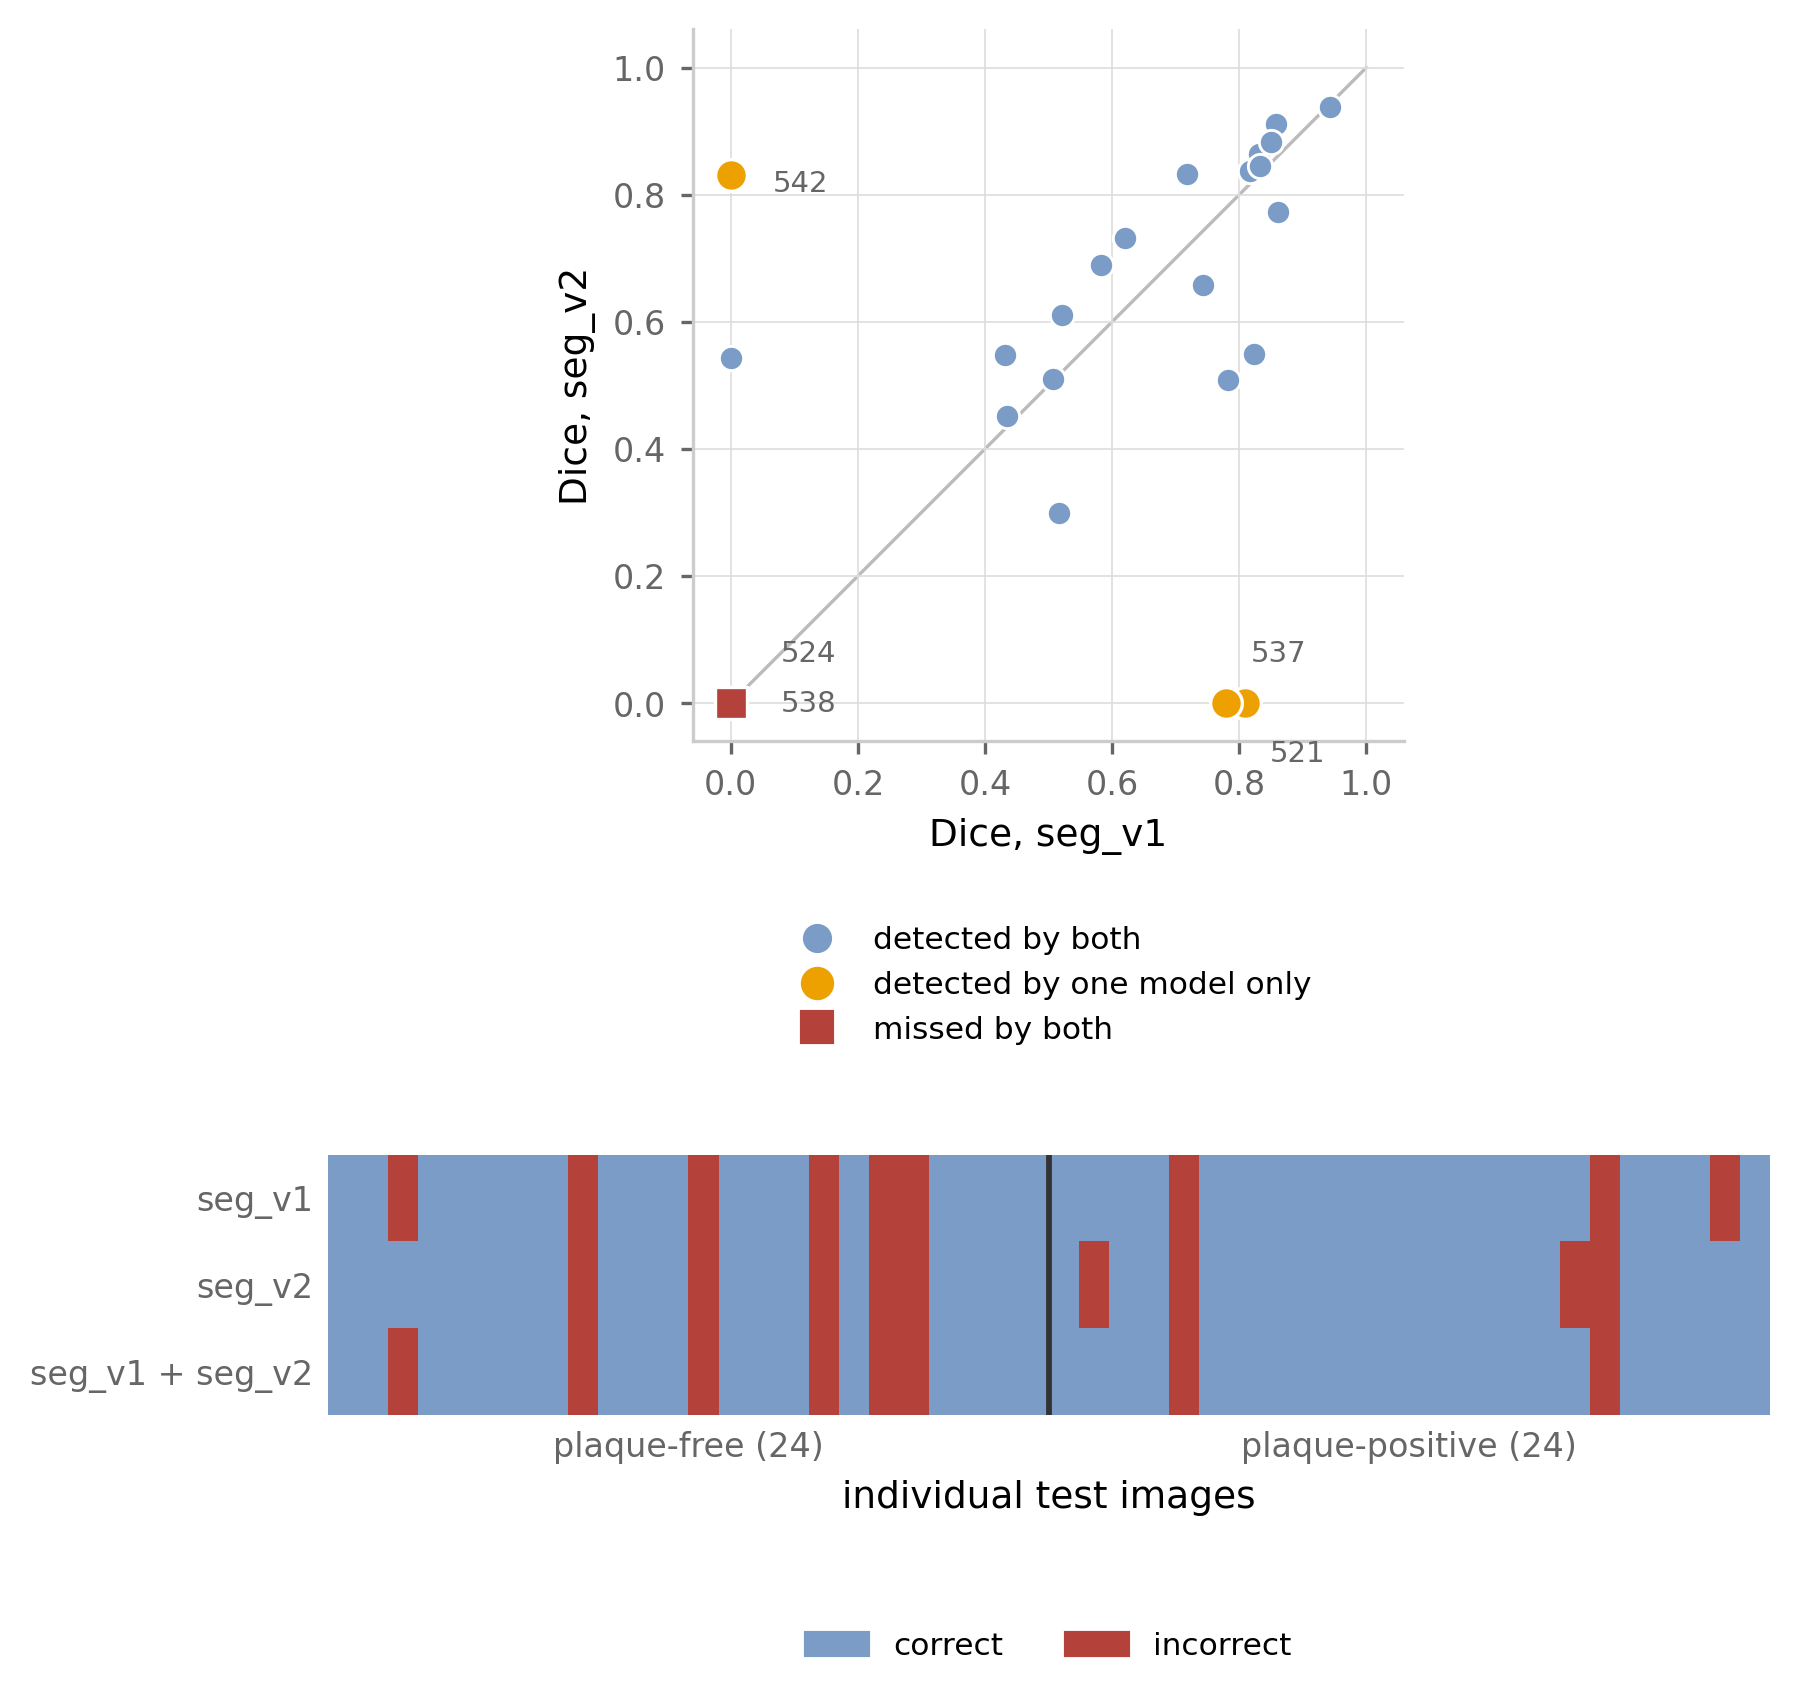
\includegraphics[width=0.72\textwidth]{figures/model_agreement.png}
\caption[Agreement between the two models]{Top: Dice coefficient of seg\_v1 against seg\_v2 for
the 24 plaque-positive test images. Bottom: per-image correctness of both models and of their
union across all 48 test images, at the operating points selected on validation. Complementarity
is present among the plaque-positive images but almost absent among the plaque-free ones.}
\label{fig:model-agreement}
\end{figure}

\subsubsection*{What the models mistake for plaque}

The shared false positives follow a single pattern (Figure~\ref{fig:false-positives}). In all six
plaque-free images that are flagged, the predicted contours follow the vessel wall over an
extended stretch rather than enclosing a focal protrusion into the lumen. Quantitatively, the
false-positive predictions are systematically thinner and smaller than true plaque annotations:
their median thickness, taken as mask area divided by bounding-box width, is 20.7 pixels against
29.9 for the annotated plaques, and their median area is 5{,}141 pixels against 9{,}705.

This is consistent with the models having learned local appearance -- a bright, elongated
structure along the wall -- rather than the diagnostic criterion itself. A plaque is defined as a
focal protrusion exceeding 50\,\% of the \emph{surrounding} intima-media thickness
(Section~\ref{subsec:external-dataset}). That criterion is relative: it requires comparing a
candidate region with the adjacent wall. A segmentation model that classifies each region on its
own appearance has no access to that comparison, and thickened but non-focal wall is precisely
the case in which the distinction matters.

\begin{figure}[H]
\centering
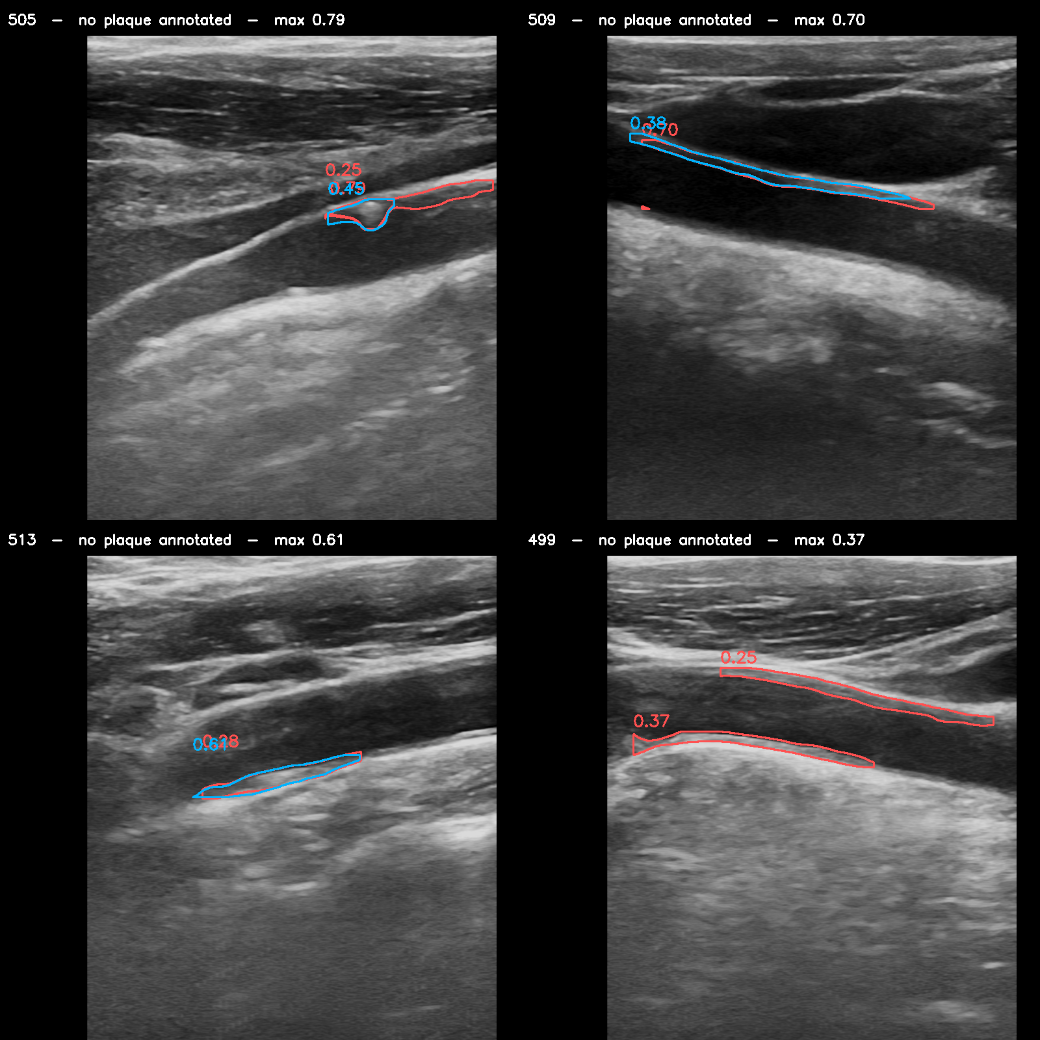
\includegraphics[width=0.78\textwidth]{figures/false_positives.png}
\caption[False positives]{Four of the six plaque-free test images that both models flag, with the
two highest-scoring contours of each model. Predictions follow the vessel wall over an extended
stretch rather than enclosing a focal protrusion.}
\label{fig:false-positives}
\end{figure}

Three candidate explanations for the residual failures were tested against the development set
and none survived. Geometry does not explain them: the mask that both models miss most severely
is at the 96th percentile of annotated area and the 90th percentile of aspect ratio, with 20
comparable instances present in the training data. Visibility does not explain them: the same
mask has a higher contrast against its surroundings than 86\,\% of training annotations. Nor does
echogenicity: the training data are evenly divided between hyperechoic and hypoechoic annotations
(157 against 159), and the difference in mean Dice between hypoechoic and hyperechoic test images
(0.580 against 0.676, on 8 and 16 images respectively) is within the noise of the sample.

\subsection{Confidence Calibration}
\label{subsec:results-calibration}

\begin{figure}[H]
\centering
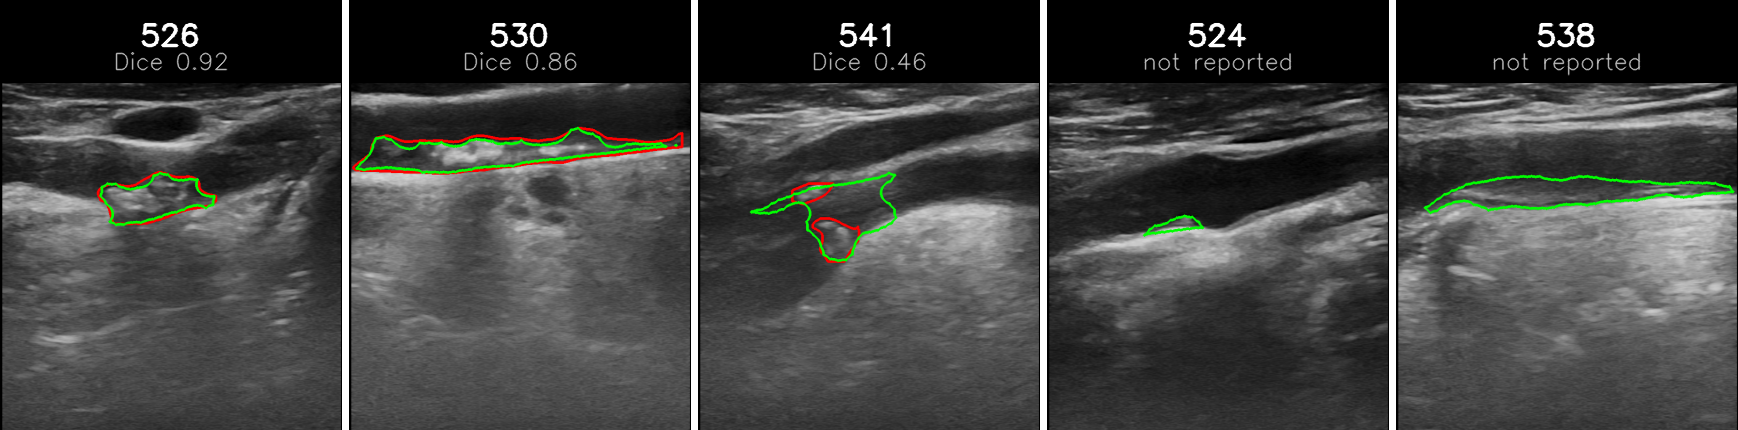
\includegraphics[width=\textwidth]{figures/qualitative_examples.png}
\caption[Qualitative examples]{Five plaque-positive test images with the annotation in green and
the pooled prediction in red, at the operating point selected on validation. The first two are
segmented accurately. The third is the only image for which no predicted instance matches the
annotation well. In the last two the models produce an accurate mask but score it far below the
threshold, so nothing is reported.}
\label{fig:qualitative}
\end{figure}

The explanation lies in the confidence scores rather than in the masks. Taking, for each
plaque-positive test image, the best-matching predicted instance irrespective of its confidence
raises the mean Dice of the seg\_v1\,+\,seg\_v2 ensemble from 0.655 to 0.794 and leaves no image
without a correct mask (Figure~\ref{fig:dice-oracle}). Both apparent failures disappear: the most severe of them is outlined at
a Dice of 0.818 by seg\_v1 and 0.789 by seg\_v2, at confidence scores of 0.0019 and 0.0010
respectively, against an operating threshold of 0.25.

The models therefore segment these plaques correctly and score them as though they were not
there. Figure~\ref{fig:qualitative} shows both behaviours alongside two successful cases. \begin{figure}[H]
\centering
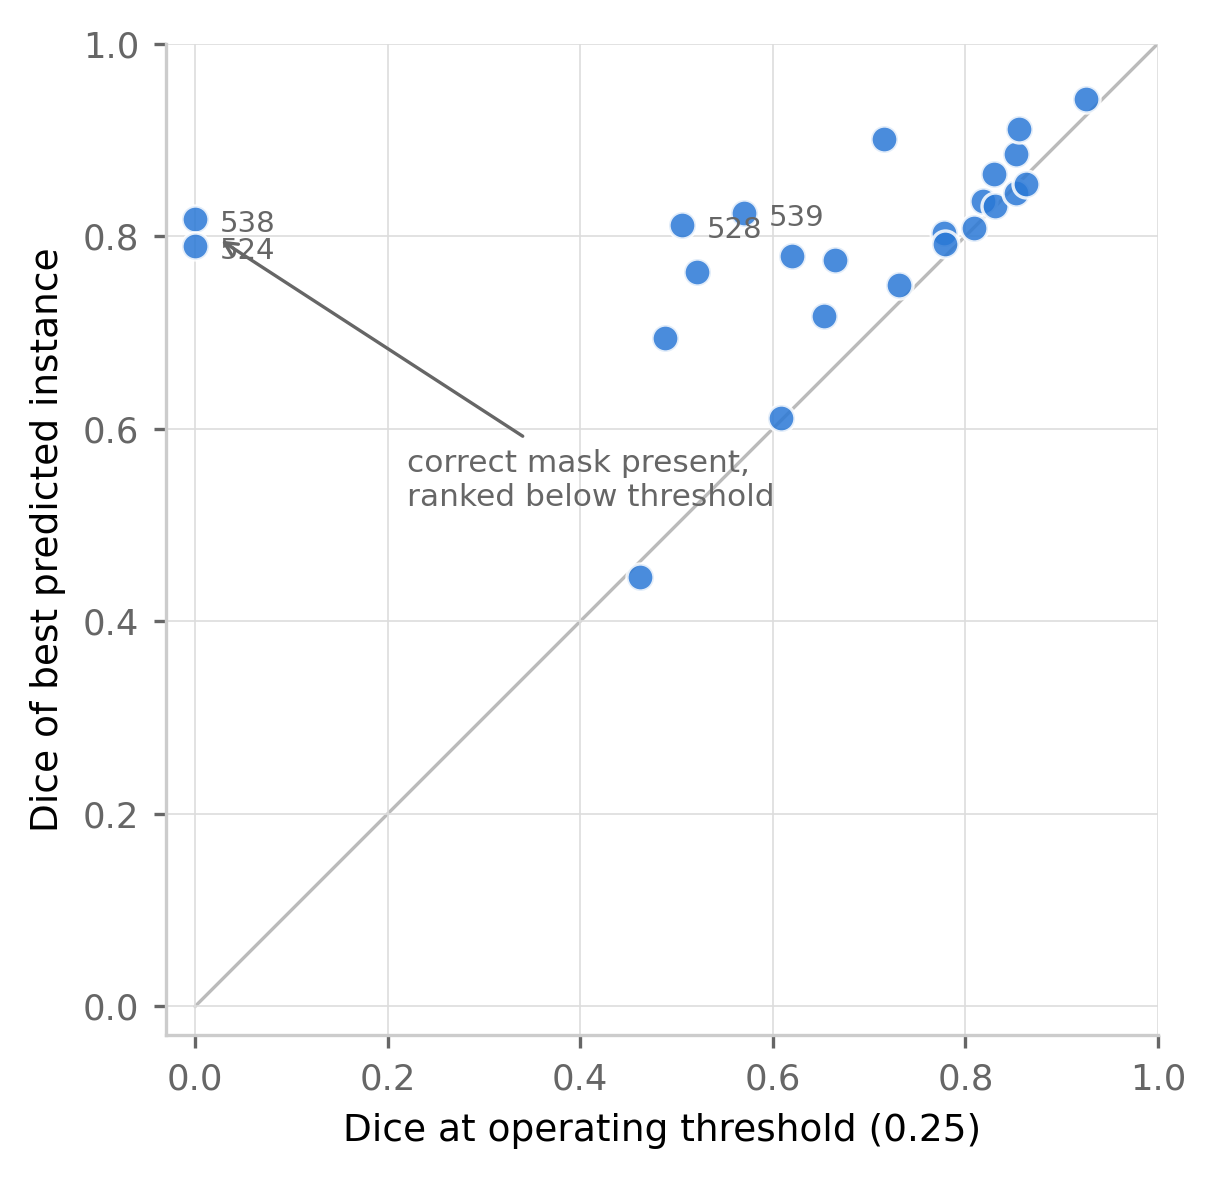
\includegraphics[width=0.58\textwidth]{figures/dice_oracle_scatter.png}
\caption[Achieved against attainable overlap]{For each of the 24 plaque-positive test images, the
Dice coefficient obtained at the operating threshold against that of the best predicted instance
irrespective of its confidence. Points on the diagonal are limited by segmentation quality; points
above it carry a correct mask that the confidence ranking discards.}
\label{fig:dice-oracle}
\end{figure}

The same pattern holds for the individual models (Table~\ref{tab:oracle}), where the gap
between the achieved and the attainable Dice is between 0.18 and 0.21.

\begin{table}[H]
\centering
\caption[Confidence-ranking analysis]{Confidence ranking against segmentation quality on the 24
plaque-positive test images. ``Dice'' is the overlap achieved by the instances the model actually
reports at its operating threshold. ``Dice (best instance)'' is the overlap of the best-matching
predicted instance irrespective of the score it carries, and therefore the ceiling that a perfect
ranking would reach; ``Gap'' is the difference between the two. ``Failures'' gives the number of
plaque-positive images in which no instance reaches the threshold, followed by the number that
would still fail if the best-matching instance were always selected -- so $4 \rightarrow 0$ means
that all four apparent misses are already segmented correctly and only the score prevents them
from being reported. ``Median confidence'' is the score carried by that best-matching instance,
taken across the 24 images.}
\label{tab:oracle}
\begin{tabular}{lrrrrr}
\hline
Model & Dice & Dice (best instance) & Gap & Failures & Median confidence \\
\hline
seg\_v1 (\texttt{cls}~=~0.3) & 0.583 & 0.769 & 0.185 & $4 \rightarrow 0$ & 0.060 \\
seg\_v2 (\texttt{cls}~=~0.3) & 0.547 & 0.754 & 0.207 & $5 \rightarrow 0$ & 0.091 \\
seg\_v3 (\texttt{cls}~=~1.0) & 0.501 & 0.680 & 0.179 & $8 \rightarrow 2$ & 0.602 \\
\hline
\end{tabular}
\end{table}

The classification loss weight controls this directly. Raising it from 0.3 to 1.0 lifts the median
confidence of the correct instance from 0.060 to 0.602, a factor of ten, confirming that the
underweighting described in Section~\ref{subsec:model-training} is the mechanism. It does so at a
cost: the attainable Dice falls from 0.769 to 0.680, and two plaque-positive images no longer
contain a correct mask at all, where seg\_v1 and seg\_v2 leave none. Optimisation pressure moves
from geometry to classification, and the masks pay for it.

The intermediate setting was therefore tested. At \texttt{cls}~=~0.5, seg\_v4 achieves the best
validation performance of all four models (Table~\ref{tab:seg-val}), including the highest mask
precision at 0.766, yet performs worst on the held-out test set. The optimum is bracketed between
0.3 and 1.0 on validation data, but the test set is too small to confirm where it lies.

\subsection{Post-hoc Re-scoring}
\label{subsec:results-rescoring}

Learned re-scoring improved the ranking of individual instances substantially and the image-level
decision not at all. The re-scorer raised the area under the curve for discriminating correct from
incorrect instances from 0.681 to 0.823 on the test set, with grouped cross-validation on the
validation split confirming the improvement (0.705 to 0.796). Applied end to end at matched
quantiles, however, Youden's~$J$ fell from 0.667 to 0.583: sensitivity rose to 100\,\%, recovering
both previously missed images, while specificity fell to 58.3\,\%.

The two objectives differ. The features available to the re-scorer describe what a plaque looks
like, which identifies genuine instances well; but in a plaque-free image the model still proposes
plaque-shaped instances, and the re-scorer promotes those equally. The original confidence,
however poorly calibrated, encodes the absence of a plaque better than any appearance-based
feature. The limiting factor for image-level performance is therefore objectness rather than
instance ranking, and it cannot be repaired after training.

\section{Effect of the Duplicate Images}
\label{sec:results-duplicates}

Four plaque-positive test images are byte-identical to images in the development partition of
the published split (Section~\ref{subsec:duplicates}) and were therefore seen during training.
The partition was used as distributed; the overlap is a property of the dataset rather than of
the split applied here. Excluding the four images leaves
20 plaque-positive and 24 plaque-negative images and lowers the figures of the best configuration
as follows.

\begin{table}[H]
\centering
\caption[Performance with and without the duplicated images]{seg\_v1\,+\,seg\_v2 at the operating
point selected on validation, computed on the full test partition and with the four duplicated
images removed.}
\label{tab:dedup}
\begin{tabular}{lrrrrr}
\hline
& $n_{\text{pos}}$ & Sens. & Spec. & $J$ & Dice \\
\hline
Full test partition & 24 & 0.917 & 0.750 & 0.667 & 0.655 \\
Duplicates excluded & 20 & 0.900 & 0.750 & 0.650 & 0.615 \\
\hline
\end{tabular}
\end{table}

\begin{figure}[H]
\centering
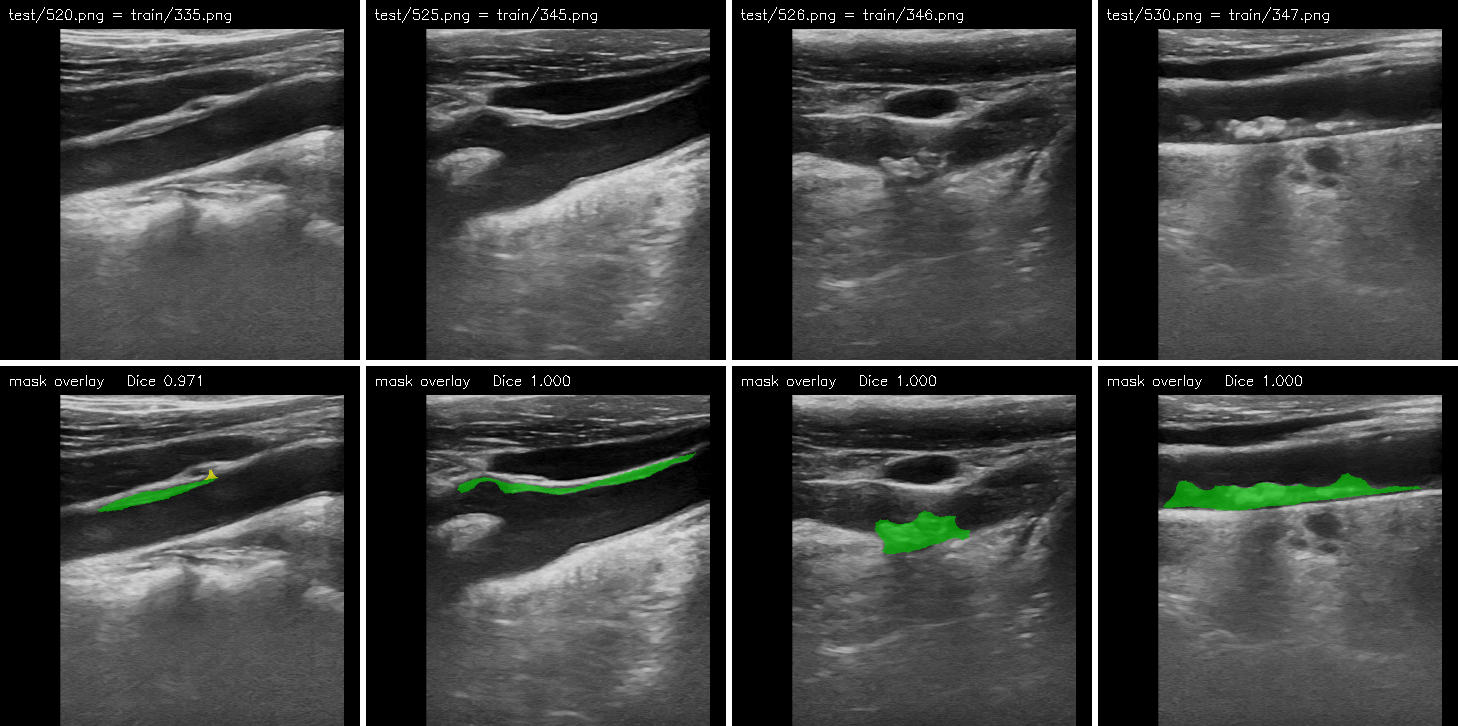
\includegraphics[width=\textwidth]{figures/duplicate_pairs.png}
\caption[Images duplicated across the published split]{The four images appearing in both
partitions of the published split. Top row: the shared image. Bottom row: the two annotations
overlaid -- green where they agree, yellow where only the test-partition mask covers a pixel, red
where only the development-partition mask does. Three pairs carry byte-identical masks. The
first, \texttt{520.png}, was annotated twice independently; the two masks agree at a Dice
coefficient of 0.971, the difference being confined to the distal tip of the lesion.}
\label{fig:duplicate-pairs}
\end{figure}

The four pairs are shown in Figure~\ref{fig:duplicate-pairs}.

The four affected images are among those the model handles best, with Dice coefficients between
0.82 and 0.92, which is consistent with their having been seen in training. The effect on the
aggregate is nonetheless small: Youden's $J$ falls by 0.017 and the mean Dice by 0.040, against a
margin over the base model of 0.192 on the deduplicated set. The deduplicated figures are the
ones this thesis relies on; both are reported so that the comparison with other work using the
published split remains possible.

\chapter{Discussion}
\label{ch:discussion}

\section{Why the Proteomic Analysis Found No Signal}
\label{sec:discussion-phase1a}

Neither the univariate screen nor any of the classifiers recovered an association between the
model-derived plaque phenotype and the plasma proteome. Two explanations are available, they
operate at different levels, and the design of this study cannot separate them.

\subsection{A Biological Explanation}

The first explanation is that established subclinical carotid plaque simply does not produce a
detectable systemic protein signature. Atherosclerosis develops over decades, and the lesions
imaged here are, by the nature of a population imaging cohort, clinically silent. There is no
acute event to detect: no rupture, no thrombus, no inflammatory flare of the kind that would
plausibly register in circulation. What is present instead is a slow, focal accumulation in a
vessel wall, small in absolute terms against the volume of plasma into which anything it releases
would be diluted. A process may be consequential without being measurable, and subclinical plaque
is a plausible instance of that: large in its eventual clinical implications, small in its
contemporaneous biochemical footprint.

The strongest support for this reading comes from within the analysis itself. Age produced a
visible gradient in the leading principal components of the same protein matrix and remained
significantly associated after correction for multiple testing, while plaque status produced
neither. The same cohort, the same measurements and the same procedure detect one and not the
other. The proteome, on this evidence, reflects systemic physiological state rather than the
presence of a focal lesion.

One consideration qualifies the dilution argument. Carotid plaque is generally regarded not as an
isolated local finding but as a marker of systemic atherosclerosis, since subclinical disease is
typically present in several vascular territories at once \cite{fernandezfriera2015pesa}; a
participant with carotid plaque is therefore likely to carry coronary and aortic disease as well. The relevant burden is therefore
larger than the imaged lesion, and the argument from lesion volume holds only to the extent that
the carotid finding is a poor index of total atherosclerotic burden. Subclinical atherosclerosis
at the carotid and femoral sites is associated with coronary calcification
\cite{laclaustra2016femoral}, which suggests the carotid finding indexes more than itself.

\subsection{A Complication from the Same Cohort}

A strong form of the biological explanation is difficult to sustain. In the same UK Biobank
cohort, \textcite{omarov2024deep} report a genome-wide association study of carotid plaque whose
downstream analyses implicate lipoprotein(a) and interleukin-6 signalling, both of which have
been pursued as drug targets. Both are measurable in plasma, and both are present in the
Olink panel used here, as are interleukin-6 receptor, apolipoprotein B, PCSK9 and several matrix
metalloproteinases. The proteins that a causal analysis identifies in this cohort were therefore
measured in this analysis, and none of them emerged.

The resolution lies in the direction of inference. Mendelian randomisation identifies causes, not
consequences: lipoprotein(a) and interleukin-6 are upstream determinants that drive plaque
formation over decades, and a cross-sectional proteomic association would recover them only if
their effect on prevalent plaque status were large enough to survive both attenuation and
correction across 2{,}923 tests.

Two clinical results reported while this thesis was being written illustrate the same gap from
the other direction, and they concern precisely these two pathways. ZEUS, a phase III trial of
the interleukin-6 antibody ziltivekimab in more than 6{,}300 patients with atherosclerotic
disease, chronic kidney disease and raised C-reactive protein
\cite{ridker2026zeusdesign}, achieved the expected reduction in interleukin-6 signalling but
reported a hazard ratio of 0.99 (95\,\% CI 0.88--1.11) for major adverse cardiovascular events
\cite{novonordisk2026zeus, yao2026zeuscommentary}. Lp(a)HORIZON, a phase III trial of
pelacarsen in 8{,}323 patients with elevated lipoprotein(a) and established cardiovascular
disease \cite{cho2025horizondesign}, lowered lipoprotein(a) but did not meet its primary
endpoint of reducing cardiovascular events \cite{novartis2026pelacarsen}. Both targets were engaged; neither produced the
anticipated clinical benefit.

Neither result overturns the genetic evidence, and neither should be read as doing so. Both
trials lowered a long-standing exposure late, in patients whose disease was established and who
were already receiving guideline-directed therapy. The trial designs are published, but the
outcome data rest on company announcements: neither trial had reported in full at the time of
writing, and both should be checked against the eventual publications. What they do is separate two claims that the
genetic evidence alone does not distinguish: that a molecule contributes to how disease develops
across a lifetime, and that its concentration at a given moment is informative about the disease
that has developed. The same distinction governs the analysis performed here. A protein may shape
how a lesion forms over decades without its level at a single blood draw carrying information
about whether that lesion is now present. A molecule can be causal and still be a poor
cross-sectional marker, and the two properties are established by different kinds of evidence.

The claim that the present data support is consequently narrower than the one stated above. It is not that carotid atherosclerosis leaves no trace in blood, but
that established subclinical plaque produces no proteomic signature detectable \emph{as a
consequence} of its presence, under the sample size and phenotype quality available here.

There is a further reason to expect a binary label to be the wrong instrument for this
particular question. Interleukin-6 concentration is associated not with the presence of carotid
plaque but with its echogenicity \cite{yamagami2004il6} -- that is, with a continuous property
of the lesion's composition rather than with whether one is there at all. A phenotype that
records only presence discards exactly that information. If the proteins implicated by the causal
analysis relate to what a plaque is made of rather than to whether it exists, then no amount of
statistical power applied to a binary label would recover them, and the appropriate phenotype
would be a quantitative description of the lesion -- which is what a segmentation model, unlike a
detector, is able to produce.

The nominally significant proteins are of limited help in adjudicating this. Several are
biologically plausible in context -- matrix metalloproteinase 12 is a macrophage elastase with an
established role in plaque remodelling, and latent TGF-$\beta$ binding protein 2 and Fas ligand
have connections to matrix turnover and apoptosis respectively. But all nine of the leading hits
have between 1.6\,\% and 5.4\,\% missing values, against a panel median of 15.4\,\%. Better-measured
proteins carry more information and therefore attract smaller $p$-values irrespective of biology,
and median imputation compresses the variance of sparsely measured proteins and further reduces
their detectability. The ranking is thus confounded with measurement completeness, and the
apparent biological coherence of the top of the list should not be read as evidence.

\subsection{A Measurement Explanation}

The second explanation concerns the phenotype rather than the biology. The plaque labels are not
measurements but model outputs, and a binary exposure measured with error biases estimated
associations towards the null when the error is unrelated to the outcome
\cite{bross1954misclassification, copeland1977bias}. For a binary exposure the attenuation is
exact rather than approximate: the risk difference that such an analysis recovers is the true
risk difference multiplied by the sensitivity and specificity of the classifier minus one --
that is, by Youden's $J$, the same quantity used to evaluate the detection models in
Chapter~\ref{ch:results}. The measure that evaluates the model is therefore also the factor by
which it attenuates whatever the downstream analysis is looking for. On its own UK Biobank test
set the base model attains $J = 0.787$, so roughly a fifth of any true association is lost before
the analysis begins, and more than that on data unlike its development cohort. Combined with a Bonferroni threshold of
$1.7 \times 10^{-5}$ and an analysis cohort of 2{,}542 participants, only a comparatively large
effect could have been detected.

The two explanations are not alternatives so much as statements about different links in the same
chain, and both may hold simultaneously. What matters for the interpretation of this thesis is
that its design cannot distinguish them. A null result is compatible with an absent signal and
with a signal destroyed in measurement, and nothing in the analysis performed here separates the
two cases.

Phase 1B was, in retrospect, precisely the experiment that would have separated them. Relating an
independently derived cardiovascular risk estimate to the same proteomic data would have placed
the question on a phenotype not produced by the imaging model: an association there, alongside
its absence for plaque status, would have implicated the phenotype; its absence in both would
have implicated the proteomic data or the size of the cohort. That this comparison could not be
carried out is the reason the question remains open.

\subsection{An Alternative Design}

Independently of which explanation holds, the design tested prevalent plaque against
contemporaneously measured protein levels. If the proteome reflects the rate at which
atherosclerosis is progressing rather than the burden that has accumulated, a cross-sectional
comparison cannot detect it in principle. A design relating protein levels to incident plaque, or
to progression between two imaging visits, addresses a different and arguably more appropriate
question, and UK Biobank is in the process of assembling the data such a design would need: the
repeat imaging project aims to re-scan 60{,}000 participants, of whom roughly 20{,}000 had
attended by the end of 2025 \cite{ukbiobank_repeat_imaging}. Whether that resource supports a
plaque-progression analysis depends on the repeat protocol including carotid ultrasound, which
is a narrower question than whether repeat imaging exists.

\section{External Validation and Domain Shift}
\label{sec:discussion-domain-shift}

The base model loses 6.2 percentage points of sensitivity and 26.7 of specificity when moved from
the cohort it was developed on to Ar-PlaqSegm1. The asymmetry is the informative part. The model
still finds the plaques that are present; what it loses is the ability to recognise their absence.

\subsection{The Loss Is Not a Threshold Artefact}

An obvious objection is that the confidence threshold of \textcite{omarov2024deep} was tuned on
UK Biobank and simply does not transfer. The data answer this. At the threshold selected on the
validation split the base model reaches $J = 0.458$; the best value attainable anywhere on the
test set, with the threshold chosen on the test set itself, is 0.500. Re-tuning recovers 0.042 of
the 0.329 that separates external from in-cohort performance. The remainder is a change in what
the model represents, not in where its decision boundary is placed.

\subsection{Why Specificity Rather Than Sensitivity}

The composition of the external dataset offers a concrete explanation. Ar-PlaqSegm1 enrolled
patients with mild, moderate or severe atherosclerosis and a vascular wall thickness exceeding
1\,mm (Section~\ref{subsec:external-dataset}). Its plaque-free images are therefore not images of
healthy vessels: they are images of thickened, diseased vessels that happen not to contain a
focal plaque. In a population cohort the plaque-free class consists largely of unremarkable
vessels, and a model trained there learns a correspondingly permissive notion of what counts as
normal.

This is consistent with what the fine-tuned models get wrong. Their shared false positives follow
the vessel wall over an extended stretch and are systematically thinner than annotated plaques,
20.7 pixels against 29.9 in median thickness. Thickened wall without focal protrusion is exactly
the appearance that an enriched cohort supplies in quantity and a population cohort does not, and
it is exactly the case in which the distinction between plaque and not-plaque is hardest.

The asymmetry is not peculiar to this application. A lung ultrasound classifier developed at a
single centre and evaluated on multicentre data retained a sensitivity of 0.92 while its
specificity fell to 0.76, and fine-tuning on part of the external data raised specificity to 0.82
without changing sensitivity \cite{wu2024generalizability}. The correspondence with the figures
reported here is close: the base model retains 83.3\,\% sensitivity against 62.5\,\%
specificity, and fine-tuning recovers specificity while sensitivity does not decline. What
transfers across data sources appears to be the appearance of the lesion; what does not is the
threshold separating it from a diseased but lesion-free background, which is a property of the
population a model was trained on rather than of the pathology it was trained to recognise.

\subsection{What the Shift Would Do to a Prevalence Estimate}

The practical consequence for a phenotyping pipeline follows from the operating characteristics
alone. A classifier reports a positive rate of $\text{Se} \cdot p + (1 - \text{Sp})(1 - p)$ for a
true prevalence $p$. At the in-cohort values of 89.5\,\% and 89.2\,\%, a cohort with 45\,\% true
prevalence would be reported at 46.2\,\% -- an error of roughly one percentage point. At the
external values of 83.3\,\% and 62.5\,\%, the same cohort would be reported at 58.1\,\%.

The calculation is an illustration of the mechanism rather than a projection. It assumes that
sensitivity and specificity measured on a clinically enriched sample carry over to a population
sample, which spectrum effects make unlikely -- and the preceding subsection argues that precisely
this assumption fails here. What it does show is that a degradation of this size does not merely
make individual classifications less reliable; it biases any aggregate derived from them in a
predictable direction.

\subsection{The Shift Is Not One Thing}

Country, centre, device generation, operator, case mix and acquisition geometry differ
simultaneously between the two datasets, and a single external dataset cannot separate their
contributions. The heterogeneity documented in Section~\ref{subsec:external-dataset} shows that
the last of these varies appreciably even within Ar-PlaqSegm1, across groups whose median
grey-scale intensity differs by nearly a factor of two. What this thesis establishes is the
magnitude of the aggregate shift between two specific datasets, and that it is large enough to
matter for downstream use. Attributing it to particular causes would require external datasets
that vary one factor at a time, which do not currently exist for this task.

\section{What Limits the Fine-Tuned Models}
\label{sec:discussion-calibration}

Fine-tuning on target-domain data recovers roughly half the specificity lost to the shift, and
pooling two models recovers a little more. Neither addresses what actually constrains the models,
which the error analysis identifies as something other than segmentation quality.

\subsection{The Masks Are Already There}

Selecting, for each plaque-positive test image, the best-matching predicted instance irrespective
of its confidence raises the mean Dice coefficient from 0.655 to 0.794 and leaves no image
without a correct mask. The two images the pooled model appears to miss are both outlined
accurately -- one at a Dice of 0.82 -- and both carry confidence scores three orders of magnitude
below the operating threshold. Whatever limits these models, it is not their ability to delineate
a plaque once they have attended to it.

That this traces to a single training hyperparameter is worth stating plainly, because it is
unglamorous and consequential in equal measure. With one class, the classification branch of the
loss \emph{is} the confidence score, and it was weighted twenty-five times below the terms
governing geometry. Raising the weight moved the median confidence of the correct instance from
0.060 to 0.602. It also lowered the attainable Dice from 0.769 to 0.680 and left two images
without any correct mask, so the setting trades one failure mode for the other rather than
removing either.

\subsection{Ranking Is Not the Binding Constraint}

A natural response is to repair the ordering after training, and the attempt is instructive in
failing. A re-scorer using geometry, position and local echo contrast improved the separation of
correct from incorrect instances substantially, from an area under the curve of 0.681 to 0.823,
and recovered both previously missed images. Image-level performance nonetheless fell, from
$J = 0.667$ to 0.583, because specificity collapsed to 58.3\,\%.

The reason is that the two objectives are different. Features describing what a plaque looks like
identify genuine instances well, but a plaque-free image still elicits plaque-shaped proposals,
and the same features promote those equally. The original confidence score, for all its
miscalibration, encodes something the appearance features do not: whether there is anything there
at all. The binding constraint is objectness, and no reordering of proposals can supply it.

\subsection{What the Shared Errors Suggest}
\label{sec:discussion-shared-errors}

Five of the six false positives are produced by both models. Two networks differing in capacity,
input resolution and training schedule converge on the same mistakes, which points away from the
models and towards the data or the task definition. Under the Mannheim criterion \cite{touboul2012mannheim} a plaque is a
focal protrusion exceeding 50\,\% of the \emph{surrounding} intima-media thickness -- a relative
judgement requiring a comparison between a candidate region and its neighbourhood. A model that
scores each region on its own appearance has no access to that comparison, and thickened
non-focal wall is the case in which the omission shows.

One candidate explanation can be set aside. Annotation variability is not the limiting factor:
one image of the dataset occurs twice and carries two independently produced masks, which agree
at a Dice coefficient of 0.971 -- well above the 0.62 to 0.79 the models achieve
(Section~\ref{sec:results-duplicates}). A single pair is weak evidence, but it points away from label noise as the
ceiling and towards the models themselves.

If this reading is right, the shared error rate is a rough indication of what cannot be removed
by better training under the present label definition, and improvement would have to come from
encoding the criterion rather than from more capacity or more data. The inference is suggestive
rather than established: two models is a thin basis for a claim about irreducible error, and the
alternative explanation -- that both inherited the same bias from a shared COCO initialisation
and a common augmentation scheme -- is not excluded by the evidence here.

\subsection{A Methodological Note}

The re-scoring result generalises beyond this application. An intervention that improved the
ranking metric by 0.14 area under the curve degraded the decision that the ranking exists to
support. Calibration methods are conventionally assessed on calibration metrics; where the model
feeds a downstream decision, that decision is the only evaluation that settles whether the
intervention helped.

\section{Comparison with the Literature}
\label{sec:discussion-literature}

\subsection{How Much Non-Image Data Contributes}

\textcite{stamos2025} addresses a question adjacent to Phase 1A: whether clinical and biochemical
data, including protein biomarkers, add information to B-mode carotid ultrasound. Three fusion
architectures were evaluated on 73 patients stratified into high- and low-risk groups by degree
of stenosis. The result most relevant here is the decomposition. Imaging alone reached an area
under the curve of 84.6\,\%; the tabular data alone, 64.6\,\%; their fusion, 86.1\,\%. A learned
attention mechanism assigned 69.4\,\% of its weight to the imaging arm.

Two observations follow. First, non-image data carrying only modest standalone signal for a
carotid plaque phenotype is not peculiar to the present work: 64.6\,\% there and the 54.1\,\%
obtained from proteomics here are different tasks on different data, but they occupy the same
regime, well below what the image supplies. Second, and more consequentially, properly fused
end-to-end the tabular data added 1.5 percentage points to an imaging-only model. If that is the
scale of the available gain, then improving the imaging arm is the larger lever, which is the
direction this thesis took for unrelated reasons.

\subsection{Two Ways of Being Data-Limited}

The two studies fail in opposite directions, and the contrast is instructive. \textcite{stamos2025}
has clinically adjudicated risk labels and 73 patients: the ground truth is sound and the sample
is too small to support strong conclusions, as an area under the curve of 86.1\,\% on 73 cases
carries a wide interval. The present work has 20{,}014 participants and a phenotype produced by a
model whose own external validation shows substantial error. Neither configuration permits the
analysis both are reaching for. A study combining adjudicated labels with cohort-scale numbers
does not presently exist for carotid plaque, and until it does, results in this area will be
limited either by their labels or by their size.

It is also worth noting that \textcite{stamos2025} is an instance of the pattern
\textcite{omarov2024deep} identify as limiting the field: a cohort selected for carotid disease
rather than drawn from a population. The concern they raise about generalisability applies to it,
and symmetrically, the concern this thesis raises about phenotype quality applies to their own
population-scale results.

\subsection{Why the Obvious Comparison Is Unavailable}

The fine-tuned ensemble reported here attains 91.7\,\% sensitivity and 75.0\,\% specificity;
\textcite{omarov2024deep} report 89.5\,\% and 89.2\,\%. Setting these against one another would be
a mistake. They come from different datasets with different case mixes, acquisition conditions and
annotators, and the second set was obtained on the cohort the model was developed on while the
first was not. The only comparison this thesis licenses is the one made on a single test partition
in Section~\ref{sec:results-phase2}, where the base model and the fine-tuned models are evaluated
on identical images under an identical protocol.

The difficulty is not peculiar to these two studies. Every result cited in this chapter was
obtained on data held by the group that produced it: \textcite{omarov2024deep} on UK Biobank,
\textcite{stamos2025} on a cohort of 73 patients from one centre, and the present work on
Ar-PlaqSegm1. Each is internally coherent and none can be placed on a common scale with the
others. Reporting guidelines address the related but distinct question of whether a model was
validated outside its development cohort \cite{collins2015tripod, mongan2020claim}; they do
not make results from different external cohorts comparable to each other.

What distinguishes the evaluation reported here is that its test data are public.
Ar-PlaqSegm1 is openly available with a published partition \cite{rulloni2025arplaqsegm1}, so
every figure in Chapter~\ref{ch:results} can be recomputed by others and any future model can be
placed directly alongside them. That is a modest form of comparability, and extending it is the
subject of Section~\ref{sec:conclusion-outlook}.

\section{Limitations}
\label{sec:discussion-limitations}

\subsection{Adaptation, Not Formulation}
\label{subsec:limitations-control}

The comparison in Chapter~\ref{ch:results} places fine-tuned segmentation models against a
detection model that was never adapted to Ar-PlaqSegm1. It therefore confounds two things: the
change of formulation from bounding boxes to masks, and the adaptation to the target domain. A
control experiment was run to separate them. A detector was trained on the same images, the same
split and the same schedule as seg\_v2, differing only in its head and in the absence of
copy-paste augmentation, which requires masks and is unavailable to a box model.

The control reaches the same image-level performance as the segmentation models. At the threshold
selected on validation it attains a sensitivity of 79.2\,\% and a specificity of 83.3\,\%
($J = 0.625$) on the full test partition -- identical to seg\_v1, seg\_v2 and seg\_v3, with an
error profile coinciding exactly with that of seg\_v3. Excluding the duplicated images it reaches
$J = 0.583$, inside the range of 0.525 to 0.600 spanned by the four segmentation models. With 20
plaque-positive images one image corresponds to 0.05 in $J$, so every difference among the
fine-tuned models, the detector included, is smaller than a single image.

What this thesis demonstrates is consequently narrower than it might appear. The improvement over
the base model is attributable to adaptation to the target domain, not to the segmentation
formulation; a detector given the same data performs as well. The domain-shift result in
Section~\ref{sec:discussion-domain-shift} is unaffected, as is the calibration analysis, which
concerns the internal behaviour of the segmentation models rather than their advantage over
detection.

One argument for the segmentation formulation survives the control, because the control cannot
address it. A mask model yields lesion area and shape, and with them the Dice coefficients
reported throughout Chapter~\ref{ch:results}; a detector produces none of these. Where the
intended output is a binary phenotype the two formulations are interchangeable on this evidence,
and where it is a quantitative description of the lesion they are not.

A second control, a segmentation model trained without copy-paste augmentation, would have
separated the head from the augmentation within the segmentation formulation. It was started but
could not be completed, so the detector comparison above remains confounded with that
augmentation. Given that the detector matches the segmentation models despite lacking it, the
confound is unlikely to conceal an advantage rather than create one.

\subsection{Duplicate Images and a Contaminated Validation Split}

Two forms of leakage affect the results, one inherited and one introduced here.

The published split places four plaque-positive images in both partitions
(Section~\ref{subsec:duplicates}). Their effect on the reported figures is quantified in
Section~\ref{sec:results-duplicates} and is small, but it is leakage nonetheless, and any
published result computed on this test partition without deduplication carries the same
optimism.

The second is a consequence of how the development partition was divided here. The 493
development images were split into training and validation strata by plaque presence, but not by
image identity, and seven of the 22 duplicate groups internal to the development partition
straddle that division. Roughly one validation image in ten is therefore a copy of a training
image. Because the validation split selected both the best checkpoint and the confidence
threshold, both selections are mildly optimistic. Correcting this requires deduplicating before
splitting and retraining all configurations, which was not possible within the time available;
the appropriate response is to treat the validation figures as selection scores rather than
performance estimates, which is how they are used throughout.

\subsection{The Test Partition Does Not Span the Dataset}

The 48 test images are not a representative sample of Ar-PlaqSegm1. Grouping the images by
acquisition geometry (Section~\ref{subsec:external-dataset}) shows that 93.8\,\% of the test
partition falls into a single group, which makes up 52.1\,\% of the development partition, and
that three groups comprising 196 development images -- 37.7\,\% of the material available for
training -- are absent from the test partition altogether. The groups are visually and
statistically distinct, differing in median intensity by a factor of nearly two.

Every figure reported in Chapter~\ref{ch:results} therefore characterises performance on a narrow
region of the acquisition conditions the dataset contains. The models were trained across all
groups but evaluated on essentially one, and how they behave on the geometries absent from the
test partition is unknown. This qualifies the external validation in a direction that is easy to
overlook: evaluating on data from a different cohort establishes transfer across cohorts, but not
transfer across the acquisition conditions within the new cohort.

The observation also has a wider implication. If a published dataset that explicitly aims at
diversity -- its authors list the inclusion of varied sizes, locations and multiple plaques as a
design goal -- nonetheless distributes that diversity unevenly across its own partitions, then
comparable imbalances should be expected in evaluation sets generally, including the one on which
the base model was originally validated. Reporting the composition of a test partition, and not
only its size, would make such limitations visible.


\subsection{Statistical Resolution}

The held-out test partition contains 24 plaque-positive and 24 plaque-negative images, and after
excluding the duplicated images, 20 and 24. One image therefore corresponds to between 4.2 and
5.0 percentage points of sensitivity. Differences smaller than that are not measurable, and most
of the differences between the fine-tuned models are smaller than that: on the deduplicated set
the four segmentation models and the detection control span $J = 0.525$ to $0.600$, a range of
one and a half images.

Statements in this thesis are worded to respect that limit, and the conclusions that rest on
larger margins -- the gap to the base model, the size of the confidence-ranking effect -- are
unaffected. But any reading of the results that ranks the fine-tuned variants against one
another, or that treats the ensemble's advantage as established, exceeds what 44 images can
support. Cross-validation over the full development set would give a spread rather than a point
estimate, at a cost of a few training runs; it was not within the time available here.

\subsection{Patient-Level Independence}

The published split separates images, and the four duplicated images aside, no image occurs in
both partitions. The dataset record does not state how many patients the 541 image pairs derive
from, and patient-level independence has therefore not been established. If one patient
contributed images to both partitions, the models would have seen that patient's anatomy,
acquisition device and operator during training, and the test figures would be correspondingly
optimistic. The partition is the dataset authors' own rather than a choice made here, but the
limitation applies to the results regardless of who introduced it.

\subsection{Analytical Choices in Phase 1A}

Two decisions in the proteomic analysis would be made differently on repetition. Imputation and
standardisation were fitted on the full analysis cohort rather than within each cross-validation
fold, which leaks information across the folds; because both operations are unsupervised and the
bias runs towards optimistic performance, the null result reported is if anything conservative.
More consequentially, the clinical baseline used age at recruitment where age at the imaging
visit is the variable matched to the phenotype. The interval between the two is several years and
varies between participants, so the covariate is both shifted and noisy relative to the outcome
it is paired with, and the weak performance of the age-and-sex baseline cannot be cleanly
attributed to the phenotype until the analysis is repeated with the correct variable.

\subsection{One External Dataset}

External validation here rests on a single independent dataset. What the results establish is
that the base model transfers imperfectly to Ar-PlaqSegm1, and that fine-tuning on Ar-PlaqSegm1
recovers part of the loss. Whether the same would hold for a third dataset -- and how much of the
observed shift is attributable to country, centre, device, case mix or annotation practice --
cannot be determined from one comparison. A conclusion about external validity in general would
require several external datasets, as set out in Section~\ref{sec:conclusion-outlook}.

Annotation practice is the one component for which a partial estimate is available. The
duplicated image pair carrying two independently produced masks
(Section~\ref{sec:results-duplicates}) shows agreement at a Dice coefficient of 0.971, which
suggests that annotation variability within this dataset is small relative to the model errors
reported. A single pair is a thin basis for that, and no inter-reader agreement statistics are
published with the dataset.

\chapter{Conclusion and Outlook}
\label{ch:conclusion}

\section{Conclusion}
\label{sec:conclusion}

This thesis set out to identify plasma biomarkers of subclinical atherosclerosis and ended by
examining the phenotype such a search depends on. Three findings summarise the work.

\paragraph{The pipeline was reproduced faithfully, and the phenotype it yields carries little
detectable proteomic signal.}
Re-running the detection pipeline of \textcite{omarov2024deep} across the UK Biobank carotid
ultrasound collection produced detections for 179{,}611 images from 20{,}014 participants and a
plaque prevalence of 43.0\,\% at participant level, against the 45\,\% reported by the original
authors. Tested against the Olink proteomics panel in the 2{,}542 participants for whom both were
available, this phenotype showed no association that survived correction for multiple testing:
151 of 2{,}923 proteins reached nominal significance where approximately 146 are expected by
chance, and the best-performing classifier reached a cross-validated ROC-AUC of 0.541, below the
0.551 attained by age and sex alone. Age itself was significantly associated after correction and
produced a visible gradient in the leading principal components, confirming that the analysis
detects association where association exists.

\paragraph{The base model transfers to an external dataset with a substantial loss of
specificity, and fine-tuning recovers part of it.}
On the 48 held-out images of Ar-PlaqSegm1 \cite{rulloni2025arplaqsegm1}, the base model
reached a sensitivity of 83.3\,\% and a specificity of 62.5\,\%, against 89.5\,\% and 89.2\,\%
on its own UK Biobank test set. Sensitivity therefore declined by 6.2 percentage points and
specificity by 26.7. Four segmentation models fine-tuned on the Ar-PlaqSegm1 development set
were individually indistinguishable from one another on the test set, each reaching a Youden's
$J$ of 0.625 against the base model's 0.458 and differing only in how they distributed their
errors. Pooling the predictions of two of them raised $J$ to 0.667 at a sensitivity of 91.7\,\%
and a specificity of 75.0\,\%, recovering roughly half of the specificity lost to the change of
data source. All operating points were selected on the validation split rather than on the test
set; had they been optimised on the test set, the same configuration would have reported 0.792.

\paragraph{The limiting component is confidence ranking, not segmentation.}
Taking the best-matching predicted instance for each plaque-positive test image, irrespective of
its confidence score, raises the mean Dice coefficient from 0.655 to 0.794 and leaves no image
without a correct mask. Both apparent failures of the pooled model disappear: the most severe is
outlined at a Dice of 0.82 while carrying a confidence of 0.0019, against an operating threshold
of 0.25. The models locate plaques they do not report. This behaviour was traced to the weighting
of the training objective, in which the classification term -- the confidence score, for a single
class -- was weighted twenty-five times lower than the terms governing geometry. Raising that
weight lifted the median confidence of the correct instance from 0.060 to 0.602 but degraded mask
quality, placing the optimum between the two settings tested. Attempting to repair the ranking
after training improved the discrimination of individual instances substantially, from an area
under the curve of 0.681 to 0.823, yet lowered image-level performance: the features that
identify a genuine plaque also promote plaque-shaped predictions in plaque-free images. The
binding constraint is therefore objectness rather than instance ranking, and it is not
addressable post hoc.

\section{Outlook}
\label{sec:conclusion-outlook}

\paragraph{Continuing the biomarker search.}
The analyses of Phases 1A and 1B remain open and can be resumed once access to the UK Biobank
Research Analysis Platform is restored, or if an alternative cohort linking carotid imaging to
proteomics becomes available. The objective that motivated the original design is the one still
worth pursuing: a health-record-based proxy for the imaging phenotype, fitted where imaging and
records coexist and then evaluated wherever records exist. It would lift the proteomic analysis
from 2{,}542 participants to the full Olink set, and a null result at that sample size would
carry weight that a null result at 2{,}542 cannot.

Two considerations govern whether such a proxy would work. The first is its own accuracy: the
proxy inherits the error of the imaging phenotype it is fitted against and adds its own, so the
attenuation argument of Section~\ref{sec:domain-shift} applies twice over, and the ceiling on
what it can detect is set by the model examined in the third part of this thesis. The second is
specificity. A proxy built from age, blood pressure, lipids and diagnostic codes predicts plaque
through the risk factors that cause it, and plasma proteins are themselves associated with those
risk factors; an association between proxy and proteome could therefore reflect the risk-factor
profile rather than the lesion. Establishing that the proxy carries information about plaque
beyond its inputs -- for instance by testing whether it improves on those inputs alone within the
2{,}542 participants where the imaging phenotype is available -- is a prerequisite for
interpreting anything found at the larger sample size.

Two smaller changes to the original design are also warranted. The clinical baseline should use
age at the imaging visit rather than age at recruitment, since the plaque phenotype derives from
the former and the interval between the two varies between participants. And the comparison
against an independent risk estimate, which Phase 1B was also to provide, would still help
determine whether the null result originates in the phenotype or in the proteomic data.

\paragraph{Avoiding the discrete phenotype altogether.}
The attenuation argument that motivates this thesis applies to a pipeline that first reduces an
image to a binary label and then correlates that label with molecular data. End-to-end multimodal
fusion, in which image and tabular data enter a single model jointly, never forms the discrete
phenotype and therefore does not incur the associated loss of information. The approach is
established across medical imaging and health-record data more generally
\cite{huang2020fusion}, and \textcite{stamos2025} reports an instance of it for carotid
plaque risk stratification, with imaging contributing the greater part of the signal and tabular
data a smaller complement. Applying it at cohort scale, with the imaging arm initialised from a
model of the kind developed here, is a natural continuation.

\paragraph{Making results comparable across studies.}
Section~\ref{sec:discussion-literature} sets out why the published figures for carotid plaque
detection cannot be compared with one another: each was obtained on data held privately by the
group that produced it. The evaluation reported here differs in that its test partition is
public, so the figures can be recomputed and any later model placed beside them without
renegotiating data access. Generalising that is less a methodological problem than a matter of
convention. Several openly available carotid ultrasound datasets, from different centres, devices
and case mixes, together with the practice of reporting on all of them, would turn the aggregate
domain-shift estimate obtained here into a decomposition by factor: how much of the loss is the
device, how much the population, how much the operator. Evaluating on one external dataset
establishes that transfer is imperfect; evaluating on several would establish why.

\paragraph{Establishing which differences are real.}
The four fine-tuned models could not be separated on 48 test images, in which one image
corresponds to 4.2 percentage points of sensitivity. Conclusions about the classification loss
weight, the choice of architecture or the value of ensembling therefore rest on differences that
the available evaluation set cannot resolve. Cross-validation over the full development set would
provide a mean and a spread instead of a single point estimate, at a cost of roughly five
training runs.

\paragraph{Encoding the diagnostic criterion.}
The false positives that both models share follow the vessel wall over an extended stretch
rather than enclosing a focal protrusion, and are systematically thinner than true plaque
annotations. This is consistent with a model that classifies each candidate region on its own
appearance, whereas the diagnostic criterion is relative: a plaque exceeds 50\,\% of the
\emph{surrounding} intima-media thickness. Supplying that comparison explicitly -- by segmenting
the wall as a second class, or by providing local wall thickness as an additional input -- would
target the dominant failure mode directly, rather than hoping the model infers the criterion from
examples.

\paragraph{Using the discarded frames.}
Main-axis selection reduced 179{,}611 UK Biobank images to 42{,}954, discarding 76\,\% of the
material. Carotid ultrasound acquisitions are cine loops, and the discarded frames carry motion
information that a single-frame model cannot use. Spatiotemporal approaches to plaque
characterisation have been proposed but are computationally demanding; whether they repay that
cost at cohort scale is untested.

\paragraph{Extending the annotated material.}
The one test image that no model segments correctly even under ideal confidence ranking, and the
smallest plaque in the test set, both point to under-represented regions of the training
distribution: plaques in the smallest 6\,\% of the annotated size range are supported by only 28
training instances. Targeted annotation of small and atypical plaques would address this more
efficiently than uniformly enlarging the dataset.

\paragraph{Closing remark.}
This thesis set out to look for molecular markers of a disease and ended by examining how that
disease is measured. The two are not separate undertakings. An association study is bounded by
the quality of the variables it relates, and where one of those variables is produced by a model
rather than observed, the error of that model becomes part of the epidemiology. The proteomic
analysis returned no signal, and nothing established here settles whether that is because no
signal exists or because the phenotype was too coarse to carry one. What the work does establish
is how large the measurement gap becomes outside the cohort the model was built in, which part of
it is the representation and which the threshold, and that in one specific respect the gap is
smaller than it appears: the models outline plaques they decline to report, and the deficit lies
in how the training objective was weighted rather than in what the network can see. Examining the
instrument before trusting what it measures is not a detour from the biological question; it is
the step the answer rests on.

\chapter*{Code Availability}
\addcontentsline{toc}{chapter}{Code Availability}

All code written for this thesis is available at
\todo{Insert the repository URL and state the licence. If the repository is private, say under
what conditions it can be made available, and give the commit hash or release tag corresponding
to the results reported here so that the version is unambiguous.}

\section*{Scripts}

The repository follows the two-block division used in this thesis: \texttt{block1\_cohort}
holds the work carried out on UK Biobank, \texttt{block2\_detection} the work on Ar-PlaqSegm1.
Each block separates scripts from results, and data locations are resolved centrally by
\texttt{common/paths.py} so that the scripts run independently of the working directory. The
pipeline is organised as standalone scripts rather than notebooks, so that each stage can be
re-run without manual intervention.

\begin{description}[leftmargin=2.8cm,style=nextline,nosep,itemsep=3pt]
  \item[\texttt{preprocess\_ukb\_files.py}] Extracts the UK Biobank image archives and writes the
        manifest consumed by the inference script.
  \item[\texttt{run\_plaque\_inference.py}] Applies the base detection model across the manifest
        and writes image-level detections and per-participant plaque counts.
  \item[\texttt{merge\_main\_axis.py}] Aggregates the long-axis selection into per-participant
        image counts.
  \item[\texttt{prepare\_yolo\_seg\_dataset.py}] Converts the Ar-PlaqSegm1 masks into YOLO
        polygon labels and writes the stratified training and validation split.
  \item[\texttt{prepare\_yolo\_det\_dataset.py}] Derives the corresponding bounding-box dataset
        used for the detection control.
  \item[\texttt{finetune\_yolo\_seg.py}] Fine-tunes the segmentation models; the four reported
        configurations differ only in the arguments given on the command line.
  \item[\texttt{finetune\_yolo\_det.py}] Trains the detection and no-copy-paste controls under an
        otherwise identical schedule.
  \item[\texttt{evaluate\_seg\_testset.py}] Evaluates a checkpoint on the held-out test partition
        and writes the confidence sweep and per-image results.
  \item[\texttt{compare\_variants.py}] Evaluates single models and pooled combinations on a
        common image set.
  \item[\texttt{threshold\_on\_val.py}] Implements the threshold protocol: selects the operating
        point on the validation split and reports the resulting test figures alongside the
        test-optimised ones.
  \item[\texttt{rescore\_instances.py}] Fits and evaluates the post-hoc instance re-scorer.
  \item[\texttt{make\_appendix\_gallery.py}] Renders the prediction sheets of
        Section~\ref{sec:appendix-gallery}, re-deriving the operating point from the validation
        split so that the panels and the reported figures cannot diverge.
  \item[\texttt{make\_pr\_curves.py}] Computes the instance-level precision-recall curves of
        Section~\ref{sec:appendix-training} from the validation split.
  \item[\texttt{make\_qualitative\_figure.py},\\\texttt{make\_echogenicity\_figure.py}]
        Render the image figures of Chapters~\ref{ch:introduction} and \ref{ch:results} from the
        dataset and the model checkpoints, so that every panel and every number printed on it is
        recomputed rather than transcribed.
  \item[\texttt{run\_cv.py}] Cross-validation over the full development set; provided for the
        continuation described in Section~\ref{sec:conclusion-outlook} and not used for the
        results reported here.
\end{description}

\section*{Software Environment}

Results were produced with Python 3.12 and the following package versions.

\begin{table}[H]
\centering
\caption[Software versions]{Package versions used for all reported results.}
\label{tab:software}
\begin{tabular}{ll}
\hline
Package & Version \\
\hline
\texttt{ultralytics} \cite{jocher2023ultralytics} & 8.3.248 \\
\texttt{torch} & 2.9.1 \\
\texttt{torchvision} & 0.24.1 \\
\texttt{opencv-python} & 4.12.0.88 \\
\texttt{numpy} & 2.2.6 \\
\texttt{pandas} & 2.3.3 \\
\texttt{scikit-learn} & 1.9.0 \\
\texttt{scipy} & 1.17.1 \\
\texttt{matplotlib} & 3.9.2 \\
\hline
\end{tabular}
\end{table}

Model training used the Metal Performance Shaders backend on Apple silicon; the cohort-scale
inference of Section~\ref{sec:reproduction} ran on cloud instances provided by the UK Biobank
Research Analysis Platform.
The gradient-boosted tree ensemble of Phase 1A used the XGBoost package as provided by the
Research Analysis Platform; the version string is not recoverable now that access has ended, and
is therefore not stated.

\section*{Data}

Ar-PlaqSegm1 is publicly available \cite{rulloni2025arplaqsegm1}. UK Biobank data cannot be
redistributed and are accessible only through the Research Analysis Platform under an approved
application.

\chapter*{Acknowledgements}
\addcontentsline{toc}{chapter}{Acknowledgements}

AI tools such as Claude Code~\cite{anthropic_claude_code} and ChatGPT~\cite{openai_chatgpt} were used to enhance the clarity, grammar, and phrasing of self-written text. The schematic plaque development figure (Fig. 1.1) was created with ChatGPT’s image generation capabilities, All figures showing ultrasound images were generated from the data by the scripts listed in the Code Availability chapter.

This thesis would not have been possible without the support of so many wonderful and inspiring people. I’m really thankful to everyone who guided me along the way and shared this journey with me.

First, I would like to thank Korbinian Träuble for his mentorship, his enthusiasm for sharing the latest developments in \ac{AI} in medicine and \acp{LLM}, as well as giving me the opportunity, to work in a groundbreaking field with an enormous influence on healthcare with the initial access to the \ac{UKB}. On top of that, a huge thank you for making global work during this project possible, while at the same time contributing directly to saving lives and advancing next-generation health services.
Also, a huge \textit{cheers} to Dr. Matthias Heinig for all the exciting projects and the Helmholtz research group I had the chance to be part of. I’m so glad that our paths kept crossing, each time bringing new and inspiring opportunities to collaborate.
A special thanks goes to Dr. Peter Kastner and his entire group at Roche Diagnostics for making this thesis possible and for giving me the opportunity to become involved in their research at the Roche campus in Penzberg.

I am deeply thankful to my mum, my dad, my sister, and the rest of my family for supporting and encouraging me throughout my studies and throughout my life. Thank you for even giving me the opportunity to start over in a study programme that, at the beginning, none of us really knew much about. Taking that chance ultimately led me to a field I have come to love and, perhaps most importantly, to meeting friends for life.

\chapter*{Abbreviations}
\addcontentsline{toc}{chapter}{Abbreviations}

\begin{acronym}[SCORE2-OP]
\acro{AI}{Artificial Intelligence}
\acro{ANOVA}{Analysis of Variance}
\acro{AUC}{Area Under the Curve}
\acro{BH}{Benjamini-Hochberg}
\acro{CLAIM}{Checklist for Artificial Intelligence in Medical Imaging}
\acro{cIMT}{Carotid Intima-Media Thickness}
\acro{COCO}{Common Objects in Context}
\acro{CVD}{Cardiovascular Disease}
\acro{DFL}{Distribution Focal Loss}
\acro{DICOM}{Digital Imaging and Communications in Medicine}
\acro{FDR}{False Discovery Rate}
\acro{GPU}{Graphics Processing Unit}
\acro{GWAS}{Genome-Wide Association Study}
\acro{HDL}{High-Density Lipoprotein}
\acro{HESIN}{Hospital Episode Statistics Inpatient records}
\acro{IMT}{Intima-Media Thickness}
\acro{IoU}{Intersection over Union}
\acro{LLM}{Large Language Model}
\acro{mAP}{Mean Average Precision}
\acro{MPS}{Metal Performance Shaders}
\acro{MR}{Mendelian Randomisation}
\acro{PCA}{Principal Component Analysis}
\acro{PPV}{Positive Predictive Value}
\acro{RAP}{Research Analysis Platform}
\acro{ROC}{Receiver Operating Characteristic}
\acro{SCORE2}{Systematic Coronary Risk Evaluation 2}
\acro{SCORE2-OP}{Systematic Coronary Risk Evaluation 2 -- Older Persons}
\acro{SD}{Standard Deviation}
\acro{TRIPOD}{Transparent Reporting of a multivariable prediction model for
  Individual Prognosis Or Diagnosis}
\acro{UKB}{UK Biobank}
\acro{YOLO}{You Only Look Once}
\acro{YOLACT}{You Only Look At CoefficienTs}
\end{acronym}

% Note: the acronym package is loaded with [printonlyused], so entries that
% never appear in the text are omitted from the printed list automatically.
% Use \ac{...} on first mention in the body text if you want the expansion to
% be inserted for you; plain text mentions do not register as uses.


\printbibliography[title = {References}, heading=bibintoc]

\chapter{Appendix}
\label{ch:appendix}

\section{Predictions on the Complete Test Partition}
\label{sec:appendix-gallery}

Figures~\ref{fig:gallery1} to \ref{fig:gallery3} show the output of the pooled v1+v2 model on
every one of the 48 held-out test images, so that the aggregate figures of
Chapter~\ref{ch:results} can be checked against the individual cases they summarise. The
confidence threshold is the value selected on the validation split, $t^{*} = 0.25$; nothing is
tuned to the images shown. Plaque-positive images are given first, ordered by file number, the
plaque-free images after them.

Two patterns are visible across the sheets. Where the model agrees with the annotation it tends to
agree closely, and the residual disagreement is usually one of extent rather than location: the
predicted region follows the same lesion but stops short of the annotated boundary or continues
past it. Where it fails on a plaque-free image, the predicted region is a thin ribbon running
along the vessel wall rather than a focal protrusion --- the failure mode discussed in
Section~\ref{sec:discussion-shared-errors}.

\begin{figure}[H]
\centering
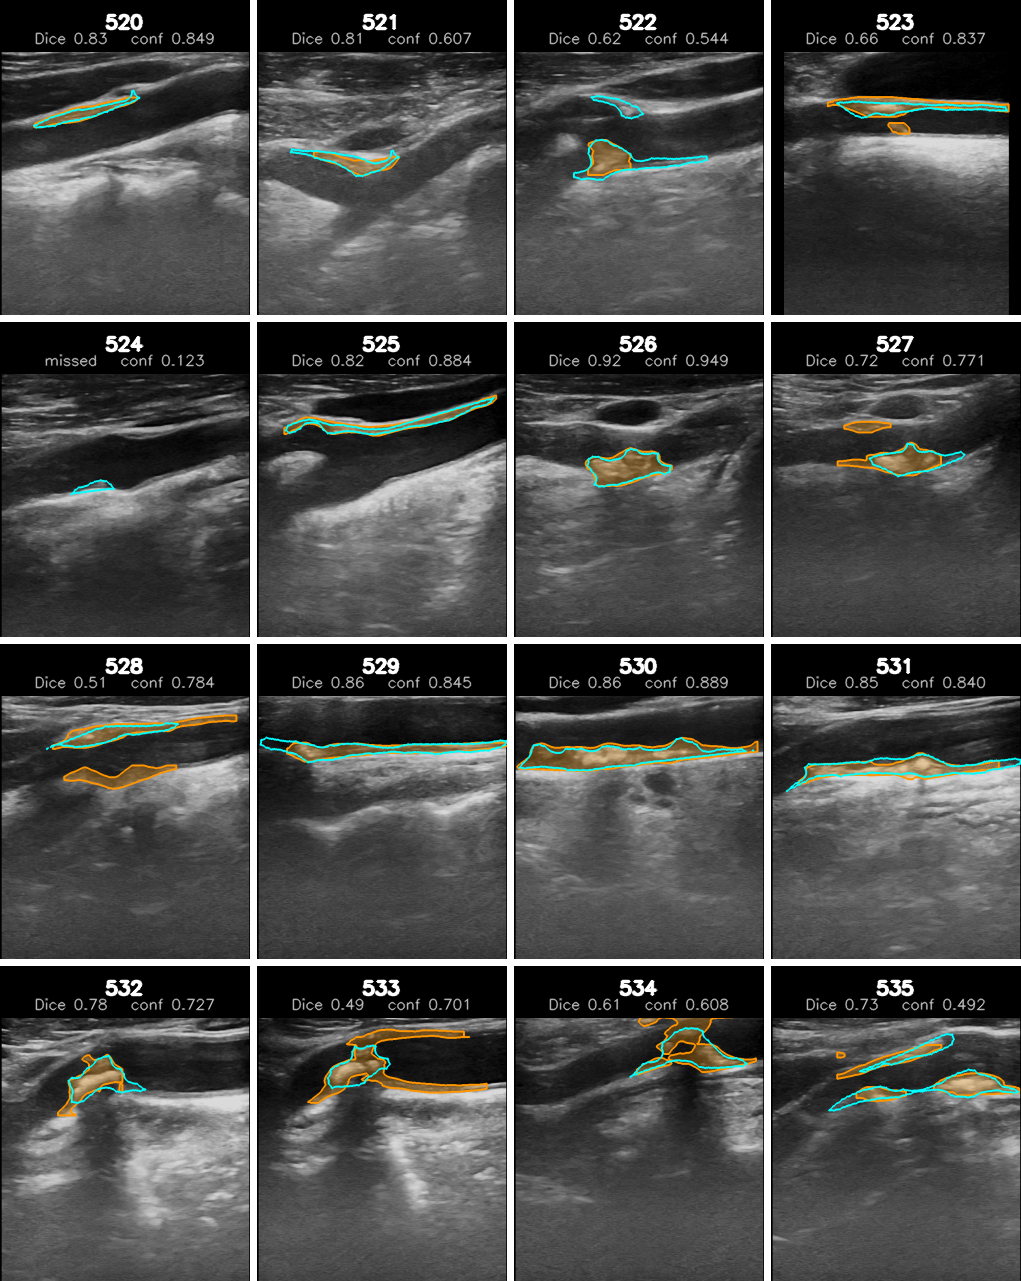
\includegraphics[width=\textwidth]{figures/appendix_gallery_1.png}
\caption[Test-set predictions, part 1]{Pooled v1+v2 predictions on test images 520--535, all
plaque-positive. The annotation is outlined in cyan, the prediction in orange with a light fill.
Each panel gives the Dice coefficient of the prediction against the annotation and the confidence
of the highest-scoring instance; ``missed'' marks an image in which no instance reached
$t^{*} = 0.25$.}
\label{fig:gallery1}
\end{figure}

\begin{figure}[H]
\centering
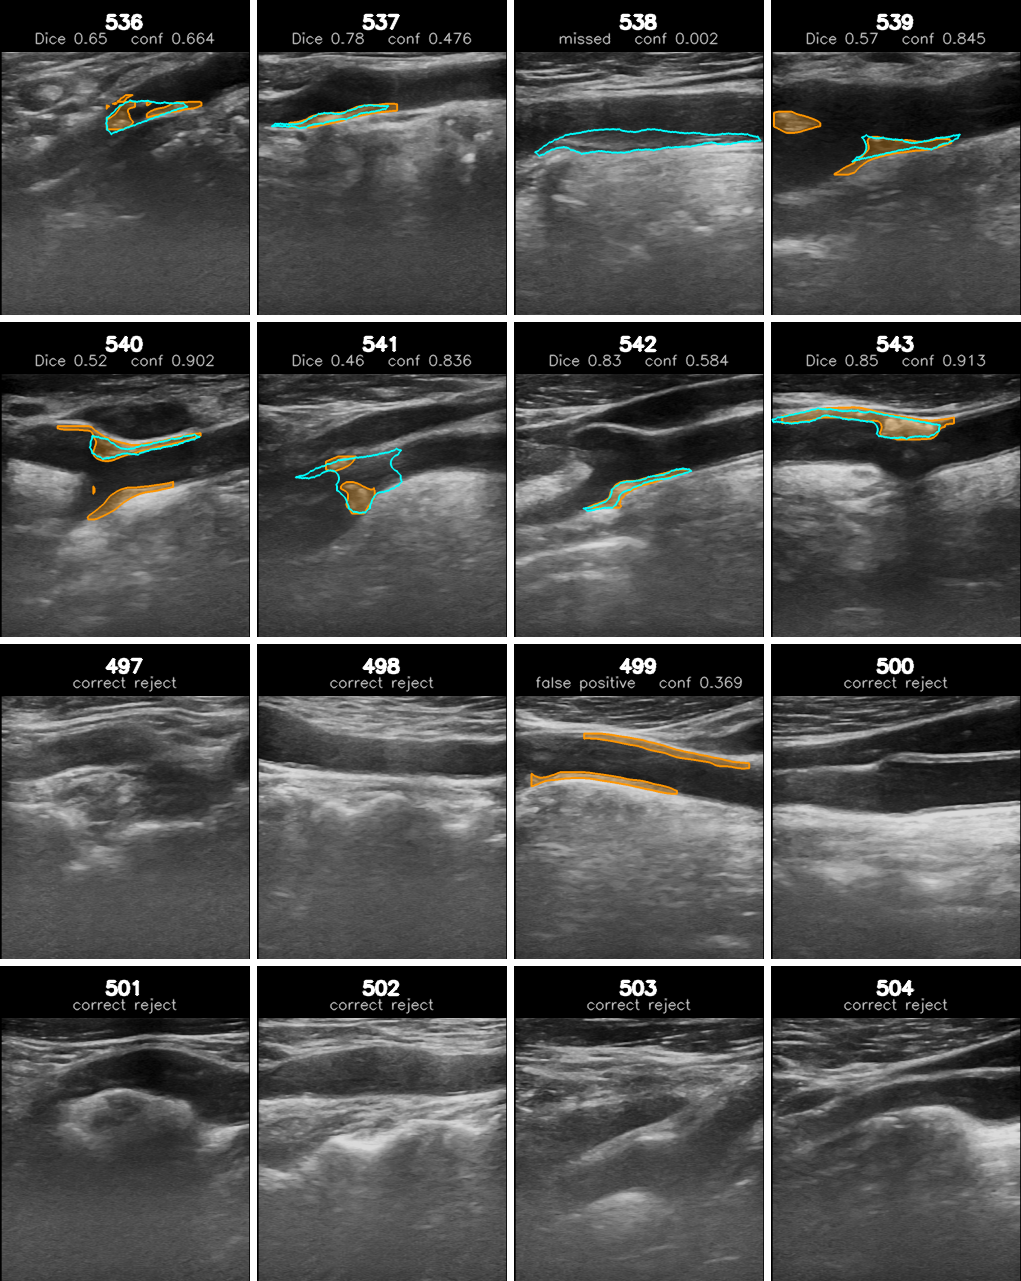
\includegraphics[width=\textwidth]{figures/appendix_gallery_2.png}
\caption[Test-set predictions, part 2]{Continuation of Figure~\ref{fig:gallery1}: the remaining
plaque-positive test images, followed by the first plaque-free ones. Colours and annotations as
in Figure~\ref{fig:gallery1}.}
\label{fig:gallery2}
\end{figure}

\begin{figure}[H]
\centering
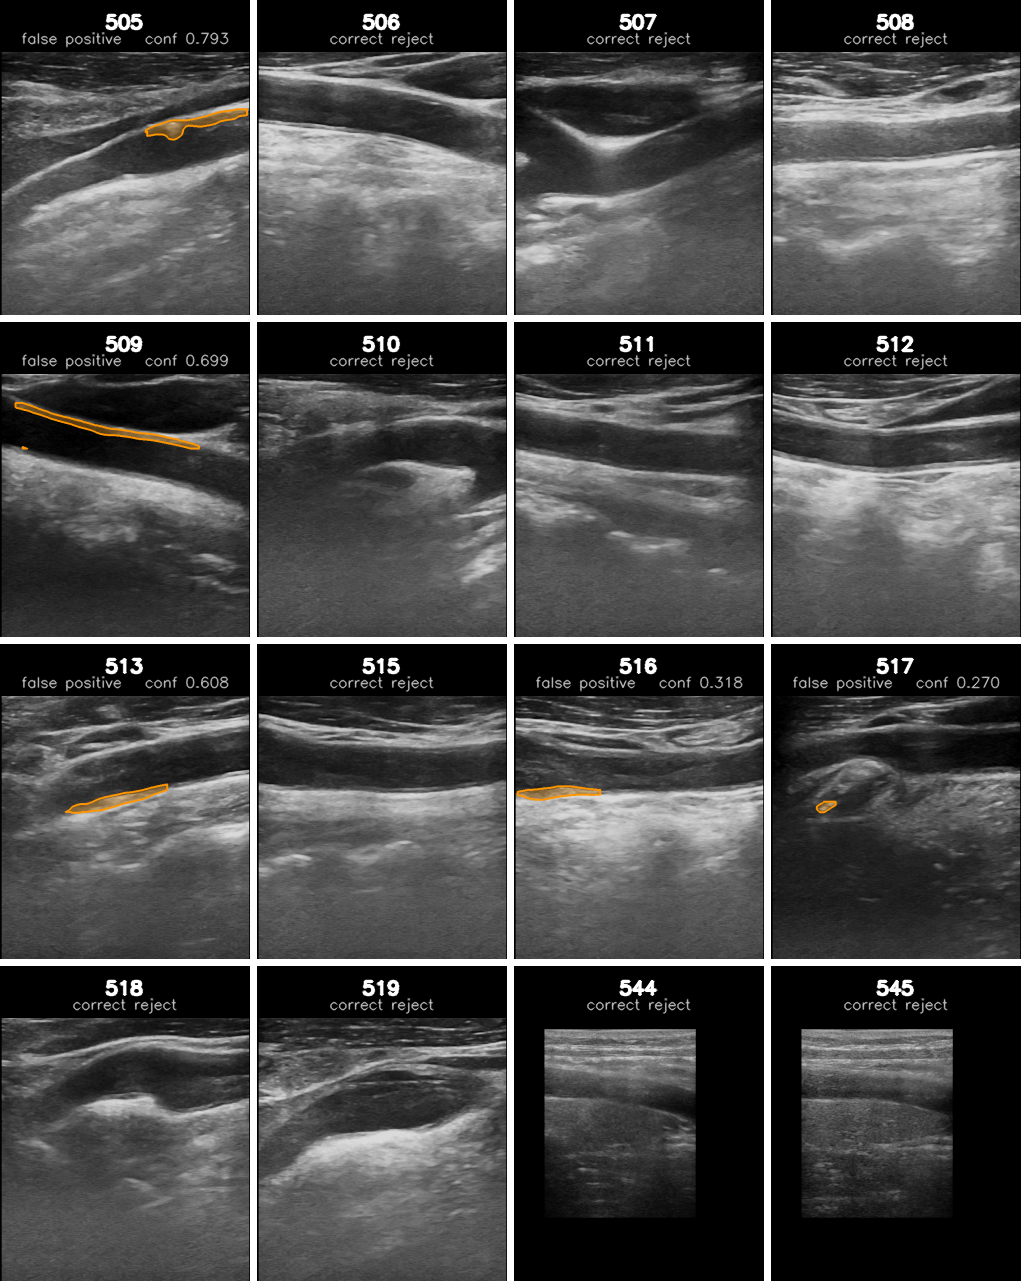
\includegraphics[width=\textwidth]{figures/appendix_gallery_3.png}
\caption[Test-set predictions, part 3]{The plaque-free test images. ``Correct reject'' marks an
image in which no instance reached the threshold; where one did, the panel is labelled as a false
positive and the predicted region is shown. The two images in the lower right were acquired with
the second device and differ visibly in field of view and gain.}
\label{fig:gallery3}
\end{figure}

\section{Per-Image Test Results}
\label{sec:appendix-per-image}

\begin{longtable}{lcccccccc}
\caption[Per-image test results]{Per-image results on the 48 held-out test images at the
operating points selected on the validation split. ``GT'' marks whether a plaque is annotated;
$\dagger$ marks the four images that also occur in the development partition. Check marks give
the image-level decision of seg\_v1, seg\_v2 and their union. ``Dice'' is the overlap achieved by
the union at its threshold, ``best'' the overlap of the best predicted instance irrespective of
its score, and ``conf'' the confidence that instance carries. Plaque-positive images are listed first, in the same order as Figures~\ref{fig:gallery1} to \ref{fig:gallery3}.}
\label{tab:per-image}\\
\hline
Image & GT & v1 & v2 & v1+v2 & Dice & best & conf \\
\hline
\endfirsthead
\hline
Image & GT & v1 & v2 & v1+v2 & Dice & best & conf \\
\hline
\endhead
\hline
\endfoot
520 & +$\dagger$ & \checkmark & \checkmark & \checkmark & 0.83 & 0.86 & 0.707 \\
521 & + & \checkmark & $\times$ & \checkmark & 0.81 & 0.81 & 0.607 \\
522 & + & \checkmark & \checkmark & \checkmark & 0.62 & 0.78 & 0.006 \\
523 & + & \checkmark & \checkmark & \checkmark & 0.66 & 0.77 & 0.012 \\
524 & + & $\times$ & $\times$ & $\times$ & 0.00 & 0.79 & 0.013 \\
525 & +$\dagger$ & \checkmark & \checkmark & \checkmark & 0.82 & 0.84 & 0.826 \\
526 & +$\dagger$ & \checkmark & \checkmark & \checkmark & 0.92 & 0.94 & 0.938 \\
527 & + & \checkmark & \checkmark & \checkmark & 0.72 & 0.90 & 0.003 \\
528 & + & \checkmark & \checkmark & \checkmark & 0.51 & 0.81 & 0.002 \\
529 & + & \checkmark & \checkmark & \checkmark & 0.86 & 0.85 & 0.053 \\
530 & +$\dagger$ & \checkmark & \checkmark & \checkmark & 0.86 & 0.91 & 0.889 \\
531 & + & \checkmark & \checkmark & \checkmark & 0.85 & 0.85 & 0.610 \\
532 & + & \checkmark & \checkmark & \checkmark & 0.78 & 0.80 & 0.012 \\
533 & + & \checkmark & \checkmark & \checkmark & 0.49 & 0.69 & 0.006 \\
534 & + & \checkmark & \checkmark & \checkmark & 0.61 & 0.61 & 0.529 \\
535 & + & \checkmark & \checkmark & \checkmark & 0.73 & 0.75 & 0.004 \\
536 & + & \checkmark & \checkmark & \checkmark & 0.65 & 0.72 & 0.001 \\
537 & + & \checkmark & $\times$ & \checkmark & 0.78 & 0.79 & 0.016 \\
538 & + & $\times$ & $\times$ & $\times$ & 0.00 & 0.82 & 0.002 \\
539 & + & \checkmark & \checkmark & \checkmark & 0.57 & 0.82 & 0.845 \\
540 & + & \checkmark & \checkmark & \checkmark & 0.52 & 0.76 & 0.104 \\
541 & + & \checkmark & \checkmark & \checkmark & 0.46 & 0.45 & 0.005 \\
542 & + & $\times$ & \checkmark & \checkmark & 0.83 & 0.83 & 0.584 \\
543 & + & \checkmark & \checkmark & \checkmark & 0.85 & 0.89 & 0.765 \\
497 & -- & \checkmark & \checkmark & \checkmark & -- & -- & -- \\
498 & -- & \checkmark & \checkmark & \checkmark & -- & -- & -- \\
499 & -- & $\times$ & \checkmark & $\times$ & -- & -- & -- \\
500 & -- & \checkmark & \checkmark & \checkmark & -- & -- & -- \\
501 & -- & \checkmark & \checkmark & \checkmark & -- & -- & -- \\
502 & -- & \checkmark & \checkmark & \checkmark & -- & -- & -- \\
503 & -- & \checkmark & \checkmark & \checkmark & -- & -- & -- \\
504 & -- & \checkmark & \checkmark & \checkmark & -- & -- & -- \\
505 & -- & $\times$ & $\times$ & $\times$ & -- & -- & -- \\
506 & -- & \checkmark & \checkmark & \checkmark & -- & -- & -- \\
507 & -- & \checkmark & \checkmark & \checkmark & -- & -- & -- \\
508 & -- & \checkmark & \checkmark & \checkmark & -- & -- & -- \\
509 & -- & $\times$ & $\times$ & $\times$ & -- & -- & -- \\
510 & -- & \checkmark & \checkmark & \checkmark & -- & -- & -- \\
511 & -- & \checkmark & \checkmark & \checkmark & -- & -- & -- \\
512 & -- & \checkmark & \checkmark & \checkmark & -- & -- & -- \\
513 & -- & $\times$ & $\times$ & $\times$ & -- & -- & -- \\
515 & -- & \checkmark & \checkmark & \checkmark & -- & -- & -- \\
516 & -- & $\times$ & $\times$ & $\times$ & -- & -- & -- \\
517 & -- & $\times$ & $\times$ & $\times$ & -- & -- & -- \\
518 & -- & \checkmark & \checkmark & \checkmark & -- & -- & -- \\
519 & -- & \checkmark & \checkmark & \checkmark & -- & -- & -- \\
544 & -- & \checkmark & \checkmark & \checkmark & -- & -- & -- \\
545 & -- & \checkmark & \checkmark & \checkmark & -- & -- & -- \\
\end{longtable}


\section{Instance-Level Performance of the Fine-Tuned Models}
\label{sec:appendix-training}

Chapter~\ref{ch:results} compares the fine-tuned models at the image level, which is the quantity
the downstream analyses consume. Figure~\ref{fig:appendix-pr} gives the complementary view at the
instance level, where each predicted plaque is matched against the annotation individually.

The four curves lie close together over the whole range, which is the same conclusion the
image-level evaluation reaches by a different route: the configurations differ in how they
distribute their errors rather than in how many they make. Two features are worth noting. None of
the models exceeds a recall of about 0.86 even at the lowest confidence, so a minority of
annotated instances is never produced at all. And precision falls below 0.5 well before that
point, so the instances added at low confidence are predominantly spurious --- which is why the
confidence threshold matters as much as it does, and why the ranking analysis of
Section~\ref{subsec:results-calibration} concerns the ordering rather than the masks.

\begin{figure}[H]
\centering
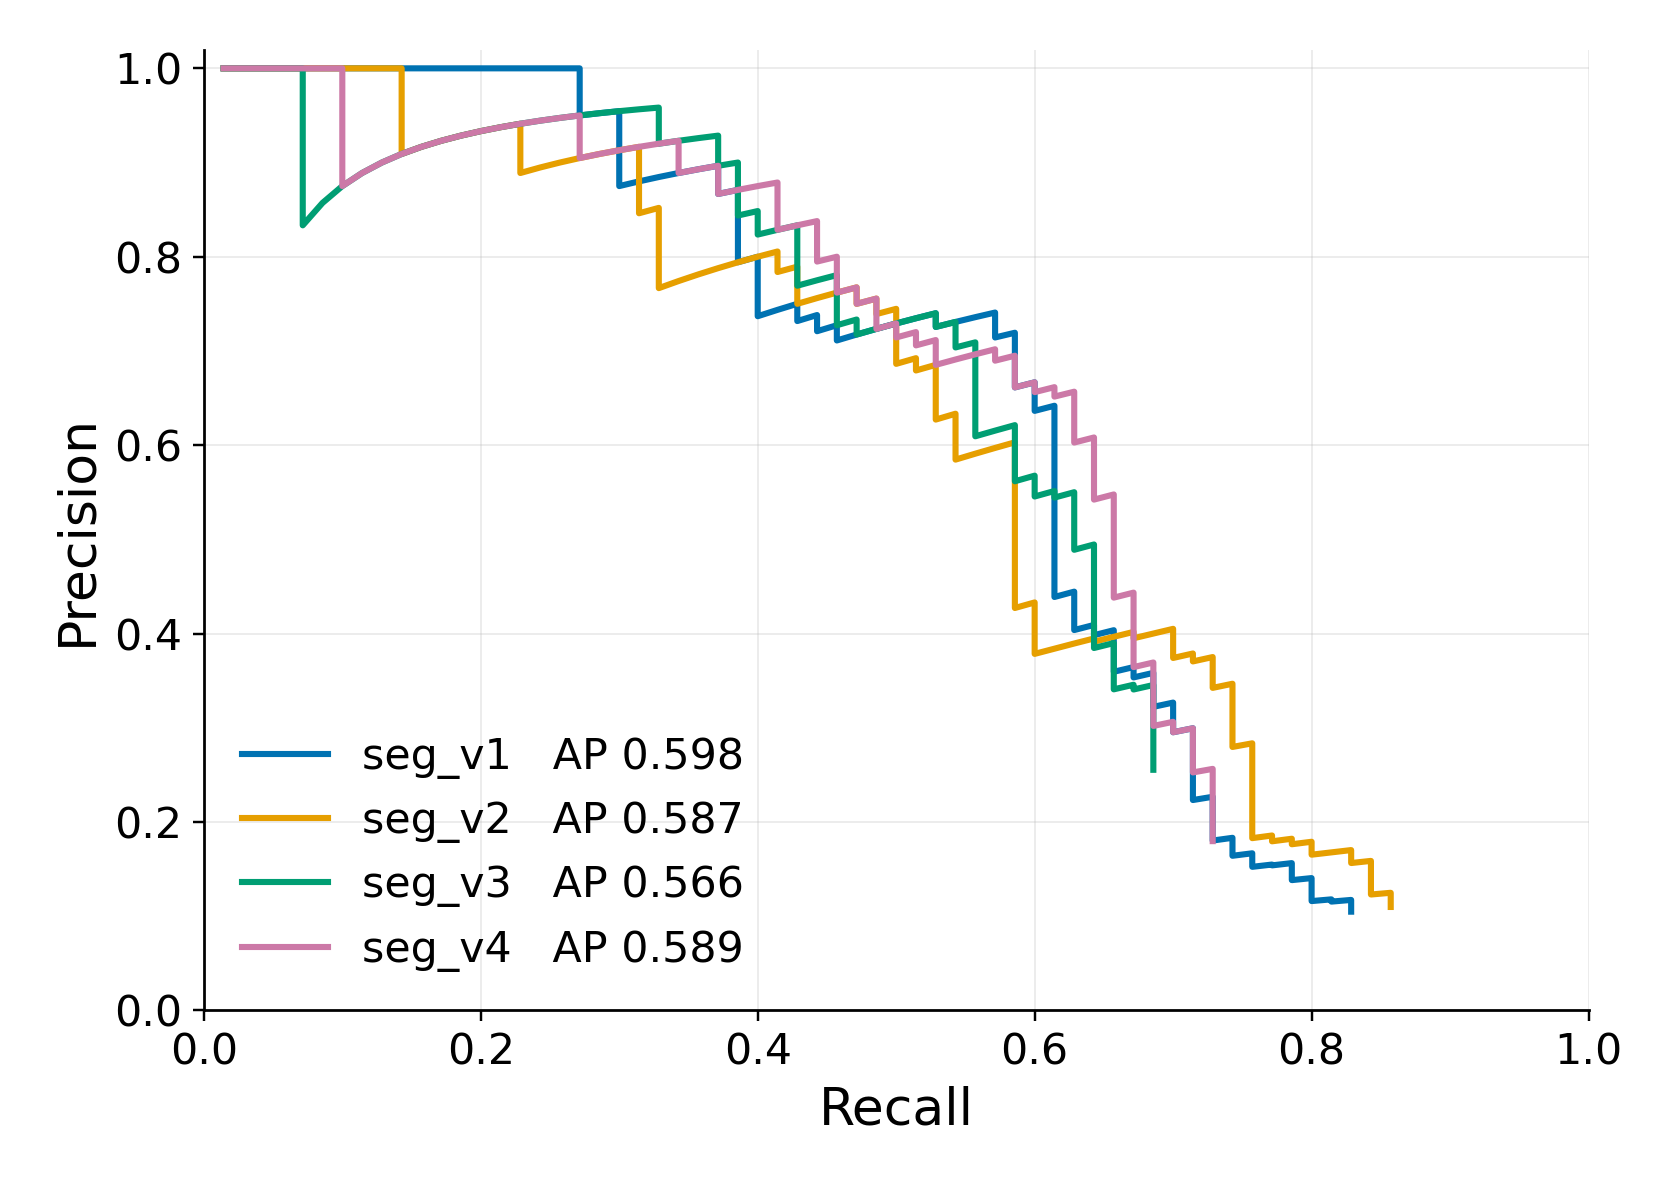
\includegraphics[width=0.86\textwidth]{figures/pr_curves.png}
\caption[Instance-level precision-recall curves]{Mask precision-recall curves of the four
fine-tuned configurations on the validation split. A predicted instance counts as a true positive
if its mask intersection over union with an as yet unmatched annotated instance reaches 0.5;
instances are matched in descending order of confidence, so each annotation is claimed at most
once. The legend gives the average precision, the area under the interpolated curve. The
evaluation covers 70 annotated instances across the 73 validation images.}
\label{fig:appendix-pr}
\end{figure}






\end{document}
